%\input{tcilatex}

\documentclass[12pt,reqno]{amsart}
%%%%%%%%%%%%%%%%%%%%%%%%%%%%%%%%%%%%%%%%%%%%%%%%%%%%%%%%%%%%%%%%%%%%%%%%%%%%%%%%%%%%%%%%%%%%%%%%%%%%%%%%%%%%%%%%%%%%%%%%%%%%%%%%%%%%%%%%%%%%%%%%%%%%%%%%%%%%%%%%%%%%%%%%%%%%%%%%%%%%%%%%%%%%%%%%%%%%%%%%%%%%%%%%%%%%%%%%%%%%%%%%%%%%%%%%%%%%%%%%%%%%%%%%%%%%
\usepackage{amsfonts}
\usepackage[samelinetheorem,notitle]{maherart}
\usepackage{enumerate}
\usepackage{bm}
\usepackage{bbm}
\usepackage{tikz}
\usepackage{float}
\usepackage{booktabs}
\usepackage{threeparttable}
\usepackage{siunitx}
\usepackage{array}
\usepackage{adjustbox}
\usepackage{amsmath}
\usepackage{amsthm}
\usepackage{xcolor}
\usepackage[normalem]{ulem}
\usepackage{cancel}
\newcommand{\redremoved}[1]{\textcolor{red}{\sout{#1}}}
\newcommand{\redadded}[1]{\textcolor{red}{#1}}
\newcommand{\redremovedmath}[1]{\textcolor{red}{\cancel{#1}}}
\newcommand{\blueadded}[1]{\textcolor{blue}{#1}}
\newcommand{\redcut}[1]{\textcolor{red}{[\textit{Removed:} #1]}}
\usepackage{chngcntr}
\usepackage{textcomp}
\usepackage{esint}
\usepackage{paralist}
\usepackage{graphics}
\usepackage{epsfig}
\usepackage{graphicx}
\usepackage{longtable}
\usepackage{caption}
\usepackage{url}
\usepackage{epstopdf}
\usepackage{multirow}
\usepackage{pdflscape}
\usepackage{natbib}
\makeatletter
\newcommand\fs@boxedtop
  {\fs@boxed
   \def\@fs@mid{\vspace\abovecaptionskip\relax}%
   \let\@fs@iftopcapt\iftrue
  }
\makeatother
\floatstyle{boxedtop}
\floatname{framedbox}{Procedure}
\newfloat{framedbox}{tbp}{lob}

\setcounter{MaxMatrixCols}{10}
%TCIDATA{OutputFilter=Latex.dll}
%TCIDATA{Version=5.50.0.2960}
%TCIDATA{<META NAME="SaveForMode" CONTENT="1">}
%TCIDATA{BibliographyScheme=BibTeX}
%TCIDATA{LastRevised=Tuesday, July 16, 2019 08:42:14}
%TCIDATA{<META NAME="GraphicsSave" CONTENT="32">}

\hypersetup{
    pdftitle =
        {The Wisdom of the Crowd and Higher-Order Beliefs},
    pdfauthor =
        {Yi-Chun Chen, Manuel Mueller-Frank and Mallesh M Pai},
    pdfsubject=
        {The Wisdom of the Crowd and Higher-Order Beliefs}
}
\newcommand{\mb}{\bm}
\newcommand{\mc}{\mathcal}
\newcommand{\mr}{\mathrm}
\newcommand{\mbb}{\mathbb}
\newcommand{\msc}{\mathscr}
\newcommand{\scf}{social choice function}
\newcommand{\tci}{truthful continuous implementation}
\renewcommand{\Re}{\mathbb{R}}
\newcommand{\bt}{t}
\newcommand{\bti}{t_i}
\newcommand{\btmi}{t_{-i}}
\newcommand{\tti}{\tilde{t}_i}
\newcommand{\uxi}{\underline{\xi}}
\newcommand{\bxi}{\overline{\xi}}
%\input{tcilatex}
\newcommand{\tsiw}{\tilde{s}_{i,\omega}}
\newcommand{\ts}{\tilde{s}}
\newcommand{\tmu}{\tilde{\mu}}
\newcommand{\yc}[1]{{\textcolor{red}{#1}}}

\usepackage{thmtools}
\usepackage{thm-restate}

\newcommand{\mmp}[1]{\textcolor{orange}{[MP: #1]}}

\definecolor{goodblue}{HTML}{0969B3}
\begin{document}
\raggedbottom
\emergencystretch=2em
\title{The Wisdom of the Crowd and Higher-Order Beliefs}
\author[Chen]{Yi-Chun Chen$^\text{A}$}
\address{$^{\text{\MakeLowercase{a}}}$Department of Economics and Risk
Management Institute, National University of Singapore\\
\href{mailto:ecsycc@nus.edu.sg}{ecsycc@nus.edu.sg}}
\author[Mueller-Frank]{Manuel Mueller-Frank$^\text{B}$}
\address{$^\text{\MakeLowercase{b}}$IESE Business School, University of
Navarra\\
\href{mailto:mmuellerfrank@iese.edu}{mmuellerfrank@iese.edu}}
\author[Pai]{Mallesh M. Pai$^\text{C}$}
\address{$^\text{\MakeLowercase{c}}$Department of Economics, Rice University%
\\
\href{mailto:mallesh.pai@rice.edu}{mallesh.pai@rice.edu}}
\address{\today}
\thanks{We are especially grateful to Paul Huang Enze for his exceptional research assistance on this paper, including helping with executing the experimental work. We also thank Samuel Ho, Mingzi Niu, Hang Shao, and Xinhan Zhang for excellent research assistance. We thank Itai Arieli, Rahul Deb, Ben Golub, Tai-Wei Hu, Yanwei Jia, Scott Kominers, Ran Smorodinsky, Tom Wilkening; and seminar/conference audiences at a16z Crypto Research, Caltech, Games 2020, IIM Ahmedabad, Bonn, IDEAL Institute at Northwestern, and the Summer Game Theory Workshop 2025 for helpful comments and discussions.  Chen gratefully acknowledges the financial support from the Singapore Ministry of Education Academic Research Fund Tier 1. Mueller-Frank gratefully
acknowledges the financial support of the Spanish Ministry of Science,
Innovation and Universities (Ref. ECO2015-63711-P: MINECO/FEDER, UE) and the
Department of Economy and Knowledge of the Generalitat de Catalunya (Ref.
2017 SGR 1244). Pai gratefully acknowledges support from the NSF
(CCF-1763349). The paper source files, the experimental data, and the full open-source replication package are publicly available at \url{https://github.com/malleshpai/robust-aggregation}. }

\begin{abstract}
We propose a new simple procedure called \emph{Population-Mean-Based Aggregation} (PMBA) that enables a principal to ``aggregate'' information about an unknown state of the world from agents without understanding the information structure among them. PMBA only requires agents to communicate their beliefs about the state, and some agents to communicate their expectations of the population average belief. In a large population, for any finite number of possible states, and under weak assumptions on the information structure,  we show that PMBA infers the true state almost surely. A variant of PMBA continues to do so even if agents' beliefs about population averages are misspecified, as long as aggregate misspecification is not too large. We show how PMBA can be reinterpreted as a linear regression procedure, and how it can be used to aggregate information from a finite number of agents, allowing us to reuse existing results on inference in linear models.  We run an experiment with four states. PMBA has lower mean absolute error than simple averaging of beliefs and plurality voting, and does about as well as the Surprisingly Popular procedure when the four states are grouped into two.

\bigskip

\textsc{Keywords:} aggregating beliefs, higher-order beliefs, wisdom of the crowd. \\
\noindent \textsc{JEL Classification:} D82, 
% Asymmetric and Private Information - Mechanism Design
D83.\end{abstract}

% Title page for title and abstract only.
\maketitle


\section{Introduction}
A long-held belief, starting from at least Aristotle, is that of the ``wisdom of the crowd''. This refers to the idea that even though some event may be uncertain, and the information each individual has may be noisy, the ``aggregate'' of individual beliefs is accurate. Such aggregation obviously has large social and private value, especially when it concerns important social or economic events.
As a consequence, there has been substantial effort toward both improving existing institutions (e.g., polling), and designing and implementing new methods (e.g., prediction markets).%
\footnote{There is also a large and influential body of literature that studies the possibility of such aggregation within our current institutions, e.g., voting (see e.g.,~\cite{austen1996information},~\cite{feddersen1997voting}), markets (e.g.,~\cite{grossman1980impossibility}) and social networks (see e.g.,~\cite{golub2010naive},~\cite{acemoglu2011bayesian}).}
At a theoretical level, then, it is important to understand the limits of such an exercise: without specific assumptions on the nature of the information agents have, how can we aggregate it, and how much can we learn from it? In short, how wise is the crowd, and how can we tap into its wisdom?

To fix ideas, imagine a population of interest and an event whose realization is uncertain. Individual agents each see a signal that is informative of the realization. Agents also understand the informational environment, i.e., what this signal implies for their own beliefs and the implied distribution of other agents' beliefs. Even assuming away the difficulties (both logistical and strategic) of eliciting the relevant information from the population, the question we address in this paper is: Does there exist a general procedure to aggregate individuals' information without knowledge of the information structure among them? Our procedure is aimed at applications in which beliefs are evidence about the truth/ realization, e.g. a regulator deciding whether to approve a new drug cares about whether it works, and expert opinion matters to her insofar as it is informative about this.

One important insight from the existing literature is that even if the state is binary, and agents' signals are i.i.d.\ conditional on the state, knowing the first-order beliefs of even an infinite set of agents is generally insufficient to learn the state.\footnote{See~\cite{prelec2017solution} and~\cite{arieli2017crowd}.} In particular, even in these idealized conditions, most agents may be wrong, i.e., most agents may place a posterior probability of larger than 50\% on the incorrect state of the world. The main takeaway from~\cite{arieli2017crowd} is that without further strong assumptions about the signal structure, the principal cannot learn the state of the world from solely agents' first-order beliefs, even with an infinite number of agents in the population. In econometric terms, there is an identification problem.

We answer our question in the affirmative by proposing a novel, simple procedure we name \emph{Population-Mean-Based Aggregation} (herein PMBA). Our procedure uses agents' beliefs about the uncertain event as well as some agents' expectations of the population mean belief. Under weak conditions on the information structure generating the agents' signals, this procedure \emph{fully aggregates} the information among agents in a large population. In other words, using information from agents, solely about agents' own beliefs, and their expectations of the average belief in the population (the \emph{population average belief}), but with no other knowledge of the underlying information structure, we can fully learn the underlying state. Importantly, we show that our procedure is \emph{robust}: it allows for aggregation of beliefs even when beliefs are misspecified at both the individual and aggregate levels. That is, we start from a ``correctly specified'' model where agents share a common prior and form beliefs and higher-order beliefs based on their private information, and show that our PMBA procedure correctly aggregates agents' information without knowledge of the underlying common prior.  In Appendix~\ref{sec:robust}, we show that a variant of this procedure continues to correctly aggregate even if agents' beliefs about the population averages are misspecified (individually, perhaps substantially), as long as aggregate misspecification is not too large (in a sense we make precise there). We show how this procedure can be reinterpreted as a linear regression procedure, and how it can be used to aggregate information from a finite number of agents (\cite{libgober2025wisdom} also recovers an information structure by regression, from a richer set of reports, see Section~\ref{sec:linear}). The machinery of linear regression then allows us to show various forms of robustness of our procedure. In short, our procedure is a viable candidate to be used in practice.  

The idea of eliciting and using higher-order beliefs is not new. In our context, we note the elegant ``Surprisingly Popular'' (herein, SP) procedure developed by~\cite{prelec2017solution} (henceforth PSM), who pioneered the use of second-order beliefs for the purpose of information aggregation (however, their procedure aggregates information only for binary states, and they focus on a narrow set of information structures---as PSM themselves note, it can fail with more than two states, see Appendix~\ref{app:counterex} for an example). Roughly, SP asks each agent for her belief and for her forecast of others' beliefs, and picks the answer that turns out to be more popular than predicted (i.e. whose average belief exceeds its average forecast). Another close comparison is to the Surprisingly Confident (SC) procedure of~\cite{doi:10.1287/mnsc.2020.3919}, who also leverage the linearity of the correspondence between beliefs and higher-order beliefs, and its implication for the ordering of average beliefs and average second-order beliefs in each state (see also Theorem~1.4 of~\cite{prelec2017solution} and related approaches by~~\cite{prelec2022general}, described in Section~\ref{sec:rellit}). A key differentiator is that SP/SC are both only guaranteed to work under binary states, i.e., two possible states of the world, and require stronger assumptions more generally, as we discuss below.

In line with this literature, it is important to note that we are solely using agents’ beliefs and  their expectations of the realized population average belief. Such information has been robustly elicited in laboratory and real-world settings, and therefore, our procedure is amenable to implementation.  Indeed, we elicit precisely these reports in an experiment, see Section~\ref{sec:experiment}. By contrast, theoretically feasible procedures that ask agents for more detailed information such as state-contingent beliefs (for example, the agent's expectation of the average belief in the population \emph{conditional} on the true state of the world) may not be reliable or even feasible in practice.  To be clear, our procedure relies on eliciting reports from many agents. It does, however, avoid asking agents to report state-contingent quantities (such as forecasts conditional on a hypothetical state), which laboratory subjects find difficult (see e.g., \cite{charness2009winnerscurse, esponda2014hypothetical, ngangoue2021learning}).
Similarly, we may not be able to elicit the underlying prior; we take seriously the idea that the prior/ex-ante stage is an ``as-if'' assumption.\footnote{See for example the discussion on page 926 in~\cite{gul1998comment}.}

\subsection{Summary of Model and Results}
Our baseline environment (Section~\ref{sec:pmba}) features finitely many states and many agents whose signals are drawn from an information structure that is \emph{unknown to the principal} but understood by the agents. The contributions of the paper can be summarized in three complementary steps:
\begin{enumerate}
    \item \textbf{Large-population benchmark.} Theorem~\ref{thm:pmba} shows that, under weak regularity conditions, the principal can recover the true state by combining the population mean of first-order beliefs with higher-order reports from at least as many agents as there are states.  Using higher-order reports in this way resolves the indeterminacy that defeats procedures based on first-order beliefs alone (even with two states), and takes the use of higher-order reports in SP/ SC beyond binary states---an issue emphasised by~\cite{prelec2017solution}.
    \item  \textbf{Finite samples and robustness.} Section~\ref{sec:linear} reinterprets the inversion step as a linear regression. This gives finite-sample guarantees for recovering the state (Proposition~\ref{prop:linear:finite}), and a bound on how much systematic bias in second-order reports the procedure can tolerate (Section~\ref{sec:bias}). Section~\ref{sec:experiment} uses an IV version to deal with noise in reported beliefs, at the cost of an exclusion restriction that we cannot test. Appendix~\ref{sec:robust} returns to the Bayesian model: an approximate version of PMBA, which pools second-order reports across groups of agents, recovers the state for generic information structures (Theorem~\ref{theorem:GenericAggregation}), and when agents' beliefs about population averages are misspecified (Theorem~\ref{thm:misspecifiedknowledge}).
    \item \textbf{Empirical performance.}  Section~\ref{sec:experiment} reports a new experiment in which subjects forecast NFT price ranges. PMBA has lower mean absolute error than the two mean-belief rules and plurality voting. When the four ranges are grouped into two, it does about as well as SP (12 against 10 correct out of 20 items). That a procedure built for many states can match SP on the grouped binary problem is, we think, encouraging. Of course, with 20 items the experiment is small, and these differences are not precisely estimated.
\end{enumerate}

The core intuition is simple. Suppose the principal elicits each agent's first-order belief about the unknown state. By the law of large numbers, the sample mean converges to the expected population belief in the true state. Without knowing the mapping from states to those expectations, the principal cannot yet identify the state. Let $L$ denote the number of states. By additionally querying $L$ agents whose beliefs are linearly independent for their forecast of the population mean, the law of iterated expectations yields a system of $L$ linear equations whose unique solution is precisely that unknown mapping. The rest of the paper develops the conditions under which this logic survives realistic complications and documents its performance. Section~\ref{sec:rellit} discusses the related literature and the limitations of our approach, and concludes. The appendices contain the proofs, the robustness results for approximate PMBA (Appendix~\ref{sec:robust}), finite populations (Appendix~\ref{sec:finite}), an example of SP with three states (Appendix~\ref{app:counterex}), two extensions: eliciting guesses instead of beliefs, and incentives for truthful reporting (Appendix~\ref{sec:extensions}), and the details of the experiment (Appendix~\ref{app:experiment}).



\section{Population-Mean-Based Aggregation }\label{sec:pmba}
In this section, we introduce our core model; we describe our Population-Mean-Based Aggregation procedure (herein PMBA) and prove its validity. 

\subsection{General Model and Notation}
There is a population of agents, $N=\{1,2, \ldots \}$, which may be countably infinite (this section),  or finite (Appendix~\ref{sec:finite}; Section~\ref{sec:linear} works with a finite sample), with $i$ denoting a generic agent. There is a finite set of $L$ states of the world $\Omega = \{\omega_1, \omega_2, \ldots, \omega_L \}$, so $L=|\Omega|$ is the number of states. The space of feasible beliefs over $\Omega$ is the $(L-1)$-dimensional simplex $\Delta^L$ (i.e., the set of probability vectors in $\mathbb{R}^L$); we denote it by $\Delta(\Omega)$ when emphasizing the state space.

Each agent $i$ observes a signal in a set $S$ with the associated sigma field $\mathcal{F}$. To allow for correlation, let us denote the common prior over $\Omega \times S^N$ by $P$. Given that an agent observes some signal $s \in S$, their posterior belief that the state is $\omega$ is given by $P(\omega\mid s)$. We let $P_{i,\omega}^S$ denote the induced marginal distribution of $P$ over signals for agent $i$ in state $\omega$. Let us denote the posterior beliefs of agent $i$ by $\mu_i(s) \in \Delta^L$ and $\tmu_i$ as the associated random variable. In what follows, the actual signal seen by the agent will often be irrelevant since we are concerned with their beliefs. We will, therefore, suppress the dependence on the signal in our notation. We define
\begin{align*}
    &m_i(\omega) = \mathbb{E}[\tmu_i|\omega].
\end{align*}
In words, $m_i(\omega)$ is the expected belief of agent $i$ in state $\omega$. 

Finally, we define $\bar{\mu}(\omega) = \lim_{n \to \infty} \frac1n \sum_{i=1}^nm_i(\omega)$, and assume throughout that this limit exists (for the given ordering of agents).\footnote{Note that without further assumptions, it is possible that this limit might not exist and/or might be different depending on the ordering of agents.  Simple sufficient conditions (e.g., conditional i.i.d.\ signals) rule out these concerns with an infinite population, and they are moot for any arbitrarily large finite population.} That is, $\bar{\mu}(\omega)$ is the limit of the average of agents' conditional expectations $\mathbb{E}[\tilde{\mu}_i\mid\omega]$; in other words, the expected population average belief in state $\omega$.

Given a vector $x \in \Delta(\Omega)$, we will let $x_{\omega}$ refer to the component corresponding to $\omega$; i.e., $\mu_{i,\omega}$ is the belief of agent $i$ that the state is $\omega$, $\tmu_{i,\omega}$ is the random variable of agent $i$'s belief that the state is $\omega$, etc.

To keep notation consistent across sections, we use the following conventions throughout: hats (e.g., $\hat\mu$) denote sample averages, bars (e.g., $\bar\mu(\omega)$) denote state-contingent population limits, tildes denote random objects before conditioning, and bold symbols denote stacked vectors or matrices of these quantities.



\subsection{PMBA Procedure}\label{sec:infinite}
Before we introduce our aggregation procedure, we introduce the following assumption on the information structure.
\begin{assumption}[No Aggregate Uncertainty]\label{ass:1}
    We make the following assumptions on $P$:
    \begin{enumerate}
    \item Imperfectly informed agents: for each agent $i$, we have that $P_{i, \omega}^S$ and $P_{i, \omega'}^S$ are mutually absolutely continuous with respect to each other.
    \item Summably limited correlation: Conditional on the state, the aggregate dependence among agents' signals is summably small. Formally, for any two agents $i$ and $j$ and state $\omega$, define \[ \chi_{ij}(\omega) := \sup_{E,E' \in \mathcal{F}} \left| P\bigl(s_i \in E,\,s_j \in E' \mid \omega\bigr) - P^s_{i,\omega}(E)P^s_{j,\omega}(E') \right|. \] We assume that, for every state $\omega$, \[ \sum_{n=1}^{\infty} \frac{1}{n^3} \sum_{1\leq i<j\leq n} \chi_{ij}(\omega) <\infty. \] \end{enumerate}
    \end{assumption}

This assumption requires some explanation. The first condition is simply to make the problem interesting/non-trivial: after all, if an agent is perfectly informed, then aggregation is trivial. Next, we need an assumption regarding the correlations between agents' signals. Intuitively, assuming conditionally i.i.d.\ signals is likely overly strong and does not capture the idea that agents' information may be correlated. However, we cannot allow for arbitrary correlation---for example, if all agents' information is perfectly correlated, then effectively, there is only one unique opinion in the population, and no further aggregation is possible. Our condition allows for arbitrary pairwise correlation, including strong correlation among particular groups of agents, but restricts the \emph{aggregate} amount of dependence in a growing population. In particular, the second condition limits the growth of the cumulative pairwise dependence among the first $n$ agents. Thus, the condition does not require correlations to be uniformly small, nor does it impose independence, identical distributions, or stationarity. Assumption \ref{ass:1} ensures that the law of large numbers holds, so that the population average belief is a deterministic function of the state, i.e., in the notation of our model, in any state $\omega$ we have that
    \[
    \text{as } n \to \infty,\;\; \frac1n \sum_{i=1}^n \tilde{\mu}_i \to_{a.s.} \bar{\mu}(\omega).
    \]
We emphasize that while this assumption relaxes the conditional i.i.d.\ assumption that is regularly made, it is a non-trivial assumption. Whether it is sensible or not depends on the context. For instance, in a political context, if all agents are drawing their information from the same few noisy news sources, then there will be correlations in beliefs and our assumption would not be well-motivated for such a setting. Conversely, if we are considering subjective but idiosyncratic product reviews, then the assumption is far more natural. More generally, the clause is intended to capture environments with enough conditional independence for a law of large numbers argument; residual systematic bias/noise is then handled by the misspecification analysis in Appendix~\ref{sec:misspecified}.



\begin{framedbox}[htbp]
  \caption{Population-Mean-Based Aggregation}\label{proc:pmba2}
  \begin{minipage}{0.95\textwidth}
\begin{enumerate}
    \item Elicit, from each agent $i \in N$, their belief $\mu_i$. Given $n$ elicited agents, compute the empirical mean
    \begin{align*}
        \hat{\mu} = \frac1n \sum_{i=1}^n \mu_i,
    \end{align*}
    which converges almost surely to $\bar{\mu}(\omega)$ under Assumption~\ref{ass:1}.
    \item Select $L$ agents $I = \{i_1, i_2, \ldots, i_L \}$. Construct the $L\times L$ matrix $\bm{\mu}$ with rows $\mu_{i_1}^T,\mu_{i_2}^T,\ldots,\mu_{i_L}^T$, and require $\bm{\mu}$ to be full rank. Keep this set of agents fixed as $n$ increases.
    \item Let $s_i$ be the signal seen by agent $i$. Elicit from each of these agents their expectation of the average posterior beliefs in the population (where $\tmu_j$ denotes agent $j$'s random posterior-belief vector), i.e., elicit for each $i \in I$:
    \begin{align*}
        \alpha_i = \mathbb{E}\left[\frac1n \sum_{j= 1}^n \tmu_j \bigg| s_i\right],
    \end{align*}
    using the same sample size $n$ as in Step~1.
    Denote $\bm{\alpha}= (\alpha_{i_1}^T, \alpha_{i_2}^T, \ldots, \alpha_{i_L}^T)^T$.
\item In the limit, solve
    \begin{equation}
    \bar{\bm{\mu}} = \bm{\mu}^{-1} \lim_{n\to\infty}\bm{\alpha}\label{eqn:mainstep2}
    \end{equation}
    Note that the right-hand side is obtained from agents' elicited reports as $n$ increases and therefore $\bar{\bm \mu}$ can be recovered in the limit. That is, the PMBA procedure recovers $L$ state-dependent population average distributions. It then identifies the state $\omega$ whose recovered population average distribution coincides with the limit of the empirical average distribution $\hat{\mu}$.
\end{enumerate}   
For finite $n$, the procedure identifies the state whose estimated population average is closest (in Euclidean distance) to $\hat{\mu}$.
In practice the procedure works with large but finite $n$; Assumptions~\ref{ass:1}--\ref{ass:fullrank} imply that the empirical quantities in Steps~1--3 approach their population counterparts as the sample grows.
  \end{minipage}
\end{framedbox}

Our second assumption ensures point identification. It requires that distinct states lead to different vectors of population-average beliefs, so that the limiting sample mean can be matched to a unique state. The requirement is weak but worth stating explicitly because identification can otherwise fail when expected beliefs coincide.

\begin{assumption}\label{ass:simple}
We assume that $P$ is such that for any two states $\omega$ and $\omega'$, $\bar{\mu}(\omega) \neq \bar{\mu}(\omega')$.
\end{assumption}
Note that while Assumption~\ref{ass:simple} is not directly stated in terms of the primitives of our model ($P$), it should be clear that this is a property that can be easily satisfied.%
\footnote{For example, in the case of finite conditionally i.i.d.\ signals, this property is generically satisfied in the belief space, in the sense of full measure.}
\par

Finally, we need to ensure that the system of equations that constitutes our procedure is well-posed. This is the role of Assumption~\ref{ass:fullrank}.
\begin{assumption}\label{ass:fullrank}
We assume that the set of agents' realized first-order belief vectors spans \(\mathbb{R}^L\) almost surely, i.e., the prior $P$ satisfies
\begin{equation*}
    P\left(\operatorname{span}\{\tmu_i:i\in N\}=\mathbb{R}^L\right)=1.
\end{equation*}

\end{assumption}

We should note that this condition is weak in at least two ways. First, in the standard genericity sense: a generically chosen set of feasible posteriors will be full rank (for details, see Lemma~\ref{lemma:Genericity} in Appendix~\ref{sec:APMBA}). Second, and perhaps more interestingly, even in settings where there are fewer signals than states (e.g., agents can run only a unique binary-outcome experiment whose outcome determines their posterior), as long as the agents can acquire enough independent signals (e.g., conduct a sufficient number of independent experiments), the set of feasible posteriors is full rank. We formally state this claim below---the proof essentially repurposes a lemma of \cite{fu2021full}. Under conditionally i.i.d.\ signals and common signal supports, each feasible posterior with positive probability is realized in the population almost surely. Thus, a full-rank set of feasible posteriors implies that the realized belief vectors span $\mathbb{R}^L$ almost surely. In the following claim, we maintain Part (1) of Assumption~\ref{ass:1}.

\begin{restatable}{claim}{clfullrank}\label{cl:fullrank}
Suppose that signals are conditionally i.i.d.\ draws from a finite set $S$, and Assumption~\ref{ass:simple} is satisfied. If each agent gets $L-1$ independent draws from the same state-dependent distribution $P_{\omega }^{S}$, then Assumption~\ref{ass:fullrank} is satisfied with the compound signal space $%
S^{L-1}$.
\end{restatable}

We are now in a position to state our main result for this setting.
\begin{restatable}{theorem}{thmpmba}\label{thm:pmba}
Suppose the common prior $P$ satisfies Assumptions~\ref{ass:1},~\ref{ass:simple}, and~\ref{ass:fullrank}. Then the state identified by the PMBA procedure (Procedure~\ref{proc:pmba2}) coincides with the realized state of nature almost surely.
\end{restatable}

In words, in a large population PMBA recovers the realized state. We should note what drives this. By the law of iterated expectations, an agent's forecast of the population average belief is (in the limit) a weighted average of the state-dependent population averages $\bar\mu(\omega)$, with her own beliefs as the weights. Therefore $L$ such forecasts, from agents whose beliefs are linearly independent, pin down the $\bar\mu(\omega)$'s (Assumption~\ref{ass:fullrank}), and these in turn identify the state (Assumption~\ref{ass:simple}). Assumption~\ref{ass:1} ensures that, given the state, the population average belief converges to the deterministic $\bar\mu(\omega)$ (Lemma~\ref{lemma:beliefsconcentrate}). This is what makes an agent's forecast a weighted average of the $\bar\mu(\omega)$'s, and it also means that the sample average reveals $\bar\mu(\omega)$ in the realized state. Of course, Theorem~\ref{thm:pmba} is a benchmark: it is a large-population result, and it assumes that forecasts are reported without error. Section~\ref{sec:linear} relaxes both by viewing the same linear relation as a regression, with explicit statistical assumptions on the errors. Appendix~\ref{sec:robust} instead stays within the Bayesian model, but allows agents to misperceive the population averages.







\section{Linear Regression Interpretation}\label{sec:linear}

Regression provides a practical way to implement PMBA with a finite sample and errors in agents' second-order reports. Using reports from more than $L$ agents, the principal can estimate the state-dependent population mean beliefs by ordinary least squares and compare them with the observed average belief. Under explicit statistical assumptions, we quantify the estimation error and give sufficient conditions for correct state recovery.





\subsection{From PMBA to Linear Regression}

To understand how PMBA relates to linear regression, let us start with the
data we collect from each agent. Consider a state space $\Omega=\{\omega_1,%
\dots,\omega_L\}$ with $L\ge 2$ states.

Throughout this section, we write $p_i$ for agent $i$'s first-order belief vector (denoted $\mu_i$ in Section~\ref{sec:pmba}). We initially fix the coordinate corresponding to $\omega_1$ and write $\alpha_i$ for the scalar forecast of its population average (whereas $\alpha_i$ is a vector in Procedure~\ref{proc:pmba2}); the true state may be any $\omega_k$. From each agent $i$, we elicit two pieces of information:

\begin{enumerate}
\item \textbf{First-order beliefs}: A probability vector $%
p_i=(p_{i1},\dots,p_{iL})$ where $p_{ik}$ is agent $i$'s belief that state $%
\omega_k$ is true (these sum to 1).

\item \textbf{Second-order beliefs}: A scalar $\alpha_i$
representing agent $i$'s expectation of the population average belief about
state $\omega_1$, i.e., what agent $i$ thinks the average reported
probability assigned to $\omega_1$ will be.
\end{enumerate}

 By the law of iterated expectations, agent $i$'s second-order belief $\alpha_i$ should be
a weighted average of the population means in each state, where the weights
are her own beliefs. Specifically, if $\bar\mu_k$ represents the average
belief about state $\omega_1$ in the population when the true state is $%
\omega_k$, then agent $i$'s forecast should be:

\begin{equation}
\alpha_i \;=\; \sum_{k=1}^{L} p_{ik}\,\bar\mu_k + \varepsilon_i, \qquad
\mathbb{E}[\varepsilon_i\mid X,\omega]=0,  \label{eq:struct_LR_multi}
\end{equation}

where $\varepsilon_i$ captures individual reporting errors, cognitive
limitations, or rounding mistakes.\footnote{As in Procedure~\ref{proc:pmba2}, the population average includes agent $i$'s own belief. This shifts her forecast by $\frac1n\bigl(p_{i1}-\sum_k p_{ik}\bar\mu_k\bigr)$, i.e. a bias of the kind covered in Section~\ref{sec:bias}, with $|b_i|\le 1/n$. Alternatively, one can ask agents to forecast the average belief of the \emph{other} agents, as we do in Section~\ref{sec:experiment}.}

Equation~\eqref{eq:struct_LR_multi} is linear in the agent's own beliefs, so the unknown means $\bar\mu_k$ can be estimated by regressing forecasts on beliefs. \cite{libgober2025wisdom} also uses a regression of this sort. In a common-prior model with conditionally i.i.d.\ signals, he elicits experts' beliefs about the state and about the distribution of beliefs in the population, and recovers the information structure by regression (and the prior, via an eigenvector equation, under an additional irreducibility condition). We only need the state-dependent population means (a smaller object), since our goal is to identify the state. This section adds a finite-sample analysis of the regression (Proposition~\ref{prop:linear:finite} and Section~\ref{sec:bias}), which we then implement in Section~\ref{sec:experiment}.

\begin{remark}

To estimate the entire population mean belief vector in each state, extend this construction by repeating regression~\eqref{eq:OLS_L} (below) for each response coordinate $d\in\{1,\ldots,L\}$. For coordinate $d$, the dependent variable is the agent's forecast of the population average probability assigned to $\omega_d$.
\end{remark}

\subsection{The Regression Setup}

Because $\sum_{k=1}^{L}p_{ik}=1$ for every agent $i$, the constant regressor is a linear combination of the $L$ belief regressors. Including all $L$ coordinates and an intercept therefore makes the regressors linearly dependent. We can either use all $L$
coordinates without an intercept, or omit one coordinate and include an
intercept. Taking $\omega_L$ as the baseline gives:

\begin{equation}
\alpha_i = \beta_0 + \sum_{k=1}^{L-1} \beta_k\,p_{ik} + \varepsilon_i, \quad
\beta_0:=\bar\mu_L,\quad \beta_k:=\bar\mu_k-\bar\mu_L.  \label{eq:OLS_L}
\end{equation}

 In words, $\beta_0$ is the population average belief when the
baseline state $\omega_L$ is true, and $\beta_k$ captures how much higher
(or lower) the population average belief is when state $\omega_k$ is true
compared to the baseline state. This is now a standard linear regression
where we can estimate the unknown parameters $\beta_0, \beta_1, \ldots,
\beta_{L-1}$ using ordinary least squares.

\subsection{Geometric Intuition}

 The regression also has a simple geometric interpretation, which helps explain why PMBA works. Think of each agent's beliefs as a point in a $(L-1)$%
-dimensional simplex (since probabilities sum to 1). The regression equation
$p_i\mapsto\alpha_i$ maps this simplex onto a hyperplane in the space of
second-order beliefs.

 Note that the slope of this hyperplane along each coordinate direction is precisely what we need to know: how much the population
average belief differs between states. Specifically, the slope along the $k$%
-th direction equals $\beta_k = \bar\mu_k - \bar\mu_L$, which is exactly the
difference in population averages between state $\omega_k$ and the baseline
state $\omega_L$. This argument applies to any finite number of states when
the design has full rank.

Figure~\ref{fig:hyperplane} illustrates this for $L=3$ states. The triangle
represents all possible belief vectors, the colored dots show the true
population means in each state, and the arrows point from the empirical mean
toward the state means. They illustrate matching, rather than the regression
slopes. Once we know these slopes, we can reconstruct the full set of
population means and identify the true state.

% ----------------------------------------------------------
% TikZ figure: hyperplane over the belief simplex (L = 3)
% ----------------------------------------------------------
\begin{figure}[H]
\centering
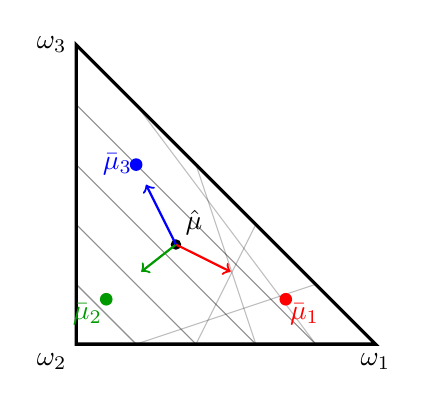
\begin{tikzpicture}[scale=3.8]
      % Simplex vertices
      \coordinate (A) at (0,0);
      \coordinate (B) at (1,0);
      \coordinate (C) at (0,1);
      \draw[very thick] (A)--(B)--(C)--cycle;

      % Vertex labels
      \node[below left]  at (A) {$\omega_2$};
      \node[below]       at (B) {$\omega_1$};
      \node[left]        at (C) {$\omega_3$};

      % Light grid for barycentric intuition
      \foreach \i in {0.2,0.4,0.6,0.8}{
        \draw[thin,opacity=0.25] (\i,0)--(0,\i);
        \draw[thin,opacity=0.25] (1-\i,\i)--(\i,0);
        \draw[thin,opacity=0.25] (0,1-\i)--(1-\i,0);
      }

      % Empirical mean of beliefs
      \fill[black] (0.333,0.333) circle (0.5pt) node[above right] {$\hat\mu$};

      % True state-contingent means
      \fill[red]            (0.70,0.15) circle (0.6pt) node[below right=-2pt] {$\bar\mu_1$};
      \fill[green!60!black] (0.10,0.15) circle (0.6pt) node[below left=-2pt] {$\bar\mu_2$};
      \fill[blue]           (0.20,0.60) circle (0.6pt) node[left=-2pt] {$\bar\mu_3$};

      % Directions from empirical mean to state means
      \draw[->,thick,red]            (0.333,0.333)--(0.516,0.242);
      \draw[->,thick,green!60!black] (0.333,0.333)--(0.217,0.242);
      \draw[->,thick,blue]           (0.333,0.333)--(0.233,0.533);
    \end{tikzpicture}
\caption{Geometric view for $L=3$: the belief simplex (triangle), true
state-dependent population means (coloured dots), the empirical mean $\hat%
\protect\mu$ (black dot), and directions toward the state means (arrows).}
\label{fig:hyperplane}
\end{figure}
% ----------------------------------------------------------

\subsection{Statistical Assumptions}

To make the regression approach rigorous, we need some statistical
assumptions.  Let us stack our data into an $n\times L$ design matrix $X=[%
\mathbf{1}\;p_{i1}\;\dots\;p_{i,L-1}]$ and response vector $%
\alpha=(\alpha_1,\dots,\alpha_n)^{\top}$.

\begin{assumption}[Independent Sub-Gaussian disturbances]\label{ass:linear:subG}
Conditional on the full design matrix $X$ and the realized state, the reporting errors $\varepsilon_i$ are independent across agents, have mean zero, and satisfy
\[
\mathbb E[e^{t\varepsilon_i}\mid X,\omega]\leq e^{\sigma^2t^2/2},\qquad t\in\mathbb R.
\]
For vector responses, this holds coordinate by coordinate with the same bound $\sigma$.
\end{assumption}

These are assumptions on reporting errors. Bounded reports do not imply
mean-zero errors or independence. For example, a shared misunderstanding of
the question can produce correlated errors.

\begin{assumption}[Well-conditioned Gram matrix]\label{ass:linear:LCLN}
The design matrix is well-conditioned with high probability: there exist $\underline\lambda>0$ and $\delta_\lambda\in[0,1)$ such that the event
\[
\mathcal{E}_\lambda:=\bigl\{\lambda_{\min}\!\left(n^{-1}X^{\top}X\right)\ge \underline\lambda\bigr\}
\]
has probability at least $1-\delta_\lambda$, where $\lambda_{\min}(A)$ denotes the smallest eigenvalue of a symmetric matrix $A$.
\end{assumption}

This assumption requires that agents have sufficiently diverse beliefs. If
all agents had identical beliefs, we could not distinguish between different
states because everyone would report the same thing. More generally, if
agents' belief vectors are too similar (nearly collinear), the regression
becomes unstable and we cannot reliably estimate the coefficients.

Different information sources may help, but do not guarantee this condition. Note that with a finite sample, the smallest eigenvalue can be close to zero with positive probability (e.g. when beliefs are conditionally i.i.d.), so we do not require the bound to hold almost surely. Under conditionally i.i.d.\ sampling, if the conditional second-moment matrix of a design row is positive definite in every state, then for a fixed $\underline\lambda$ below the smallest of these eigenvalues, $\delta_\lambda$ tends to zero as $n$ grows.
The constant $\underline\lambda$ measures how ``spread out'' the agents'
beliefs are---larger values mean more diverse beliefs and better estimation.

\begin{remark}[Minimal-information inversion]\label{rem:minimal}
\begingroup
Procedure~\ref{proc:pmba2} inverts a single $L\times L$ matrix built
from $L$ individual reports. For each response coordinate, this inversion is algebraically equivalent to
OLS with exactly $L$ observations and a nonsingular $L\times L$ regressor matrix.
With $L$ coefficients, there are no residual degrees of freedom for estimating standard errors.
\par\endgroup
\end{remark}

\subsection{Finite-Sample Performance}

With these assumptions in place, we can derive concrete performance
guarantees. Using the standard OLS estimator $\widehat{\beta}%
=(X^{\top}X)^{-1}X^{\top}\alpha$ (if $X^{\top}X$ is singular, which can happen only outside $\mathcal{E}_\lambda$, we set the coefficient estimates to zero, and the tie rule below still defines the selected state), we get:

\begin{lemma}[Non-asymptotic error bound]\label{lem:linear:finite}
Under Assumptions~\ref{ass:linear:subG} and~\ref{ass:linear:LCLN}, for any  failure probability $\delta\in(0,1)$, the estimation error is bounded by:
\begin{equation}
  \Pr\Bigl(\|\widehat{\beta}-\beta\|_2 \le
          \frac{\sqrt{L}\sigma}{\underline\lambda}\sqrt{\tfrac{2\log(2L/\delta)}{n}}
  \Bigr) \ge 1-\delta{}-\delta_\lambda.
  \label{eq:error_bound}
\end{equation}
\end{lemma}

This bound gives a sufficient limit on estimation error with finite data.
The error decreases at the standard $1/\sqrt{n}$ rate as we collect more
agents and is smaller when reports are less noisy (a smaller $\sigma$) and beliefs are more diverse (a larger $\underline\lambda$). With $\sigma$ and $\underline\lambda$ fixed, it grows with the number of states roughly as $\sqrt{L\log L}$ (the $\sqrt L$ comes from the vector norm, the $\log L$ from the union bound), so more states require more agents. The proof is in Appendix~\ref{app:linearproofs}.



\subsection{State classification rule}

In this subsection,
$\bar\mu_k=(\bar\mu_k^{(1)},\ldots,\bar\mu_k^{(L)})=\bar\mu(\omega_k)$
denotes the full population mean belief vector in state $\omega_k$. For
each coordinate $d\in\{1,\ldots,L\}$, run regression~\eqref{eq:OLS_L} with
dependent variable equal to the elicited second-order report for coordinate $%
d$, and denote the resulting coefficients by $\widehat{\beta}^{(d)}$. Define
\begin{equation*}
\widehat{\bar\mu}^{(d)}_k :=\widehat{\beta}^{(d)}_0+\widehat{\beta}^{(d)}_k
\quad (k=1,\ldots,L-1),\qquad \widehat{\bar\mu}^{(d)}_L:=\widehat{\beta}%
^{(d)}_0.
\end{equation*}
Stack across coordinates to form fitted state-mean vectors
\begin{equation*}
\widehat{\bar\mu}_k:=\big(\widehat{\bar\mu}^{(1)}_k,\ldots,\widehat{\bar\mu}%
^{(L)}_k\big)\in\mathbb{R}^L,
\end{equation*}
so that $\widehat{\bar\mu}_L$ corresponds to the omitted baseline state $%
\omega_L$ in each coordinate regression. Let $\hat\mu:=\tfrac1n%
\sum_{i=1}^{n}p_i$ be the empirical mean of first-order beliefs. Analogous
to Procedure~\ref{proc:pmba2}, we select as true state:
\begin{equation}
\widehat k = \min\operatorname*{arg\,min}_{k\le L} \|\widehat{\bar\mu}%
_k-\hat\mu\|_2.  \label{eq:state_rule}
\end{equation}
Set $\widehat\omega=\omega_{\widehat k}$, using the smallest index in a tie.
Here $\widehat{\bar\mu}_k$ is the fitted \emph{vector} of state-contingent
means for state $k$ after stacking all coordinate-wise regressions.\footnote{%
On $\mathcal{E}_\lambda$, when $\sum_{d=1}^L\alpha_i^{(d)}=1$ for every $i$, we have
$\sum_{d=1}^L\widehat{\bar\mu}_k^{(d)}=1$ for every $k$: summing the OLS
coefficient vectors gives the regression of the constant response one on
$X$, with intercept one and zero slopes. Nevertheless, entries of
$\widehat{\bar\mu}_k$ may lie outside $[0,1]$; the Euclidean matching
rule~\eqref{eq:state_rule} remains well defined.}

For the rule to succeed, the true state means must be separated.

\begin{assumption}[Separation of state means]\label{ass:linear:sep}
$\displaystyle
  \Delta := \min_{k\neq\ell}\|\bar\mu_k-\bar\mu_\ell\|_2 > 0$.
\end{assumption}

\begin{assumption}[First-order sampling for finite-sample analysis]\label{ass:linear:fo}
For each $k\in\{1,\ldots,L\}$, conditional on $\omega=\omega_k$, the first-order belief vectors $\{p_i\}_{i=1}^n$ are independent across agents and have common mean $\bar\mu_k$.
\end{assumption}

Assumption~\ref{ass:linear:sep} restates Assumption~\ref{ass:simple} in Section~\ref{sec:pmba}: with finitely many states, distinct population mean belief vectors have a positive minimum distance $\Delta$. Under Assumption~\ref{ass:linear:fo}, the common mean centres the empirical average at the population mean in the true state, while conditional independence gives a finite-sample concentration bound. Section~\ref{sec:pmba} instead obtains a law of large numbers under Assumption~\ref{ass:1}, which permits correlated signals. For the guarantee below, sampling and regression errors must be small relative to $\Delta$.

\begin{proposition}[Finite-$n$ identification guarantee]\label{prop:linear:finite}
Fix any $\delta\in(0,1)$. Under
Assumptions~\ref{ass:linear:subG}--\ref{ass:linear:fo}, define
\[
r_n^\beta:=\frac{\sqrt{L}\sigma}{\underline\lambda}\sqrt{\frac{2\log(4L^2/\delta)}{n}},
\qquad
r_n^\mu:=\sqrt{\frac{L\log(4L/\delta)}{2n}},
\qquad
r_n:=\max\{r_n^\beta,r_n^\mu\}.
\]
If
\begin{equation}
  n>\max\!\left\{
  \frac{72L^2\,\sigma^2\log(4L^2/\delta)}{\underline\lambda^2\,\Delta^2},
  \frac{18L^2\log(4L/\delta)}{\Delta^2}
  \right\},
  \label{eq:n_threshold}
\end{equation}
then $\Pr(\widehat\omega = \omega) \ge 1-\delta{}-\delta_\lambda$.
\end{proposition}

The proof is in Appendix~\ref{app:linearproofs}.

\subsection{Nonzero mean errors and additional reports}

\label{sec:bias}
Agents may systematically overestimate or underestimate others' beliefs, so errors in second-order reports need not have zero conditional mean. We examine how much bias the classification rule can tolerate relative to the separation between state means, and when additional second-order coordinates can distinguish states that have the same mean on a single coordinate.

Retain
Assumptions~\ref{ass:linear:LCLN}--\ref{ass:linear:fo} and the notation of
Proposition~\ref{prop:linear:finite}, and fix $\delta\in(0,1)$. Suppose each
coordinate regression instead satisfies
\begin{equation*}
\alpha=X\beta+b+u,\qquad b_i=\mathbb{E}[\varepsilon_i\mid X,\omega],
\end{equation*}
where $u$ satisfies Assumption~\ref{ass:linear:subG}. %
Define
\begin{equation*}
B_n=\max_{d\leq L}\left\|(X^{\top}X)^{-1}X^{\top}b^{(d)}\right\|_2,
\end{equation*}
the largest bias in the fitted coefficient vectors (defined on $\mathcal{E}_\lambda$). If
\begin{equation}  \label{eq:biasmargin}
6\sqrt L\,r_n+4\sqrt L\,B_n<\Delta
\end{equation}
holds on $\mathcal{E}_\lambda$, then $\Pr(\widehat\omega=\omega)\geq1-\delta{}-\delta_\lambda$. The derivation is in Appendix~\ref{app:linearproofs}.

When $b=0$,
condition~\eqref{eq:biasmargin} reduces to $6\sqrt L\,r_n<\Delta$,
which is equivalent to the sample-size condition~\eqref{eq:n_threshold}. This permits nonzero conditional mean
error, but only when its effect after regression is small relative to
separation. For example, if $|b_i^{(d)}|\leq\eta$ almost surely for every
$i,d$, where $\eta\ge0$ is deterministic, then $B_n\leq\sqrt
L\eta/\underline\lambda$ on $\mathcal{E}_\lambda$. More observations reduce sampling
error but need not eliminate systematic bias. Poor conditioning can amplify
that bias. Theorem~\ref{thm:misspecifiedknowledge} in Appendix~\ref{sec:robust} gives a condition of the same form for the approximate procedure, derived from a model of misspecified beliefs.

The distinction between first- and second-order elicitation is also
important. Even a single response coordinate requires the full first-order
vector to supply the regression weights. One second-order
coordinate can identify the state if its $L$ population means are distinct
and the sampling and bias errors are sufficiently small relative to their
separation. Asking for all second-order coordinates can separate states
that coincide on that one coordinate. For any fixed coordinate $d$,
\begin{equation*}
\min_{k\ne\ell}\|\bar\mu_k-\bar\mu_\ell\|_2
\geq\min_{k\ne\ell}|\bar\mu_{k,d}-\bar\mu_{\ell,d}|.
\end{equation*}
More coordinates also require more reports and introduce
more estimation error. Without assumptions on their noise and elicitation
cost, there is no general ranking of sample requirements.

\section{Experimental Evidence}\label{sec:experiment}

To test the theoretical predictions of our PMBA procedure, we conducted an online experiment involving belief elicitation about NFT prices. The experiment was designed to  compare PMBA with alternative aggregation methods in a real-world setting with genuine uncertainty.

NFTs (Non-Fungible Tokens) are unique digital assets that represent ownership of specific digital content, such as artwork, music, or collectibles, recorded on a blockchain. Unlike cryptocurrencies, each NFT is unique and cannot be exchanged on a one-to-one basis. The NFT market is diverse, with prices ranging from negligible amounts to millions of dollars, making price prediction inherently challenging.

This prediction task is particularly well-suited for testing our aggregation methodology for several reasons. First, we observe the market prices at the time of the experiment (Appendix Table~\ref{tab:nft_list}; prices are from OpenSea, an online marketplace for buying and selling NFTs), allowing us to evaluate the accuracy of different aggregation methods objectively. Second, while market prices are publicly available, individual participants likely have limited and heterogeneous access to recent price data, creating the information asymmetry that  our procedure is designed to handle. Third, NFT prices in our sample span all four ranges with substantial cross-item dispersion, so misclassification is informative and allows meaningful comparison across aggregation methods.

\subsection{Experimental Design}

\subsubsection{Participants and Procedure}
Participants from the National University of Singapore (NUS) were recruited through the NUS Behavioral Lab ORSEE recruitment system. A total of 199 eligible responses were retained for analysis after excluding incomplete entries, duplicates, and responses for which identity information could not be verified. Each participant received a fixed compensation of SGD 7 for completing the experiment.

\subsubsection{Belief Elicitation Task}
The main task consisted of evaluating the price range of digital artworks (NFTs). For each participant, 10 NFTs from a pool of 20 were randomly chosen and presented visually. Participants were required to allocate 100\% probability across four clearly defined price intervals: SGD 0--250, SGD 250--7,500, SGD 7,500--21,500, and SGD 21,500 and above. The complete list of NFTs used in the experiment, along with their actual prices and assigned ranges, is provided in Table~\ref{tab:nft_list} in the appendix.

After providing their own belief assessment, participants subsequently provided a separate estimation regarding the average probability distribution they believed other participants would assign to the same price intervals. This dual assessment is crucial for PMBA: the first-order beliefs (personal assessments) and second-order beliefs (expectations about others) provide the two key inputs that PMBA uses to aggregate information and identify the true state.

\subsubsection{Knowledge Assessment}
Prior to belief elicitation, participants completed a brief knowledge assessment comprising six multiple-choice questions about cryptocurrencies and NFTs. These questions were designed to assess baseline familiarity without revealing information about specific NFT prices or market distributions. We use the quiz answers as instruments below. Their validity requires an exclusion restriction.

\subsection{PMBA Implementation}

To implement PMBA in our experimental setting, we need to address a key challenge: participants' reported beliefs may be noisy or biased due to cognitive limitations, misunderstanding of the task, or strategic misreporting behavior. We use a two-stage approach to address this concern, subject to the restrictions below.

We use the six quiz-correctness indicators as instruments for first-order beliefs. This requires quiz performance to predict first-order reports while affecting second-order reports only through those reports. Knowledge of NFTs may also help participants predict others' beliefs or tastes, which would violate exclusion. The quiz design does not establish the restriction.

 We estimate both stages separately for each NFT, using all participants who rated it (93 to 104 per NFT). A participant is excluded from the second stage if any of their fitted first-order probabilities is negative. This removes six participant--NFT pairs in total, the same ones for every coordinate, so the estimator is not exactly full-sample 2SLS. Across the three nonbaseline coordinates and 20 items, the first-stage joint $F$ statistics range from 0.23 to 3.96 (Appendix Table~\ref{tab:firststage}). These indicate weak first-stage fit; they do not test exclusion.

\textbf{Stage 1: Fitted first-order beliefs.} We regress the reported beliefs on quiz performance. For each participant $i$ and price range $k$, we estimate:
\[
\qquad p_{ik} = \sum_{j=1}^6 \theta_{jk} x_{ij} + c_k + v_{ik},
\]
where $x_{ij} \in \{0,1\}$ indicates whether participant $i$ correctly answered knowledge question $j$. We denote the fitted values by $\tilde p_{ik}$. This stage essentially asks: ``Given a participant's knowledge level, what should their beliefs about each price range be?''

\textbf{Stage 2: The PMBA aggregation model.} Now we apply the core PMBA logic: we relate each participant's second-order belief (their expectation of what others believe) to their fitted first-order beliefs:
\[
\qquad \alpha_i^{(d)} = \beta_0^{(d)} + \sum_{k=1}^3 \beta_k^{(d)} \tilde p_{ik} + \varepsilon_i^{(d)},\quad d=1,\ldots,4,
\]
where  $\tilde p_{ik}$ are the fitted values from Stage 1. This is regression~\eqref{eq:OLS_L} with fitted first-order beliefs as regressors and Range~4 as the baseline, estimated for each coordinate $d$. This equation captures the PMBA insight: a participant's expectation of the population average should be a weighted combination of what the population average would be in each possible state, weighted by their beliefs about which state is true. We omit Range 4 beliefs to avoid multicollinearity since the four beliefs sum to 100\%; the implied mean for Range 4 is the intercept. The means for the other ranges are the intercept plus the corresponding coefficient.

\textbf{Generating predictions.} As in Section~\ref{sec:linear}, the estimates give the fitted state-contingent means $\widehat{\bar\mu}_k^{(d)}=\hat\beta_0^{(d)}+\hat\beta_k^{(d)}$ for $k\le3$ and $\widehat{\bar\mu}_4^{(d)}=\hat\beta_0^{(d)}$. Stacking over $d$ gives $\widehat{\bar\mu}_k$. The PMBA prediction is the range selected by rule~\eqref{eq:state_rule}, where $\hat\mu$ is the mean of the reported first-order beliefs of all participants who rated the NFT. Ties select the lowest range. We refer to this baseline as OLS--IV.

\subsection{Results}
\subsubsection{PMBA versus mean-belief rules and plurality voting}
We distinguish two ways to aggregate reports. The mean-belief rules select the range with the highest average reported probability, using either first- or second-order beliefs. Plurality voting instead gives each participant one vote for her highest-probability range and selects the range with the most votes. Individual and aggregate ties select the lowest range. Appendix Table~\ref{tab:item_predictions} reports the item-level predictions.

Table~\ref{tab:prediction_errors} leads with the full-sample comparison. Absolute error is measured in ordered price-range categories, not dollars. PMBA has lower sample MAE than both mean-belief rules and plurality voting.  The gains are 0.15 to 0.30 categories, i.e. 11--19\% of the benchmarks' MAE.

\begin{table}[htbp]
\centering\small
\caption{Four-state prediction accuracy: all 20 items}
\label{tab:prediction_errors}
\begin{tabular}{lrrrr}
\toprule
Method & MAE & Exact & PMBA minus method & $p$-value\\
\midrule
PMBA & 1.25 & 5/20 & --- & ---\\
Mean first-order belief & 1.50 & 3/20 & -0.25 & 0.0481\\
Mean second-order belief & 1.40 & 5/20 & -0.15 & 0.1896\\
Plurality voting & 1.55 & 3/20 & -0.30 & 0.0276\\
\bottomrule
\end{tabular}
\begin{minipage}{.94\textwidth}\footnotesize
\emph{Notes:} Lower MAE is better. A negative difference favors PMBA. Each item has equal weight. The first two benchmarks select the largest mean probability; plurality counts participants' highest-probability choices. All exact ties select the lowest index. The $p$-values are from one-sided paired $t$ tests of absolute errors across the 20 NFTs, with the alternative that PMBA has lower mean absolute error than the corresponding benchmark.
\end{minipage}
\end{table}

\paragraph{Uncertainty.}
The mean error differences  relative to the first- and second-order mean-belief rules are $-0.25$ and $-0.15$.  Descriptive two-sided 95\% paired $t$ intervals across the 20 item predictions are $[-0.55,0.05]$ and $[-0.50,0.20]$. These intervals do not account for dependence induced by repeated respondents.  The one-sided paired $t$ test against the first-order rule gives $p=0.0481$,  whereas the one-sided signed-rank test gives $p=0.0938$.  The evidence of an improvement over the first-order rule is therefore suggestive, but not conclusive.

\paragraph{Where does the difference come from?}
Relative to the mean first-order rule, PMBA reduces absolute error on five items, leaves it unchanged on fourteen, and increases it on one. Four gains are from raising a prediction above Range 1 (items 1, 3, 6, and 13). The remaining gain lowers an overprediction for item 18. Item 10 is the offsetting loss. Thus the improvement is not simply a uniform upward correction. Table~\ref{tab:true_range} shows the pattern by true range. In particular, PMBA makes no exact prediction in Range 4. There are only four to seven items in each range, so these comparisons are descriptive.

\begin{table}[htbp]
\centering\small
\caption{Performance by true price range}
\label{tab:true_range}
\setlength{\tabcolsep}{5pt}
\begin{tabular}{crrrrrrrrr}
\toprule
& & \multicolumn{2}{c}{PMBA}
& \multicolumn{2}{c}{Mean $\mu$}
& \multicolumn{2}{c}{Mean $\alpha$}
& \multicolumn{2}{c}{Voting}\\
\cmidrule(lr){3-4}
\cmidrule(lr){5-6}
\cmidrule(lr){7-8}
\cmidrule(lr){9-10}
True range & Items
& MAE & Exact
& MAE & Exact
& MAE & Exact
& MAE & Exact\\
\midrule
1 & 4
& 0.25 & 3/4
& 0.50 & 3/4
& 0.50 & 3/4
& 0.50 & 3/4\\
2 & 7
& 1.00 & 1/7
& 1.00 & 0/7
& 0.86 & 1/7
& 1.00 & 0/7\\
3 & 5
& 1.20 & 1/5
& 1.80 & 0/5
& 1.60 & 1/5
& 2.00 & 0/5\\
4 & 4
& 2.75 & 0/4
& 3.00 & 0/4
& 3.00 & 0/4
& 3.00 & 0/4\\
\midrule
All & 20
& 1.25 & 5/20
& 1.50 & 3/20
& 1.40 & 5/20
& 1.55 & 3/20\\
\bottomrule
\end{tabular}
\end{table}

Predicting Range 2 on every item would have MAE 0.85 and seven exact predictions. This uses no elicited information. Although an analyst would not know the distribution of true ranges in advance, this comparison is a useful caution against interpreting the experiment as strong validation. The constant prediction does well partly because Range 2 is both the most common range in our sample and a middle range, so a constant Range 2 prediction is never off by more than two categories.

\subsubsection{PMBA versus Surprisingly Popular}
We also compare PMBA with the belief-based binary SP rule. We chose four states to study the multi-state procedure, rather than to design a separate binary experiment.  To apply SP we group beliefs into two categories. PMBA is run on all four ranges as before, and we group its predictions into the same two categories.

In our implementation, we first map the four ranges into two groups: low (Ranges 1\&2) and high (Ranges 3\&4). For each NFT, let
\[
\hat{\mu}_{12}=\hat{\mu}_{1}+\hat{\mu}_{2},\qquad
\hat{\alpha}_{12}=\hat{\alpha}_{1}+\hat{\alpha}_{2}.
\]
SP predicts low (1\&2) if $\hat{\mu}_{12}>\hat{\alpha}_{12}$ and high (3\&4) otherwise; ties are assigned to high (3\&4), matching our replication code.

PMBA is correct on 12 of 20 items under this binary scoring, compared with 10 for SP. The two-sided exact McNemar test gives $p=0.7539$.  With 20 items this difference is far from significant, so we cannot rank the two methods. Nevertheless we find it encouraging that PMBA, which we run on all four ranges, does about as well as SP on the grouped binary problem. Table~\ref{tab:score_comparison} in the appendix gives the item predictions.

\subsection{Discussion}
  The experiment shows that the reports PMBA needs can be elicited, in a setting where participants have limited knowledge of the subject, and that PMBA improves on simple rules based on the same reports. Its mean absolute error is lower than that of the mean-belief rules and plurality voting, but its performance is uneven. In particular, it predicts none of the Range 4 items exactly. There are (at least) two plausible reasons for this. Firstly, expensive NFTs are rare in the market, so participants with little item-specific information may rely on a prior concentrated on low prices: indeed all three benchmarks predict Range 1 for every Range 4 item. Second, if first- and second-order reports both mostly reflect this prior, the relation between them carries little information that separates expensive items from ones that merely look cheap.  Of course, 20 items is a small sample, and establishing a general advantage over other procedures will require larger experiments.

The exclusion restriction and weak first-stage fit also limit what we can infer from the two-stage implementation. The existing alternative specifications are reported in Appendix~\ref{app:experiment}; they do not establish the validity of the instruments.

\paragraph{Validity of the estimated state-contingent means.}
Unrestricted OLS does not guarantee that the recovered state-contingent
means ($\hat{\bar\mu}_k^{(d)}$) are valid probability vectors. Appendix Figure~\ref{fig:state_mean_distribution} reports their component
distribution and adding-up errors. Since all four coordinate
regressions use the same sample and full-rank regressor matrix,
include an intercept, and have outcomes summing to one, the recovered
vectors also sum to one.

The component bounds, however, are not automatically satisfied.
Of the 320 estimated components, 94 are negative, 18 exceed one,
and 208 (65\%) lie within $[0,1]$ (Appendix Figure~\ref{validity}  shows the validity of each estimated component. Columns 1--4 within each candidate state are the four estimated coordinates $\hat{\bar\mu}_k^{(d)}$). The vector selected by PMBA
contains an out-of-bounds component for 17 of the 20 NFTs.

To assess whether out-of-range coordinate estimates affect the predictions, we repeat the matching exercise using alternative coordinate sets. We first use each coordinate separately, retaining out-of-range estimates. We then use only coordinates whose estimates lie in \([0,1]\) for each candidate state, requiring at least one, two, or three valid coordinates. We score each eligible candidate by the root mean square of its gaps from mean first-order beliefs over those coordinates. Comparing these predictions with the four-coordinate results shows how sensitive the classification is to the choice of coordinates. Appendix Table~\ref{alternative-matching} shows that the main findings are broadly robust to alternative matching rules.  In every specification, PMBA has a lower MAE than the mean-belief rules and plurality voting. The valid-coordinate specifications also make more exact predictions (7 or 8 of 20, against at most 5), but matching on coordinate 1 or 4 alone makes fewer exact predictions than the mean second-order belief rule (4 and 3 of 20, against 5).

Admittedly, our theory does not guarantee that every estimated coordinate  lies in $[0,1]$, but it also provides no basis for simply discarding estimates outside that range. We therefore treat the coordinate-wise and valid-coordinate analyses as sensitivity checks, rather than as theoretically preferred alternatives to the four-coordinate rule. Performance varies across individual coordinates. When matching is restricted to candidate-specific valid coordinates, however, aggregate accuracy and mean absolute error remain comparable to, or improve on, the four-coordinate results. Thus, the aggregate findings do not appear to depend on retaining out-of-range estimates.

\section{Related Literature and Conclusions}\label{sec:rellit}
In what follows, we discuss the related literature, discuss the limitations of our approach, and then conclude by summarizing our contributions.

The literature on the aggregation of information in a population is perhaps far too vast to cite comprehensively. Multiple strands attempt to understand, in a variety of settings, when and how existing institutions aggregate dispersed information in strategic settings. These include studies on information aggregation in voting, a vast literature with its roots in Condorcet, but more recently studied formally starting from~\cite{feddersen1997voting}; aggregation in auctions (see, e.g.,~\cite{milgrom1982theory} and subsequent literature); and information aggregation in markets (see, e.g.,~\cite{grossman1980impossibility}).~\cite{ostrovsky2009information} proposes a market scoring rule mechanism that achieves information aggregation for some classes of securities in a dynamic market, but the payment rule there requires the state to be ex-post observable.

We limit attention here explicitly to work that studies the design/possibility of aggregation procedures/algorithms, or institutions that solely exist to aggregate information.

A key idea in the former space (indeed, in a sense an idea that is also at the heart of~\cite{prelec2017solution}) is the Bayesian Truth Serum~\citep{prelec2004bayesian}, a procedure to truthfully elicit subjective information from agents by rewarding them as a function of others' reports. This paper pioneered the idea that agents' higher-order beliefs could be used to incentivize them successfully even if the planner/designer did not know the prior among agents. A literature studying this followed.~\cite{prelec2006algorithm} showed how to modify agents' reports to aggregate them better (akin to the prediction-normalized voting rule we describe in Example~\ref{ex} in Appendix~\ref{app:counterex}). Several extensions to the BTS have been proposed---see, e.g.,~\cite{cvitanic2019honesty},~\cite{witkowski2012robust},~\cite{radanovic2013robust}, and~\cite{radanovic2014incentives}. The latter three papers attempt to make the basic Bayesian Truth Serum robust, i.e., to ensure that it has good properties even in finite populations and to ensure that participation is individually rational, etc. More recent work has also expanded the scope of the question to continuous spaces, but with more structure---see, e.g.,~\cite{kong2020information}.

These ideas have  been successfully employed in real-world applications: see, e.g.,~\cite{shaw2011designing} for an application on Mechanical Turk, or~\cite{rigol2017targeting}, who use the Robust BTS of~\cite{witkowski2012robust} to identify high-ability micro-entrepreneurs by surveying peers. There is also a growing literature attempting to elicit and use higher-order beliefs to improve aggregation---see, e.g., recent works such as~\cite{palley2019extracting} and~\cite{palley2020boosting}. Some of these works consider modifications of the SP algorithm that improve performance in experiments, e.g.,~\cite{doi:10.1287/mnsc.2020.3919} or~\cite{10.1371/journal.pone.0232058}. For example,~\cite{doi:10.1287/mnsc.2020.3919} show that, in contrast to SP, SC weights forecasters with more informative private signals more than forecasters with less informative ones. This explains why SC is favorable relative to SP when both guess/vote and posterior data are available. Similarly,~\cite{mccoyprelecms} use Bayesian hierarchical methods to improve performance relative to SP.

On the latter, there is an important literature that has attempted to understand the performance of prediction markets: see, e.g.,~\cite{wolfers2004prediction} for an early piece summarizing the issues and~\cite{baillon2017bayesian} for an alternate design.~\cite{wolfers2006prediction} study when the prediction market price can be interpreted as the average of traders' beliefs, while~\cite{ottaviani2015price} study when the market price under-reacts to new information.~\cite{dai2020wisdom} show how to infer the state of the world from prediction-market trading data using these theoretical ideas. There is also a large literature on pari-mutuel markets, and on adapting them to aggregate information---see, e.g.,~\cite{pennock2004dynamic}.

As discussed in the Introduction, our approach has some similarities with Theorem~1.4 of~\cite{prelec2017solution}. This approach requires elicitation of $p(s_i\mid s_j)$, i.e., the conditional probability that a different agent has seen signal $s_i$ given that you have seen $s_j$. In particular, this requires that the subjects understand the meaning of signals (H and T in their example). In contrast, PMBA questions are all in terms of primitives (beliefs and higher-order beliefs) of an agent. Our position is that this distinction is important because if the subjects really understand the model/prior, including the meaning of signals, the easiest question is to simply ask them for the state-contingent population signal distribution (i.e., the bias of the various possible coins in the terminology of PSM).

A different approach to ours for aggregating information with more than two states can be found in~\cite{libgober2025wisdom}. The principal does not know the agent's prior, but can elicit, after an unknown Blackwell experiment, their posterior and  their beliefs about the distribution of beliefs in the population (which he calls hypothetical beliefs).  He shows that the experiment can be recovered from these beliefs (and the prior as well, under an irreducibility condition), via a linear-regression method, even if some signals are not sampled (i.e., $\mu$ need not be a square matrix). We discuss the relation to our regression approach in Section~\ref{sec:linear}. In contrast,~\cite{prelec2022general}, following~\cite{samet1998iterated}, propose identifying contingent hypothetical beliefs with a transition matrix on signals. An invariant distribution of the matrix corresponds to the ex-ante population signal distribution and thereby delivers the unknown information structure. At a technical level, our ``expected population average beliefs'' serve a similar role to the ``contingent hypothetical beliefs'' in these papers. However, the contingent hypothetical beliefs include information about higher-order beliefs well beyond the expected population mean; moreover, both~\cite{libgober2025wisdom} and~\cite{prelec2022general} require that the agents share a common prior and thereby rule out misspecified information settings (Appendix~\ref{sec:misspecified}).

\subsection{\texorpdfstring{Limitations}{Limitations}}\label{sec:limitations}
We should be clear about when PMBA does not help. Its limitations are of two kinds, conceptual and technical. The conceptual limitation is that PMBA can only learn what the crowd collectively knows. If pooling the private information of all agents does not pin down the state, no aggregation procedure (ours included) can recover it. Sports are a natural example: pooling the information of every fan before a World Cup final still leaves substantial uncertainty about the winner. In our model this corresponds to a ``state'' that is a non-degenerate distribution over outcomes, and the best PMBA can do is to recover that distribution.

The technical limitations concern our assumptions, and they differ between the large-population model of Section~\ref{sec:pmba} and the regression of Section~\ref{sec:linear}. In Section~\ref{sec:pmba}, Assumption~\ref{ass:1}(2) limits the aggregate correlation among agents' signals. If correlation does not vanish (e.g. all agents read the same few noisy news sources), the population average belief remains random even conditional on the state (i.e. pooling everyone's information does not pin down the state), and our procedures need not identify the realized state. Assumption~\ref{ass:simple} rules out states with the same average belief, and Assumption~\ref{ass:fullrank} requires enough variation in beliefs to invert the system in Procedure~\ref{proc:pmba2}. Under conditionally i.i.d.\ signals both hold generically (Lemma~\ref{lemma:Genericity}), but either can fail, or nearly fail, in a given application.

The limitations of Section~\ref{sec:linear} are arguably more important in practice (and more familiar to applied researchers). The regression treats reporting errors as independent across agents with mean zero (Assumption~\ref{ass:linear:subG}), which rules out e.g. a shared misunderstanding of the question. When beliefs are not diverse enough (a small $\underline\lambda$ in Assumption~\ref{ass:linear:LCLN}), the estimates are imprecise and the sample size needed for Proposition~\ref{prop:linear:finite} grows quickly. Systematic errors in second-order reports are tolerated only if they are small relative to the gaps between states (inequality~\eqref{eq:biasmargin}, and Theorem~\ref{thm:misspecifiedknowledge} in the Bayesian model). An analyst cannot check this condition from the reports alone, and it becomes harder to satisfy as states get closer together. We therefore view these results mainly as robustness results: the analyst does not need to understand the information structure perfectly, as long as the biases in agents' forecasts are not too large. Finally, our experiment uses an instrumental-variables version of the regression, whose exclusion restriction we cannot test. The experiment is also small, and PMBA (like the other four-state rules) does poorly on the most expensive NFTs, i.e. Range 4 (Section~\ref{sec:experiment}).

\subsection{\texorpdfstring{Conclusion}{Conclusion}}
We proposed a simple procedure, PMBA, that aggregates the information of a crowd without knowledge of the information structure among them. It uses only agents' beliefs and their forecasts of the average population belief. In a large population, PMBA recovers the realized state under weak assumptions on the information structure (Theorem~\ref{thm:pmba}). Viewed as a regression, the same idea comes with finite-sample guarantees and tolerates (moderate) bias in agents' forecasts (Section~\ref{sec:linear}). Our experiment suggests that the required reports can be elicited in practice. With four states PMBA has lower error than simpler aggregation rules, and it does about as well as SP when the states are grouped into two. The experiment is small (20 items), so we see it as a first step.



% Bibliography

%%%%%%%%%%%%%%%%%%%%%%%%%%%%%%%%%%%%%%%%%%%%%%%%%%%%%%%%%%%%%%%%%%%%
\bibliographystyle{econometrica}
\bibliography{tci}
%%%%%%%%%%%%%%%%%%%%%%%%%%%%%%%%%%%%%%%%%%%%%%%%%%%%%%%%%%%%%%%%%%%%



% Appendix
\appendix

\section{Proofs from Sections~\ref{sec:pmba} and~\ref{sec:linear}}\label{app:proofofThm1}


First we state a general property of the population average belief:
\begin{lemma}\label{lemma:beliefsconcentrate}
Suppose Part (2) of Assumption~\ref{ass:1} is satisfied. Then for any state $\omega$,
\begin{gather*}
\frac1n \sum_{i=1}^n \tmu_{i} \to_{a.s.} \bar{\mu}(\omega).
\end{gather*}
\end{lemma}

\begin{proof}
Fix a state $\omega$ and a coordinate $\omega'$, and let $X_i:=\tmu_{i,\omega'}-m_{i,\omega'}(\omega)$. Conditional on $\omega$, the $X_i$ have mean zero and $|X_i|\leq1$. Since beliefs are functions of signals, the standard covariance inequality for bounded functions of two random variables gives $|\mathrm{Cov}(X_i,X_j\mid\omega)|\leq4\chi_{ij}(\omega)$ for $i\neq j$. Therefore, with $S_n:=\sum_{i=1}^nX_i$,
\[
\mathbb{E}[S_n^2\mid\omega]\leq n+8\sum_{1\leq i<j\leq n}\chi_{ij}(\omega),
\]
and so $\sum_{n}n^{-3}\,\mathbb{E}[S_n^2\mid\omega]<\infty$ by Assumption~\ref{ass:1}(2). This is the condition of the strong law of large numbers of \citet{DavenportErdosLeVeque1963} for bounded random variables, so $S_n/n\to0$ almost surely. Since $\frac1n\sum_{i=1}^nm_i(\omega)\to\bar\mu(\omega)$ by definition, the result follows.
\end{proof}

\paragraph{Claim~\ref{cl:fullrank} (restated).}
Suppose that signals are conditionally i.i.d.\ draws from a finite set $S$, and Assumption~\ref{ass:simple} is satisfied. If each agent gets $L-1$ independent draws from the distribution $P_{\omega }^{S}$, then Assumption~\ref{ass:fullrank} is satisfied with the signal space $S^{L-1}$.

\begin{proof}
At each $\omega$, the distribution of the $L-1$ signals can be summarized by
\[
\big(P_{\omega}^{S}\big)^{\otimes (L-1)}.
\]
Since Assumption~\ref{ass:simple} is satisfied, the dimension of the linear space spanned by $\left\{
P_{\omega }^{S}\right\} _{\omega \in \Omega }$ is at least $2$. Hence, by
Lemma 4 in Fu et al.~\citeyearpar{fu2021full}, $\left\{(P_{\omega }^{S})^{\otimes (L-1)}\right\}_{\omega \in \Omega }$ are
linearly independent and hence $\left\{ (P_{\omega}^{S})^{\otimes (L-1)}P\left( \omega \right) \right\}_{\omega \in \Omega }$
are also linearly independent ($P\left( \omega \right) $ denotes the prior
probability of $\omega $). Identify $\left\{ (P_{\omega}^{S})^{\otimes (L-1)}P\left( \omega \right) \right\} _{\omega \in \Omega }$
with a $\left\vert S\right\vert ^{L-1}\times L$ matrix which we denote by $M$%
. Hence, rank$\left( M\right) =L$. For $\mathbf{s}=\left(
s^{1},\ldots,s^{L-1}\right) $ and $\omega \in \Omega $, observe that $M_{%
\mathbf{s},\omega}=P\left( \mathbf{s},\omega \right) $. Since rank$\left(
M\right) =L$, the conditional probability matrix $\left\{ P\left( \omega |%
\mathbf{s}\right) \right\}$ also has rank $L$. Hence, Assumption~\ref{ass:fullrank} is satisfied with
the signal space $S^{L-1}$.
\end{proof}



\subsection{Proof of Theorem~\ref{thm:pmba}}

\begin{proof}
The proof follows from the structure of the PMBA procedure and the established lemmas. We show that each step of Procedure~\ref{proc:pmba2} works as intended under the given assumptions.

\textbf{Step 1:} By Lemma \ref{lemma:beliefsconcentrate} $\frac1n \sum_{i=1}^n \tmu_i$ converges almost surely to $\bar{\mu}(\omega)$ as $n \to \infty$.

\textbf{Step 2:} By Assumption~\ref{ass:fullrank}, almost surely we can select $L$ agents whose belief vectors form a full-rank matrix $\bm{\mu}$. 

\textbf{Step 3:} For each selected agent $i$, and $n\geq i$, we have
\begin{align*}
\alpha_i^{(n)}
&= \mathbb{E}\left[\frac1n\sum_{j=1}^n \tmu_j\bigg|s_i\right] \\
&= \frac1n\mu_i+\frac{n-1}{n}\mathbb{E}\left[
\frac1{n-1}\sum_{\substack{j=1\\j\neq i}}^n\tmu_j
\bigg|s_i\right].
\end{align*}
Since omitting a fixed agent does not affect the limit, by Lemma~\ref{lemma:beliefsconcentrate}, conditional on any state $\omega'$, we have
\[
\frac1{n-1}\sum_{\substack{j=1\\j\neq i}}^n\tmu_j
\to_{a.s.} \bar\mu(\omega')
.
\]
In particular, this limit is deterministic conditional on the state. Since beliefs are bounded, conditional dominated convergence and the law of iterated expectations imply that
\[
\alpha_i^{(n)}\to_{a.s.}
\alpha_i^\ast:=\sum_{\omega'\in\Omega}\bar\mu(\omega')\,\mu_{i,\omega'}.
\]
Since there are countably many agents, these convergences hold simultaneously for all agents on an event of probability one. Denote the stacked vectors for the selected agents by $\bm{\alpha}^{(n)}$ and $\bm{\alpha}^\ast$.

\textbf{Step 4:} In the limit, the system of equations $\bm{\alpha}^{\ast}=\bm{\mu}\bar{\bm{\mu}}$ has a unique solution $\bar{\bm{\mu}}=\bm{\mu}^{-1}\bm{\alpha}^{\ast}$ because $\bm{\mu}$ is invertible by Step 2. For large finite $n$, the elicited $\bm{\alpha}^{(n)}$ is close to $\bm{\alpha}^{\ast}$. In particular, $\bm{\mu}^{-1}\bm{\alpha}^{(n)}$ converges almost surely to $\bar{\bm{\mu}}$, since the selected full-rank matrix $\bm{\mu}$ is kept fixed.

By Assumption~\ref{ass:simple}, distinct states lead to different population average beliefs, so $\bar{\mu}(\omega)\neq\bar{\mu}(\omega')$ for any $\omega\neq\omega'$. Since $\hat{\mu}$ converges to $\bar{\mu}(\omega)$ almost surely, the true state $\omega$ is identified as the row of $\bar{\bm{\mu}}$ that coincides with the limit of $\hat{\mu}$. Moreover, since there are finitely many distinct population average beliefs, for all sufficiently large $n$ the closest row of $\bm{\mu}^{-1}\bm{\alpha}^{(n)}$ to $\hat{\mu}$ is the one corresponding to the true state, almost surely. Since all convergence results hold almost surely, the procedure identifies the true state $\omega$ almost surely.
\end{proof}


 
\subsection{Proofs for Section~\ref{sec:linear}}\label{app:linearproofs}

\begin{proof}[Proof of Lemma~\ref{lem:linear:finite}]\label{app:proof-linear-lemma}
    Write $Z:=n^{-1}X^{\top}\varepsilon$ so that
    $\widehat{\beta}-\beta = (X^{\top}X)^{-1} X^{\top}\varepsilon = n\,(X^{\top}X)^{-1} Z$.
    Fix a design matrix $X$ in $\mathcal{E}_\lambda$. Then, the operator norm satisfies
    $\|(X^{\top}X)^{-1}\|_2\le(n\,\underline\lambda)^{-1}$. Hence
    \[\|\widehat{\beta}-\beta\|_2\;\le\;\underline\lambda^{-1}\,\|Z\|_2.\]
    Conditional on $X$ and the state, each coordinate of $Z$ is a sum of $n$ independent centered $\sigma$-sub-Gaussian
    random variables scaled by $1/n$ (more precisely, $Z_j=n^{-1}\sum_i X_{ij}\varepsilon_i$ is a weighted sum with $|X_{ij}|\le1$, since $X$ contains beliefs and a constant, so its variance proxy is at most $\sigma^2/n$). By Assumption~\ref{ass:linear:subG} and standard Hoeffding inequalities (see, e.g.,~\cite[Ch.~2]{vershynin2018highdim}),
    \[\Pr(|Z_j|\!>\!t)\le2\exp(-n t^2/2\sigma^2).\]
    A union bound over the $L$
    coordinates and setting $t=\sigma\sqrt{\tfrac{2\log(2L/\delta)}{n}}$ gives $|Z_j|\le t$ for all $j$ with probability $1-\delta$, which implies
    \[\|Z\|_2\le\sqrt{L}\sigma\sqrt{2\log(2L/\delta)/n},\; \text{w.p.} \;1-\delta.\]
    Plugging into the display above, the bound in~\eqref{eq:error_bound} holds with probability at least $1-\delta$ conditional on any $X\in\mathcal{E}_\lambda$. Since $\Pr(\mathcal{E}_\lambda)\geq1-\delta_\lambda$, it holds with probability at least $(1-\delta)(1-\delta_\lambda)\geq1-\delta-\delta_\lambda$.
    \end{proof}

\begin{proof}[Proof of Proposition~\ref{prop:linear:finite}]\label{app:proof-linear-prop}
    The proof proceeds in several steps. First, we establish concentration of the coordinate-wise regression coefficients. Second, we show that this implies concentration of the fitted state-contingent means. Third, we derive concentration of the empirical first-order mean. Finally, we combine these bounds with the separation condition.

    \textbf{Step 1: Coefficient estimation error.}
    Fix a design matrix $X\in\mathcal{E}_\lambda$. By the proof of Lemma~\ref{lem:linear:finite}, conditional on $X$, for each coordinate $d\le L$ and any failure probability $\eta\in(0,1)$,
    \[
    \Pr\!\left(\|\widehat{\beta}^{(d)}-\beta^{(d)}\|_2
    \le
    \frac{\sqrt{L}\sigma}{\underline\lambda}\sqrt{\frac{2\log(2L/\eta)}{n}}
    \right)\ge 1-\eta.
    \]
    Set $\eta=\delta/(2L)$ and apply a union bound over $d=1,\ldots,L$. Then, conditional on $X$, with probability at least $1-\delta/2$,
    \[
    \max_{d\le L}\|\widehat{\beta}^{(d)}-\beta^{(d)}\|_2\le r_n^\beta\le r_n.
    \]

    \textbf{Step 2: Population mean estimation error.}
    Fix any state $k\le L$ and coordinate $d\le L$. Under Step 1,
    \[
    |\widehat{\bar\mu}^{(d)}_k-\bar\mu^{(d)}_k|
    \le 2r_n
    \]
    (the baseline case $k=L$ has error at most $r_n$). Hence,
    \[
    \|\widehat{\bar\mu}_k-\bar\mu_k\|_2
    \le \sqrt{L}\,\max_{d\le L}|\widehat{\bar\mu}^{(d)}_k-\bar\mu^{(d)}_k|
    \le 2\sqrt{L}\,r_n
    \]
    for all $k\le L$.

    \textbf{Step 3: Concentration of first-order mean.}
    Under Assumption~\ref{ass:linear:fo}, for each coordinate $d\le L$, conditional on the realized state $\omega$, the variables $\{p_{id}\}_{i=1}^n$ are independent and lie in $[0,1]$. Hoeffding's inequality implies
    \[
    \Pr\!\left(\left|\hat\mu_d-\bar\mu_{\omega,d}\right|>t\ \middle|\ \omega\right)
    \le 2e^{-2nt^2}.
    \]
    Taking $t=\sqrt{\log(4L/\delta)/(2n)}$ and a union bound over $d=1,\ldots,L$ yields, with probability at least $1-\delta/2$,
    \[
    \|\hat\mu-\bar\mu_\omega\|_2
    \le
    \sqrt{L}\,\max_{d\le L}\left|\hat\mu_d-\bar\mu_{\omega,d}\right|
    \le
    \sqrt{\frac{L\log(4L/\delta)}{2n}}
    =r_n^\mu\le r_n.
    \]

    \textbf{Step 4: Distance to true state.}
    The classification rule selects the nearest fitted state mean, with the tie rule stated above.
    Let $\omega$ be the true state.
    For the true state $\omega$, we have:
    \[
      \|\widehat{\bar\mu}_\omega-\hat\mu\|_2 \,\le\,
      \|\widehat{\bar\mu}_\omega-\bar\mu_\omega\|_2+\|\hat\mu-\bar\mu_\omega\|_2
      \,\le\, 2\sqrt{L}\,r_n + r_n \le 3\sqrt{L}\,r_n.
    \]

    \textbf{Step 5: Distance to other states.}
    For any other state $\omega_k\neq\omega$, by the triangle inequality and Assumption~\ref{ass:linear:sep}:
    \[
      \|\widehat{\bar\mu}_k-\hat\mu\|_2 \,\ge\,
      \|\bar\mu_k-\bar\mu_\omega\|_2-\|\widehat{\bar\mu}_k-\bar\mu_k\|_2-
      \|\hat\mu-\bar\mu_\omega\|_2 \,\ge\, \Delta-2\sqrt{L}\,r_n-r_n \ge \Delta-3\sqrt{L}\,r_n.
    \]

    \textbf{Step 6: Success condition.}
    Correct classification follows if
    \[
    3\sqrt{L}\,r_n < \Delta-3\sqrt{L}\,r_n,
    \quad\text{equivalently}\quad
    6\sqrt{L}\,r_n<\Delta.
    \]
    Since $r_n=\max\{r_n^\beta,r_n^\mu\}$, it is enough that both
    \[
    6\sqrt{L}\,r_n^\beta<\Delta
    \qquad\text{and}\qquad
    6\sqrt{L}\,r_n^\mu<\Delta,
    \]
    which are exactly the two terms in~\eqref{eq:n_threshold}.  The first-order-concentration event holds with probability at least $1-\delta/2$. The coefficient-concentration event fails with probability at most $\delta_\lambda+\delta/2$: either $X\notin\mathcal{E}_\lambda$, or $X\in\mathcal{E}_\lambda$ and the bound fails conditional on $X$. By a union bound their intersection has probability at least $1-\delta-\delta_\lambda$. On that intersection, the inequalities above imply $\widehat\omega=\omega$.
    \end{proof}

\paragraph{Derivation of~\eqref{eq:biasmargin}.}\label{app:biasmargin}
\begingroup
On $\mathcal{E}_\lambda$, for each coordinate $d$, the OLS error decomposes as
\[
 \widehat\beta^{(d)}-\beta^{(d)}
 =(X^{\top}X)^{-1}X^{\top}\bigl(b^{(d)}+u^{(d)}\bigr).
\]
Applying Step~1 of the proof of Proposition~\ref{prop:linear:finite} (which uses Lemma~\ref{lem:linear:finite}) to the centered errors $u^{(d)}$ with failure probability $\delta/(2L)$ and taking a union bound over coordinates gives, for $X\in\mathcal{E}_\lambda$ and conditional on $X$, with probability at least $1-\delta/2$,
\[
 \max_{d\leq L}\|\widehat\beta^{(d)}-\beta^{(d)}\|_2\leq r_n^\beta+B_n,
 \qquad
 \max_{k\leq L}\|\widehat{\bar\mu}_k-\bar\mu_k\|_2
 \leq2\sqrt L\,(r_n^\beta+B_n).
\]
Step~3 of the proof of Proposition~\ref{prop:linear:finite} uses only Assumption~\ref{ass:linear:fo} and hence still gives
$\|\hat\mu-\bar\mu_\omega\|_2\leq r_n^\mu$ with probability at least $1-\delta/2$.
On the intersection of these events, which has probability at least $1-\delta{}-\delta_\lambda$,
\begin{align*}
 \|\widehat{\bar\mu}_\omega-\hat\mu\|_2
 &\leq2\sqrt L\,(r_n^\beta+B_n)+r_n^\mu,\\
 \|\widehat{\bar\mu}_k-\hat\mu\|_2
 &\geq\Delta-2\sqrt L\,(r_n^\beta+B_n)-r_n^\mu
 \qquad(\omega_k\neq\omega).
\end{align*}
Since $r_n=\max\{r_n^\beta,r_n^\mu\}$,
\[
 2\left[2\sqrt L\,(r_n^\beta+B_n)+r_n^\mu\right]
 \leq 6\sqrt L\,r_n+4\sqrt L\,B_n.
\]
Thus~\eqref{eq:biasmargin}, assumed to hold on $\mathcal{E}_\lambda$, makes the true state's fitted mean strictly closer to $\hat\mu$ than every other fitted mean, proving the stated guarantee.

For the uniform-bias example, $|X_{ij}|\leq1$ gives
$\|X^{\top}b^{(d)}\|_2\leq n\sqrt L\,\eta$.
On $\mathcal{E}_\lambda$, Assumption~\ref{ass:linear:LCLN} gives
$\|(X^{\top}X)^{-1}\|_2\leq(n\underline\lambda)^{-1}$,
so $B_n\leq\sqrt L\,\eta/\underline\lambda$.
\par\endgroup

\section{Robust Aggregation: Approximate PMBA and Misspecification}\label{sec:robust}
While the PMBA procedure described in Section~\ref{sec:pmba} forms the heart of our approach,  it is idealized. Section~\ref{sec:linear} dealt with finite samples and noisy reports by viewing PMBA as a regression. In this appendix we stay within the Bayesian model, and consider the following concerns: the empirical mean $\hat{\mu}$ will not exactly match any of the state-dependent population means $\bar{\mu}(\omega)$, agents' second-order beliefs may be noisy or biased, and the information structure may be misspecified.  This appendix addresses these practical concerns by developing more robust versions of PMBA that can handle these complications.

We proceed in two steps. First, in Subsection~\ref{sec:APMBA}, we introduce the Approximate PMBA procedure,  which pools second-order reports across groups of agents. This procedure requires stronger assumptions on the information structure (specifically, conditional i.i.d.\ signals), but these assumptions help us build the machinery needed to handle misspecification. Second, in Subsection~\ref{sec:misspecified}, we show how the Approximate PMBA procedure can be extended to settings where agents' understanding of the information structure is misspecified---a common concern in practice where agents may have limited or incorrect knowledge about how others form beliefs.

\subsection{Approximate PMBA Procedure}\label{sec:APMBA}
We now introduce an alternative aggregation method, which we call the approximate PMBA procedure (the name reflects that it does not require the empirical mean to match one of the recovered state-dependent means exactly: it selects the closest one). This procedure serves two purposes.  First, the approximate PMBA procedure pools the second-order reports of all agents (by group). By contrast, Procedure~\ref{proc:pmba2} uses the second-order reports of only $L$ agents. Thus, it is more amenable to practical applications. Second, the procedure provides the foundation for handling misspecified information, which we address in Subsection~\ref{sec:misspecified}.

We introduce and analyze the procedure for the following class of information structures, which we specify in Assumption~\ref{ass:InfStrAPMBA}.
\par

\begin{assumption}\label{ass:InfStrAPMBA}
Let the joint prior probability measure $P$ satisfy the following properties:
    \begin{enumerate}
    \item Conditional i.i.d.\ signals: Conditional on the state of the world $\omega$, the signal $s_i$ of each agent $i \in N$ is an independent draw from the distribution $P_\omega^S$.
    \item The signal support is finite: $|S|=K\geq L$ 
    \item Imperfectly informed agents: For all $\omega \neq \omega'$, we have that $P_\omega^S$ and $P_{\omega'}^S$ are absolutely continuous with respect to each other yet not equal.
\end{enumerate}

\end{assumption}
Assumption~\ref{ass:InfStrAPMBA} strengthens Assumption~\ref{ass:1}: Part~1 (conditionally i.i.d.\ signals) implies Assumption~\ref{ass:1}(2), and Part~3 strengthens Assumption~\ref{ass:1}(1). Part~2 (a finite support with at least $L$ signals) is needed for full rank, and allows us to state genericity in terms of measure. Under Assumption~\ref{ass:InfStrAPMBA} we do not need to impose Assumptions~\ref{ass:simple} and~\ref{ass:fullrank} separately: their analogues for Procedure~\ref{proc:lipmba} hold for almost every information structure (Lemma~\ref{lemma:Genericity}).

\begin{framedbox}[htbp]
  \caption{Approximate Population-Mean-Based Aggregation}\label{proc:lipmba}
  \begin{minipage}{0.95\textwidth}
    \begin{enumerate}
\item Elicit, from each agent $i$, their belief $\mu_i \in \Delta^L$. Calculate the (sample) mean belief $\hat{\mu} \in \Delta^L$ as follows
    \begin{align*}
        \hat{\mu} = \frac1n \sum_{i=1}^n \mu_i.
    \end{align*}
    \item Select one state $\omega_1 \in \Omega$, and elicit from each agent $i \in N$ their interim expectation of the average posterior belief of state $\omega_1$ over all agents---denote this scalar as $\alpha_i$ for agent $i$ (note that unlike the vector $\alpha_i$ in Procedure~\ref{proc:pmba2}, here $\alpha_i$ is a scalar corresponding to a single coordinate):
\begin{align*}
        \alpha_i = \lim_{n \rightarrow \infty} E\left[\frac1n \sum_{j=1}^n \mu_j(\omega_1) \mid s_i\right].
    \end{align*}
    Equivalently, this is one coordinate of the full second-order expectation vector elicited in Procedure~\ref{proc:pmba2}.
\item Using first-order reports only (e.g. by binning first-order beliefs), partition the set of agents $N$ into $L$ groups such that the vectors
$\hat{\mu}_{N_1},\ldots,\hat{\mu}_{N_L}$ are linearly independent. For each group $N_k$, let $x_{iN_k}=\mathbf{1}[i \in N_k]$ denote the indicator that agent $i$ belongs to group $N_k$. Calculate the sample average belief in each group,
\begin{align*}
        \hat{\mu}_{N_k}=\frac{\sum_{i=1}^n x_{iN_k}\mu_i}{\sum_{i=1}^n x_{iN_k}}.
    \end{align*}
    Further, calculate the empirical average of the $\alpha_i$'s in each group 
    \begin{align*}
        \hat{\alpha}_{N_k}=\frac{\sum_{i=1}^n x_{iN_k}\alpha_i}{\sum_{i=1}^n x_{iN_k}}.
    \end{align*}
    Theorem~\ref{theorem:GenericAggregation} concerns the limits of these averages as $n\to\infty$.
    \item Solve (exactly in the limit; for a finite sample this gives estimates of the left-hand side)
   
    \begin{align}
 &  \left( \begin{array}{c} \bar{\mu}_{\omega_1}(\omega_1)\\ \bar{\mu}_{\omega_1}(\omega_2) \\ \vdots\\ \bar{\mu}_{\omega_1}(\omega_L)\end{array}\right)  = \left( \begin{array}{c} \hat{\mu}_{N_1}\\ \hat{\mu}_{N_2} \\ \vdots\\ \hat{\mu}_{N_L}\end{array}\right)^{-1} 
    \left( \begin{array}{c} \hat{\alpha}_{N_1} \\ \hat{\alpha}_{N_2} \\ \vdots\\ \hat{\alpha}_{N_L}
    \end{array}     \right) \label{eqn:mainstep4}
    \end{align}
    where $\left(\begin{smallmatrix}\hat{\mu}_{N_1}\\ \vdots\\ \hat{\mu}_{N_L}\end{smallmatrix}\right)$ is the $L\times L$ matrix whose $k$-th row is the vector $\hat{\mu}_{N_k}$.
    The state $\omega$ is identified with the index $k$ for which the recovered $\bar{\mu}_{\omega_1}(\omega_k)$ is closest to the empirical mean $\hat{\mu}_{\omega_1}$. That is, the Approximate PMBA procedure recovers $L$ state-dependent population average beliefs of state $\omega_1$. It then identifies the state $\omega_k$ whose recovered population average belief of state $\omega_1$, $\bar{\mu}_{\omega_1}(\omega_k)$, is closest in the Euclidean distance to the empirical average belief of state $\omega_1$.
    \end{enumerate}
    \end{minipage}
    \end{framedbox}
The main difference between Procedure~\ref{proc:pmba2} and Procedure~\ref{proc:lipmba} is that aggregation in the former relies only on the second-order reports of $L$ agents, while the latter makes use of the second-order reports of all agents (both use the first-order reports of all agents). The $L$ infinite groups $N_1$ through $N_L$ play the roles of the $L$ agents in the standard procedure (Procedure~\ref{proc:pmba2}).
Procedure~\ref{proc:pmba2} elicits the full second-order expectation vector from each queried agent. By contrast, Procedure~\ref{proc:lipmba} elicits the expected population average belief of only one state, so we fix one designated coordinate (here $\omega_1$). Note that conditional independence of the information structure, as assumed in Assumption~\ref{ass:InfStrAPMBA}, ensures that all limit averages are well defined.

Before we introduce a further result, we require some additional notation. For a positive integer $l$, let $\Delta^l$ denote the unit simplex in $\mathbb{R}^l$, i.e., the set $\{x \in \mathbb{R}^l : x_j \geq 0, \sum_j x_j = 1\}$ (a $(l-1)$-dimensional set). For a given state space $\Omega$ and signal space $S$
with cardinalities $L$ and $K$, respectively, it follows from Assumption~\ref{ass:InfStrAPMBA} that the information structure is fully
described by the joint probability measure $p \in \Delta^{KL}$, where
$\Delta^{KL}$ denotes the unit simplex in $\mathbb{R}^{K \times L}$ (i.e., the set of joint distributions over signal--state pairs). Let $\mathcal{L}(\Delta)$ denote the Borel sigma algebra on the simplex and
$\lambda_\Delta$ the corresponding measure which, for $\Delta^l$, is derived from the Lebesgue measure on $\mathbb{R}^{l-1}$.




\par

We can now state the following result.

\begin{theorem}\label{theorem:GenericAggregation}
Consider the set of information structures $p \in \Delta^{KL}$ that satisfy Assumption~\ref{ass:InfStrAPMBA}. For $\lambda_{\Delta^{KL}}$-almost every information structure, the state identified by the \emph{Approximate Population-Mean-Based Aggregation} (Procedure~\ref{proc:lipmba}) coincides with the realized  state almost surely.
\end{theorem}

Thus, within a natural class of information structures (conditional i.i.d.\ signals), the Approximate PMBA procedure correctly identifies the state.\footnote{The assumption of a finite signal support is made to establish the result for measure-theoretic genericity. For a general signal space,  we expect the same result to hold for topological genericity, but we do not pursue this here.} The generic aspect of the result assures that there exists a partition of the agents such that the set of group averages forms a matrix of full rank. In implementation, one can search over data-driven partitions (e.g., bins in first-order belief space) and use any partition whose sample group-mean matrix is full rank.
\par
To provide intuition for the proof, note that the information structure $p \in \Delta^{KL}$ can be represented by a $K \times L$
matrix where the entry $p_{hj}$ corresponds to the probability of a joint realization of signal $h$
and state $j$. To each signal $s \in S$, there corresponds a posterior belief 
$q(s) \in \Delta^L$ over the state space $\Omega$. For a signal $s_h$, we have 
$q(s_h) = [q_1(s_h), \ldots, q_L(s_h)]$ where

\[
q_j(s_h) = \frac{p_{hj}}{\sum_{l=1}^L p_{hl}} = \frac{p_{hj}}{p_{s_h}}, \forall j = 1, \ldots, L.
\]

For information structure $p$, let $\overline{\mu}^p(\omega)\in \Delta^L$ denote the mean posterior belief vector in state $\omega$. 

For a given information structure $p$, consider the set of posterior beliefs $Q^p$:
\[
  Q^p \;=\; \{\, q(s)\in \Delta^L : s\in S \,\}.
\]
Denote the set of partitions of $Q^p$ with $L$ partition cells as $\mathcal{B}$.\footnote{Note that a partition of the signal space need not induce a partition of posterior beliefs for every \(p\). In particular, two different signals may induce the same posterior belief. However, for almost every information structure \(p\), distinct signals induce distinct posterior beliefs. Indeed, for any \(s\neq t\), \(q(s)=q(t)\) implies \(p_{s1}p_{t2}-p_{s2}p_{t1}=0\). By Lemma 2 in Mueller-Frank (2014), the zero set of this nontrivial polynomial has Lebesgue measure zero. Since \(S\) is finite, we can ignore this measure-zero set without affecting the result.} Consider a partition $B\in \mathcal{B}$ and a partition cell $b\in B$. The cell $b$ consists of a subset of posterior distributions, $b \subset Q^p$. For state $\omega$ and information structure $p$, let $F_\omega^{Q^p} \in \Delta(Q^p)$ denote the induced distribution over the posterior beliefs $Q^p$.

The proof of Theorem~\ref{theorem:GenericAggregation} relies on the following lemma; see the proof in Appendix~\ref{app:proofGenericity}.

\begin{lemma}\label{lemma:Genericity}
Under Assumption~\ref{ass:InfStrAPMBA}, for $\lambda_{\Delta^{KL}}$-almost every information structure, the following holds.
\begin{enumerate}
    \item In each state $\omega \in \Omega$, there exists a partition of $Q^p$ such that the corresponding set of mean posterior-belief vectors (one per partition cell) is linearly independent.
\item $\overline{\mu}_{\omega_j}^p(\omega) \neq \overline{\mu}_{\omega_j}^p(\omega')$ for all $j=1,\ldots,L$ and $\omega \neq \omega'$.
\end{enumerate}
\end{lemma}
Equipped with Lemma~\ref{lemma:Genericity}, we are ready to prove Theorem~\ref{theorem:GenericAggregation}.
\begin{proof}[Proof of Theorem~\ref{theorem:GenericAggregation}]
    Consider the empirical distribution $E^n$ of first-order beliefs in state $\omega$. Since, conditional on state $\omega$, first-order beliefs are identically and independently distributed by Assumption~\ref{ass:InfStrAPMBA}, it follows by the Glivenko-Cantelli theorem (e.g.,~\cite{vandervaartwellner1996}) that $E^n$ converges almost surely to $F_\omega^{Q^p}$ for every realized state $\omega \in \Omega$. By Lemma~\ref{lemma:Genericity}(2), the state-dependent average first-order belief distribution $\bar{\mu}(\omega)$ is different across $\omega$ in every dimension $1,\ldots,L$. By Lemma~\ref{lemma:Genericity}(1), there exists a partition of $Q^p$ under $F_\omega^{Q^p}$ that induces a full-rank matrix of group average beliefs. Form the groups in Step~3 of Procedure~\ref{proc:lipmba} from these partition cells, using first-order reports. Each cell has positive probability, so each group contains a positive fraction of agents in the limit. By Lemma~\ref{lem:misspec2}, the group averages of first-order beliefs converge almost surely, and by Lemma~\ref{lem:misspec} with $\zeta\equiv 0$, the group averages of second-order reports converge almost surely to $\sum_{\omega}\mathbb{E}[\hat\mu_{N_k}(\omega)]\,\bar\mu_{\omega_1}(\omega)$. Therefore~\eqref{eqn:mainstep4} recovers $\bar\mu_{\omega_1}(\cdot)$ in the limit, and by Lemma~\ref{lemma:Genericity}(2) its entries differ across states. Hence, Procedure~\ref{proc:lipmba} identifies the realized state almost surely. Note that since signals are conditionally i.i.d.\ by Assumption~\ref{ass:InfStrAPMBA}, the strong law of large numbers implies that $\lim_{n\rightarrow \infty}\frac1n \sum_{i=1}^n \tilde{\mu}_i$ almost surely exists and equals $\bar{\mu}(\omega)$.
\end{proof}



Thus, Procedure~\ref{proc:lipmba} is applicable and correctly identifies the true state generically within a common class of information structures.

While the assumptions in this subsection are stronger than those in Section~\ref{sec:pmba} (in particular, we require conditional i.i.d.\ signals rather than the more general limited correlation structure), they provide the necessary structure to extend the procedure to settings with misspecified beliefs, which we turn to next.
\par

\subsection{Aggregation in Misspecified Information Settings}\label{sec:misspecified}
In practice, agents may have limited and individually incorrect knowledge about the aggregate information structure: in particular, a standard concern is that while agents may have meaningful information that shapes their \emph{personal} beliefs, they nevertheless may be less informed about the belief of others, or even summary statistics of the beliefs of others like the average belief as elicited by our procedure. Agents might even be subject to a systemic bias in terms of their perception of the summary statistics, making matters more difficult. 

We now analyze how Procedure~\ref{proc:lipmba} can be applied to settings where agents' understanding of the information structure is misspecified. Instead of assuming common knowledge of $P$ among the agents, we assume that the agents' information about $P$ is misspecified. We do so via a reduced form approach focusing only on agents understanding of the aggregate uncertainty as expressed by the state-dependent population average belief. As in Procedure~\ref{proc:lipmba}, fix one designated coordinate---for exposition, state $\omega_1$---and suppose agent $i$ holds misspecified corresponding state-dependent population averages, namely $(\alpha_{i}^{\omega_1},\alpha^{\omega_2}_{i},\ldots,\alpha_{i}^{\omega_L}) \in [0,1]^L$. Note that each agent understands how to interpret their own signal correctly, i.e., the misspecification is purely about knowledge of the population averages. We make the following assumption on the relation between agents' misspecified state-dependent and the true state-dependent population means; as above, the same argument can be repeated coordinate-by-coordinate to recover the full vector.

\begin{assumption}\label{ass:misspecified}
For each agent $i$, the expected population average belief of state $\omega_1$ given his first-order belief $\mu_i\in\Delta^L$ is equal to
\begin{equation*} \alpha_i=\sum_{\omega\in\Omega}\mu_i(\omega)\times\alpha_i^\omega,
\end{equation*}
where for each state $\omega\in\Omega$ we have that
\begin{equation}\label{eq1:2ndordermisspec}
    \alpha_i^\omega=\bar\mu_{\omega_1}(\omega)+\zeta_i^\omega.
\end{equation}
We assume that $\alpha_i^\omega\in[0,1]$ for all $i$ and $\omega$. Conditional on the realized state $\omega$, the random vectors $(s_i,(\zeta_i^{\omega'})_{\omega'\in\Omega})$ are independent across agents. Moreover, the conditional expectations of the noise terms are independent of agents' first-order beliefs and are the same across agents and realized states, i.e.,
\begin{equation*}
    \mathbb E[\zeta_i^{\omega'}\mid\mu_i,\omega]
    =\mathbb E[\zeta^{\omega'}]
\end{equation*}
for all $i\in N$ and $\omega,\omega'\in\Omega.$
\end{assumption}

That is, agent $i$'s misspecified (deterministic) population average belief of state $\omega_1$ in state $\omega$ is equal to the true population average belief of state $\omega_1$ in state $\omega$ plus a random noise term $\zeta _{i}^{\omega }$.\footnote{ For example, suppose there are two equally likely states, and binary signals $H,T$ with $P(H\mid\omega_1)=0.8$ and $P(H\mid\omega_2)=0.2$. The population average belief of $\omega_1$ is then $0.68$ in state $\omega_1$ and $0.32$ in state $\omega_2$. Agent $i$ might instead believe these averages to be $0.68+0.02+u_i^{1}$ and $0.32-0.03+u_i^{2}$, where the $u_i$'s are independent across agents and of signals and the state, have mean zero, and are bounded by $0.04$ in absolute value. The idiosyncratic errors $u_i$ wash out in the aggregate, while the biases $0.02$ and $-0.03$ do not. Nevertheless inequality~\eqref{eqn:misspecifiedinfocondn} holds, since $0.02+0.03<0.68-0.32$.} Each agent forms his expected average population belief of state $\omega_1$ based on his misspecified state-dependent averages $(\omega_1,\ldots,\omega_L)$ weighted by his first-order beliefs. The inherent assumption here is that, conditional on the realized state, the population average belief is independent of agent $i$'s first-order belief $\mu_i$. The conditional-independence assumption on the noise terms $\zeta_i^\omega$ across agents is necessary for a strong law of large numbers to hold, i.e., so that the weighted average of noise terms converges to a degenerate random variable almost surely. The assumption that, conditional on state $\omega$, the noise term has the same expectation across agents is a technical condition that we require for the procedure to accurately aggregate the state.

Importantly, note that we do not assume that $\mathbb{E}[\zeta^\omega]=0$: agents' beliefs about the population averages may be biased even on average (as has indeed been observed in practice), and these biases may be different in different states.

We also impose the following condition on the information structure that generates the agents' signals.
\begin{assumption}\label{ass:1Mis}
The private signals $(s_i)_{i\in N}$ are independent and identically distributed across agents, conditional on the realized state $\omega$.
\end{assumption}



We can now state our aggregation result in the misspecified information setting.


\begin{restatable}{theorem}{misspecifiedinfo}\label{thm:misspecifiedknowledge}
Consider an information structure that satisfies Assumption~\ref{ass:1Mis} and for which, under correctly specified beliefs, the state identified by the \emph{Approximate Population-Mean-Based Aggregation} (Procedure~\ref{proc:lipmba}) coincides with the true state almost surely. Suppose that the agents' knowledge regarding the information structure satisfies Assumption~\ref{ass:misspecified}. Suppose further that for all $\omega \neq \omega'$ we have
\begin{equation}\label{eqn:misspecifiedinfocondn}
\left\vert \mathbb{E}[\zeta ^{\omega}]\right\vert +\left\vert \mathbb{E}[\zeta ^{\omega'}]\right\vert <
\left\vert \bar{\mu}_{\omega_1}\left(\omega\right) -\bar{\mu}_{\omega_1}\left(\omega'\right) \right \vert.
\end{equation}
Then, the state identified by the \emph{Approximate Population-Mean-Based Aggregation} (Procedure~\ref{proc:lipmba}) under misspecified beliefs coincides with the realized state almost surely.
\end{restatable}

Section~\ref{sec:bias} gives the analogous condition for the regression version of PMBA, inequality~\eqref{eq:biasmargin}: there too, the condition is that systematic bias is small relative to the gaps between states.
Theorem~\ref{thm:misspecifiedknowledge} establishes that the conceptual idea of second-order elicitation successfully overcomes agents' limited understanding of the private belief distributions of their peers.

Thus, moving to a more realistic assumption of an incomplete and individually incorrect understanding of the information structure necessitates the elicitation of the expected population averages from large groups: we are relying on the crowd for both first- and second-order mean-belief statistics. The main issue is that individual agents' understanding of the population averages is incorrect. However, pooling the first- and second-order reports into infinitely sized groups allows us to overcome this issue. By the law of large numbers we can appropriately average these individual agents' reports over the $L$ groups, $N_1$ through $N_L$. The average first-order belief, and average report of population average, of agents in each group, will serve as the analogs of the $L$ individuals in the baseline PMBA procedure.

The basic intuition is that even though individual agents are misinformed about the distribution of their fellow agents' beliefs, on average these errors are not ``large'' (even though individual agents' errors can be) relative to the true differences between population averages across states (recall that condition~\eqref{eqn:misspecifiedinfocondn} in Theorem~\ref{thm:misspecifiedknowledge} makes this possible). This ensures that the recovered $\bar{\mu}(\omega)$ that is closest to the realized average population distribution $\hat{\mu}$ is indeed the one corresponding to the true state.

\subsubsection{The Proof of Theorem~\ref{thm:misspecifiedknowledge}}
First note that for Procedure~\ref{proc:lipmba} to almost surely recover the true state absent misspecification, for each realized state $\omega \in \Omega$ there exists a partition of the empirical belief distribution into $L$ groups such that the average beliefs of the groups almost surely form a full-rank matrix. Formally, there exists a partition $\{N_1,\ldots,N_L\}$ such that the matrix
\[
\begin{pmatrix}
\hat{\mu}_{N_1} \\
\vdots \\
\hat{\mu}_{N_L}
\end{pmatrix}
\]
almost surely is of full rank. Note that agents are assigned to partition cells based only on their realized belief $\mu_i$.
To prove Theorem~\ref{thm:misspecifiedknowledge} we first need some additional lemmata.
Consider a partition $\{N_1,\ldots,N_L\}$ that belongs to the support of partitions generating a full-rank set of group average beliefs, with each group receiving positive asymptotic mass. For each $n\in\mathbb{N}$ and group $N_k$ define
\begin{equation}\label{eq:2ndordermis}
    \hat{\alpha}_{N_k}^n=\frac{1}{\sum_{i\le n}x_{iN_k}}\sum_{i\leq n} x_{iN_k}\alpha_i, \ \text{and} \ \bar{\alpha}_{N_k}=\lim_{n \rightarrow \infty} \hat{\alpha}_{N_k}^n.
\end{equation}
Analogously, define
\[
\hat{\mu}_{N_k}^n:=\frac{1}{\sum_{i\le n}x_{iN_k}}\sum_{i\leq n} x_{iN_k}\mu_i.
\]
The proof relies crucially on the following two auxiliary results.
\begin{lemma}\label{lem:misspec2}
If the information structure satisfies Assumption~\ref{ass:1Mis}, then for each group $N_k$, $\hat{\mu}_{N_k}^n$ converges almost surely to a deterministic vector, denoted $\mathbb{E}[\hat{\mu} _{N_k}]$.
\end{lemma}
\begin{lemma}\label{lem:misspec}
If the information structure satisfies Assumption~\ref{ass:1Mis} and the agents' knowledge regarding the information structure satisfies Assumption~\ref{ass:misspecified}, then for each group $N_k$, $\hat{\alpha}_{N_k}^n$ almost surely converges to the deterministic scalar
\begin{align*}
\bar{\alpha}_{N_k}=\sum_{\omega \in \Omega} \mathbb{E}[\hat{\mu}_{N_k}(\omega)]\check{\mu}_{\omega_1}(\omega)
\ \ \text{where }&\check{\mu}_{\omega_1}(\omega) =\bar{\mu}_{\omega_1}(\omega)+\mathbb{E}[\zeta^{\omega}]
\end{align*}
\end{lemma}
Please see below for the proof of Theorem~\ref{thm:misspecifiedknowledge}.
\begin{proof}
By Lemmas~\ref{lem:misspec2} and~\ref{lem:misspec}, and the maintained assumptions, conditional on the realized state, Procedure~\ref{proc:lipmba} yields the following uniquely solvable system of deterministic linear equations.
\begin{align}
 \underbrace{\left( \begin{array}{c} \mathbb{E}[\hat{\mu}_{N_1}]\\ \mathbb{E}[\hat{\mu}_{N_2}] \\ \vdots\\ \mathbb{E}[\hat{\mu}_{N_L}]\end{array}\right)}_{\text{M}}  \left( \begin{array}{c} \check{\mu}_{\omega_1}(\omega_1)\\ \check{\mu}_{\omega_1}(\omega_2) \\ \vdots\\ \check{\mu}_{\omega_1}(\omega_L)\end{array}\right)  = 
    \left( \begin{array}{c} \bar{\alpha}_{N_1} \\ \bar{\alpha}_{N_2} \\ \vdots\\ \bar{\alpha}_{N_L}
    \end{array}     \right) \label{eqn:mainstep4misspec}
    \end{align}
Here $M$ is the $L\times L$ matrix whose $k$-th row is the group mean vector $\mathbb{E}[\hat{\mu}_{N_k}]$; since Procedure~\ref{proc:lipmba} identifies the realized state absent misspecification, the matrix $M$ is of full rank and hence invertible. This system reveals the following noisy state-dependent average beliefs of state $\omega_1$, $(\check{\mu}_{\omega_1}(\omega_1), \check{\mu}_{\omega_1}(\omega_2), \ldots, \check{\mu}_{\omega_1}(\omega_L))$. For Procedure~\ref{proc:lipmba} to select the realized state we require that the recovered mean for the true state is closer to the true state-contingent mean than that for any other state; i.e., for each state $\omega$ we have that
\begin{equation*}
    \left\vert \check{\mu}_{\omega_1}(\omega)-\bar{\mu}_{\omega_1}(\omega )\right\vert <\left\vert 
\check{\mu}_{\omega_1}(\omega')-\bar{\mu}_{\omega_1}(\omega )\right\vert 
\end{equation*}
for all $\omega' \neq \omega$.
By Lemma~\ref{lem:misspec}, this condition is equivalent to
\begin{equation*}
   \left\vert \bar{\mu}_{\omega_1}(\omega)+\mathbb{E}[\zeta^{\omega}]-\bar{\mu}_{\omega_1}(\omega )\right\vert <\left\vert 
\bar{\mu}_{\omega_1}(\omega')+\mathbb{E}[\zeta^{\omega'}]-\bar{\mu}_{\omega_1}(\omega )\right\vert 
\end{equation*}
which in turn is equivalent to
\begin{equation}\label{eqn:ineqzeta1intermediate} 
   \left\vert \mathbb{E}[\zeta^{\omega}]\right\vert <\left\vert 
\bar{\mu}_{\omega_1}(\omega')+\mathbb{E}[\zeta^{\omega'}]-\bar{\mu}_{\omega_1}(\omega )\right\vert
\end{equation}
Since 
\begin{equation}\label{eqn:ineqzeta1triangle} 
   \left\vert 
\bar{\mu}_{\omega_1}(\omega')-\bar{\mu}_{\omega_1}(\omega )\right\vert - \left \vert \mathbb{E}[\zeta^{\omega'}] \right \vert \leq \left\vert 
\bar{\mu}_{\omega_1}(\omega')+\mathbb{E}[\zeta^{\omega'}]-\bar{\mu}_{\omega_1}(\omega )\right\vert
\end{equation}
it follows that the following is a sufficient condition for~\eqref{eqn:ineqzeta1intermediate}
\begin{equation*}
    \left\vert \mathbb{E}[\zeta^{\omega}]\right\vert<\left\vert 
\bar{\mu}_{\omega_1}(\omega')-\bar{\mu}_{\omega_1}(\omega )\right\vert - \left \vert \mathbb{E}[\zeta^{\omega'}] \right \vert
\end{equation*}
which is equivalent to 
\begin{equation*}
    \left\vert \mathbb{E}[\zeta^{\omega}]\right\vert + \left \vert \mathbb{E}[\zeta^{\omega'}] \right \vert<\left\vert 
\bar{\mu}_{\omega_1}(\omega')-\bar{\mu}_{\omega_1}(\omega )\right\vert 
\end{equation*}
which coincides with Equation (\ref{eqn:misspecifiedinfocondn}) concluding the proof.
\end{proof}



\subsection{Proof of Lemma~\ref{lemma:Genericity}}\label{app:proofGenericity}
\begin{proof} We first establish Lemma~\ref{lemma:Genericity}(1):
For any signal $s$ and state $\omega$, we have
\[
P(s_i=s\mid\omega)
=\frac{p_{s\omega}}{P(\omega)}.
\]
Therefore, for any partition cell $b$ and any signal $s$ such that $q(s)\in b$,
\[
P(s_i=s\mid q(s_i)\in b,\omega)
=\frac{p_{s\omega}}
{\displaystyle\sum_{s':q(s')\in b}p_{s'\omega}}.
\]

This implies that, in state $\omega$, the conditional probability-weighted average of posterior beliefs in partition cell $b \in B$ is equal to
\begin{equation*}
    \sum_{s:q(s) \in b}\frac{p_{s\omega}}{\displaystyle \sum_{s':q(s')\in b}p_{s'\omega}}\left( \frac{p_{s\omega_1}}{\sum_{j=1}^Lp_{s\omega_j}},\ldots, \frac{p_{s\omega_L}}{\sum_{j=1}^Lp_{s\omega_j}}\right)
\end{equation*}
Fix a coordinate index $j\in\{1,\ldots,L\}$ and write $p_s:=\sum_{\ell=1}^L p_{s\omega_\ell}$ for the unconditional probability of signal $s$. Then the $j$-th coordinate of the previous vector expression is equivalent to
\begin{equation}\label{eq:I}
  \left(
    \frac{1}{\displaystyle \sum_{s'\;:\; q(s')\in b} p_{s'\omega}}
  \right)
  \left(
    \frac{1}{\displaystyle \prod_{s\;:\; q(s)\in b} p_s}
  \right)
  \sum_{s\;:\; q(s)\in b}
  p_{s\omega}\, p_{sj}\!
  \prod_{\hat{s}\neq s,\ q(\hat{s})\in b} p_{\hat{s}}.
  \tag{I}
\end{equation}
\noindent
For any realized state $\omega\in\Omega$ and information structure $p$, we can now construct an
$L\times L$ matrix that corresponds to a given partition $B$, where row $i$ corresponds to the
conditional probability-weighted average of posterior beliefs in partition cell $i$. Denote this matrix as
$\tilde q^{\,\omega,B}(p)$. Equation~\eqref{eq:I} corresponds to the entry
$\tilde q^{\,\omega,B}_{ij}(p)$ of the matrix, and note that all entries in row $i$ have the same
multiplying factor
\[
  \left(
    \frac{1}{\displaystyle \sum_{s\;:\; q(s)\in b} p_{s\omega}}
  \right)
  \left(\frac{1}{\displaystyle \prod_{s\;:\; q(s)\in b} p_s}
  \right).
\]
The matrix $\tilde q^{\,\omega,B}(p)$ has full rank if its determinant is not equal to zero.
Consider the $L\times L$ matrix $\check q^{\,\omega B}(p)$ where each entry $\check q^{\,\omega B}_{ij}(p)$ is constructed as follows
\[
  \check q^{\,\omega B}_{ij}(p)
  \;=\;
  \tilde q^{\,\omega B}_{ij}(p)\,
  \left(\sum_{s \,:\, q(s)\in b} p_{s\omega}\right)
  \left(\prod_{s \,:\, q(s)\in b} p_s\right).
\]
\noindent
The matrix $\check q^{\,\omega B}(p)$ has a determinant unequal to zero if and only if the matrix
$\tilde q^{\,\omega B}(p)$ also does. Note that each entry of the matrix $\check q^{\,\omega B}(p)$
is a polynomial function of the joint probability measure $p$. As the determinant of a matrix is
also a polynomial of its entries, the determinant of $\check q^{\,\omega B}(p)$ is a polynomial
function. The set of joint probability measures in $\Delta^{K\times L}$ for which the matrix
$\check q^{\,\omega B}(p)$ does not have full rank is given by the zero set $Z^{\omega B}$ of its
determinant:
\[
  Z^{\omega B} \;=\; \{\, p \in \Delta^{KL} : \det\nolimits^{\,\omega B}\!\big(\check q^{\,\omega B}(p)\big)=0 \,\}.
\]
\noindent
In order to establish the claim of the lemma, we need to show that the set of information
structures $p$, for which no partition induces a matrix of conditional expected means with full
rank, has Lebesgue measure zero. In other words, we need to establish that the zero set of the
following function has Lebesgue measure zero in $\Delta^{KL}$:
\[
  f^{\omega}(p)
  \;=\;
  \sum_{B \in \mathcal{B}}
  \Big(\det\nolimits^{\,\omega B}\!\big(\check q^{\,\omega B}(p)\big)\Big)^{2}.
\]
\noindent
Note that $f^{\omega} : \Delta^{KL} \to \mathbb{R}$ is a non-trivial polynomial function (for example, at information structures where signals are highly state revealing, one can choose a partition with nonzero determinant, so $f^\omega(p)>0$).
It then follows from Lemma~2 in~\cite{MMFJET2014} that its zero set has
$\lambda_{\Delta^{KL}}$ measure zero. Since the state space $\Omega$ is finite and the above holds for each $\omega \in \Omega$, it follows that for generic information structures $p$ one can always construct a partition of the posterior beliefs $Q^p$ such that the matrix of probability-weighted average beliefs for each partition cell has full rank.
\end{proof}
\begin{proof} We now establish Lemma~\ref{lemma:Genericity}(2):
\noindent We have that
\[
\bar{\mu}^{\,p}_j(\omega') \;=\; \sum_{h=1}^{K} \frac{p_{h\omega'}\, p_{hj}}{p_{\omega'}\, p_{s_h}}.
\]
For two states $\omega',\omega''$ the mean beliefs of state $j$ coincide if
\[
\sum_{h=1,\ldots,K} \frac{p_{h\omega'}\,p_{hj}}{p_{\omega'}\,p_{s_h}}
\;-\;
\sum_{h=1,\ldots,K} \frac{p_{h\omega''}\,p_{hj}}{p_{\omega''}\,p_{s_h}}
=0
\]
\[
\Longleftrightarrow\qquad
\sum_{h=1,\ldots,K} \Big(\frac{p_{h\omega'}}{p_{\omega'}}-\frac{p_{h\omega''}}{p_{\omega''}}\Big)\,
\frac{p_{hj}}{p_{s_h}} = 0
\]
\[
\Longleftrightarrow\qquad
\frac{1}{p_{\omega'}p_{\omega''}}
\sum_{h=1,\ldots,K}
\big(p_{h\omega'}p_{\omega''}-p_{h\omega''}p_{\omega'}\big)\,
\frac{p_{hj}}{p_{s_h}} = 0
\]
\[
\Longleftrightarrow\qquad
\frac{1}{p_{\omega'}p_{\omega''}} \frac{1}{\displaystyle \prod_{h=1,\ldots,K} p_{s_h}}
\\
\sum_{h=1,\ldots,K}
\big(p_{h\omega'}p_{\omega''}-p_{h\omega''}p_{\omega'}\big)\,
p_{hj}\!
\left(\prod_{g\ne h} p_{s_g}\right)=0.
\]

This expression is equivalent to
\[
f^{\omega'\omega'' j}(p)
\;=\;
\sum_{h=1,\ldots,K}
\big(p_{h\omega'}p_{\omega''}-p_{h\omega''}p_{\omega'}\big)\,p_{hj}\!
\left(\prod_{g\ne h} p_{s_g}\right)=0.
\]

In order to show that for $\lambda_{\Delta^{KL}}$-almost every information structure the mean belief of state $j$
is different in states $\omega'$ and $\omega''$, it is sufficient to show that the zero set of
$f^{\omega'\omega'' j}:\Delta^{KL}\to\mathbb{R}$ has
$\lambda_{\Delta^{K\times L}}$ measure zero. Note that $f^{\omega'\omega'' j}$ is a nontrivial
polynomial function (e.g., if state-conditioned signal distributions differ on at least one signal, the expression is nonzero for some $j$). Again invoking Lemma~2 from~\cite{MMFJET2014}, it follows that the
zero set of $f^{\omega'\omega'' j}$ has $\lambda_{\Delta^{KL}}$ measure zero. Let
$Z^{\omega'\omega'' j}$ denote the zero set of $f^{\omega'\omega'' j}$. Since each set
$Z^{\omega'\omega'' j}$ has Lebesgue measure zero and since there are only finitely many states,
it follows that
\[
\bigcup_{j=1,\ldots,L}\ \ \bigcup_{(\omega',\omega'')\in\Omega\times\Omega \\ \omega' \neq \omega''}
Z^{\omega'\omega'' j}
\]
has Lebesgue measure zero, concluding the proof.
\end{proof}


\subsection{Proofs of Section~\ref{sec:misspecified}}
See below for the proof of Lemma~\ref{lem:misspec2}.
\begin{proof}
Let $x_{iN_k}$ denote the indicator that agent $i$ belongs to group $N_k$. Write
\[
\hat{\mu}_{N_k}^n=\frac{\sum_{i\le n}x_{iN_k}\mu_i}{\sum_{i\le n}x_{iN_k}}
=\frac{K_n^k}{L_n^k},
\quad
L_n^k:=\frac1n\sum_{i\le n}x_{iN_k},
\quad
K_n^k:=\frac1n\sum_{i\le n}x_{iN_k}\mu_i.
\]
Under Assumption~\ref{ass:1Mis}, the sequences $\{x_{iN_k}\}_i$ and $\{x_{iN_k}\mu_i\}_i$ are conditionally i.i.d.\ (given the realized state), so by the strong law,
\[
L_n^k \xrightarrow{a.s.} L^k:=\mathbb{E}[x_{1N_k}],
\qquad
K_n^k \xrightarrow{a.s.} K^k:=\mathbb{E}[x_{1N_k}\mu_1].
\]
By construction we restrict attention to partitions with positive asymptotic group mass, so $L^k>0$. Hence, by the Continuous Mapping Theorem,
\[
\hat{\mu}_{N_k}^n=\frac{K_n^k}{L_n^k}\xrightarrow{a.s.}\frac{K^k}{L^k}
=\mathbb{E}\!\left[\mu_1\mid 1\in N_k\right].
\]
This limit is deterministic conditional on the state, proving the claim.
\end{proof}
See below for the proof of Lemma~\ref{lem:misspec}.
\begin{proof}
    Since private signals are conditional i.i.d.\ by Assumption~\ref{ass:1Mis}, a strong law of large numbers holds for the population mean beliefs. It follows that the second-order report $\alpha_i$ of each agent $i\in N$ is given by
\begin{equation*}
    \alpha_i=\sum_{\omega \in \Omega}\mu_i(\omega) \alpha _{i}^{\omega } =\sum_{\omega \in \Omega}\mu_i(\omega) \left(\bar{\mu}_{\omega_1}(\omega )+\zeta _{i}^{\omega } \right).
\end{equation*} 
For each group $N_k$, combining~\eqref{eq1:2ndordermisspec} with the display above yields
 \begin{equation*}
        \hat{\alpha}_{N_k}^n=\frac{1}{\displaystyle\sum_{i\leq n}x_{iN_k}}\sum_{i\leq n}x_{iN_k} \left( \sum_{\omega \in \Omega}\mu_i(\omega) \left(\bar{\mu}_{\omega_1}(\omega )+\zeta_{i}^{\omega } \right)\right)
    \end{equation*}
    which is equivalent to
\begin{equation*}
        \hat{\alpha}_{N_k}^n=\left(\sum_{\omega \in \Omega}\bar{\mu}_{\omega_1}(\omega )\left(\frac{1}{\displaystyle\sum_{i \leq n}x_{iN_k}}\sum_{i \leq  n}x_{iN_k}\mu_i(\omega) \right)\right)+\sum_{\omega \in \Omega}\left(\frac{1}{\displaystyle\sum_{i\leq n}x_{iN_k}}\sum_{i \leq n}x_{iN_k}\mu_i(\omega)\zeta_{i}^{\omega } \right)
    \end{equation*}
We proceed in two steps.
\begin{enumerate}
    \item The first summand is $\displaystyle\sum_{\omega \in \Omega}\hat{\mu}_{N_k}^n(\omega)\,\bar{\mu}_{\omega_1}(\omega )$. By Lemma~\ref{lem:misspec2}, $\hat{\mu}_{N_k}^n(\omega)$ converges almost surely to a deterministic limit for each $\omega$, so this summand converges almost surely to $\sum_{\omega\in\Omega}\mathbb{E}[\hat{\mu}_{N_k}(\omega)]\,\bar{\mu}_{\omega_1}(\omega)$.
    \item Consider the second summand
    \begin{equation*}
        \left(\frac{1}{\displaystyle\sum_{i\leq n}x_{iN_k}}\sum_{\omega \in \Omega}\sum_{i\leq n}x_{iN_k}\mu_i(\omega)\zeta_{i}^{\omega } \right)
    \end{equation*}
    which is equivalent to
    \begin{equation*}
        \left(\frac{1}{\frac1n\displaystyle\sum_{i\leq n}x_{iN_k}}\sum_{\omega \in \Omega}\frac1n \sum_{i\leq n}x_{iN_k}\mu_i(\omega)\zeta_{i}^{\omega } \right)
    \end{equation*}
    For each fixed state index $\bar\omega\in\Omega$, define
    \[
    L_n^k:=\frac1n\sum_{i\le n}x_{iN_k},
    \qquad
    K_{n}^{k,\bar\omega}:=\frac1n\sum_{i\le n}x_{iN_k}\mu_i(\bar\omega)\zeta_i^{\bar\omega}.
    \]
    By Assumptions~\ref{ass:misspecified} and~\ref{ass:1Mis}, conditional on the realized state, both sequences satisfy a strong law:
    \[
    L_n^k \xrightarrow{a.s.} L^k:=\mathbb E[x_{1N_k}]>0,
    \qquad
    K_n^{k,\bar\omega}\xrightarrow{a.s.}K^{k,\bar\omega}:=\mathbb E[x_{1N_k}\mu_1(\bar\omega)\zeta_1^{\bar\omega}].
    \]
    Using the conditional independence of $\zeta_i^{\bar\omega}$ and $\mu_i$ in Assumption~\ref{ass:misspecified},
    \[
    K^{k,\bar\omega}
    =\mathbb E[\zeta^{\bar\omega}]\,\mathbb E[x_{1N_k}\mu_1(\bar\omega)].
    \]
    Hence, by continuous mapping,
    \[
    \frac{K_n^{k,\bar\omega}}{L_n^k}
    \xrightarrow{a.s.}
    \mathbb E[\zeta^{\bar\omega}]
    \frac{\mathbb E[x_{1N_k}\mu_1(\bar\omega)]}{\mathbb E[x_{1N_k}]}
    =
    \mathbb E[\zeta^{\bar\omega}]\,\mathbb E[\hat\mu_{N_k}(\bar\omega)],
    \]
    where the last equality uses Lemma~\ref{lem:misspec2}. Summing over $\bar\omega\in\Omega$ gives
    \[
    \sum_{\omega\in\Omega}\left(\frac{1}{\sum_{i\le n}x_{iN_k}}\sum_{i\le n}x_{iN_k}\mu_i(\omega)\zeta_i^\omega\right)
    \xrightarrow{a.s.}
    \sum_{\omega\in\Omega}\mathbb E[\hat\mu_{N_k}(\omega)]\,\mathbb E[\zeta^\omega],
    \]
    concluding the proof.
    \end{enumerate} 
    \end{proof}


\newpage

\begin{center}
\vspace*{3cm}
{\LARGE\bfseries SUPPLEMENTARY ONLINE APPENDIX}
\vspace*{2cm}
\end{center}



\section{Bayesian Aggregation with Fixed Finite Populations}\label{sec:finite}
So far, we have discussed the possibility of aggregating information with an infinite or arbitrarily large population. In practice, of course, populations are finite. The procedures given above will correctly identify the true state with high probability in large populations. For instance, in our baseline model, even with a large but finite population, the average belief in the population will concentrate around the expected belief conditional on the true state. As long as the expected beliefs conditional on state are sufficiently different across the states, an appropriately modified procedure will recover the true state of the world with high probability.

Nevertheless, at a theoretical level, one may wonder whether, with a finite population, there is any value to eliciting higher-order beliefs, ignoring the difficulties of such elicitation in practice. To make this potentially valuable, we need a more exacting benchmark, since, as we argued above, PMBA will already aggregate information with appropriately high probability. The benchmark we use therefore is one of a ``full information posterior'', i.e., can we, without knowledge of the underlying information structure $P$, and eliciting solely agents' beliefs (and higher-order beliefs), nevertheless reach the same posterior beliefs as an omniscient agent who knew $P$ and directly observed all the agents' signals? Our previous results answered this in the positive and showed that for the case of an infinite population (under the maintained assumptions), the output of PMBA could identify the degenerate belief on the true state.

In this section, we answer these questions primarily in the negative. First we show that with a finite population, and with elicitation of the entire hierarchy of beliefs, an agnostic procedure can learn the prior and signals of each agent. This result is essentially a straightforward corollary of the results of~\cite{mertens2015repeated}. However, elicitation of the entire hierarchy is obviously impractical in real-world applications. 

By contrast, we show that, for elicitation up to any finite-order of beliefs, there is an identification problem: there exist information structures where the exact same finite hierarchy can be realized among agents in both states. 


Consider a finite set of agents $\left\{ 1,2,\ldots,N\right\} $ with a common
prior $P$ defined on a finite set $\Omega \times S$ (where $S=\times
_{i=1}^{N}S_{i}$ is the set of their signal profiles). The aggregator does not
know $P$ but can ask the agents to report their higher-order beliefs. In this section, we show that the aggregator can effectively elicit the full information posterior, provided that they can ask the agents to report their entire hierarchy of beliefs and that each hierarchy of beliefs uniquely identifies a signal of an agent. 

To this end, we recall the standard formulation of higher-order beliefs by~\cite{mertens1985formulation}. Denote by $s_{i}^{k}$ the $k$th-order belief of agent $i$ over $\Omega$.
For instance, $s_{i}^{1}=$marg$_{\Omega }P \left( \cdot |s_{i}\right) $, 
\[s_{i}^{2}\left( \omega ,s_{-i}^{1}\right) =P \left( \left\{ \left( \omega
^{\prime },s_{-i}^{\prime }\right) :\omega ^{\prime }=\omega \text{ and }%
s_{-i}^{\prime 1}=s_{-i}^{1}\right\} |s_{i}\right) \text{,}
\]%
and so on. Denote by $\tilde{s}_{i}$ the hierarchy of beliefs induced by
signal $s_{i}$, i.e., $\tilde{s}_{i}=\left( s_{i}^{1},s_{i}^{2},\ldots\right) $%
. Let $\tilde{S}_{i}$ be the set of hierarchies of beliefs induced from $%
S_{i}$ and $\tilde{P}$ the distribution induced by $P$ on $\Omega
\times \tilde{S}$. Moreover, by~\cite{mertens1985formulation}, each $\tilde{s}_{i}
$ induces a belief $\tilde{\pi}_{i}\left( \tilde{s}_{i}\right) $ over $%
\Omega \times \tilde{S}_{-i}$, where $\tilde{S}_{-i}=\times_{j\neq i}\tilde{S}_{j}$.

\begin{restatable}{theorem}{thminfinite}\label{thm:infinite}
Let $\tilde{\mu}$ denote the induced probability measure on $\Omega \times \tilde{S}$. Suppose that $\tilde{\mu}$ has finite support and that the agents report $\tilde{s}=(\tilde{s}_i)_i$. Then there exists a procedure that recovers the ``pooled information'' posterior on the states, i.e., $\tilde{P}(\cdot \mid \tilde{s})$.
\end{restatable}

\begin{proof}
Assume that $\text{marg}_{\tilde{S}}\tilde{\mu}\left( \tilde{s}\right) >0$. It follows from Theorem
III.2.7 of~\cite{mertens2015repeated} that the aggregator can derive:
\begin{enumerate}
    \item  The set $E\left( \tilde{s}\right) $
which is the smallest set $Y\subseteq \Omega \times \tilde{S}$ of
state-hierarchy profiles satisfying
\begin{enumerate}
    \item  $\left( \omega ,\tilde{s}\right) \in
Y$ for some $\omega \in \Omega$, and,
    \item  for each $\left( \omega ,\tilde{t}\right) \in
Y $, we have $\left\{ \tilde{t}_{i}\right\} \times $supp $\tilde{\pi}%
_{i}\left( \tilde{t}_{i}\right) \subseteq Y$.
\end{enumerate}
\item The unique consistent
probability $\tilde{\mu}$ on $E\left( \tilde{s}\right) $.
\end{enumerate}
With (1) and (2),
the aggregator can compute $\tilde{\mu}\left( \cdot |\tilde{s}\right) $. We
recap and illustrate both (1) and (2) for the ease of reference.

To construct (1), define $C_{i}^{1}\left( \omega ,\tilde{t}\right) =\left\{ \tilde{t}%
_{i}\right\} \times $supp$\tilde{\pi}_{i}\left( \tilde{t}_{i}\right) $ for
each $\left( \omega ,\tilde{t}\right) \in \Omega \times \tilde{S}$; and
inductively, for every $l\geq 1$ and $\tilde{t}\in \tilde{S}$, define 
\[
C_{i}^{l+1}\left( \omega ,\tilde{t}\right) =C_{i}^{l}\left( \omega ,\tilde{t}%
\right) \bigcup \bigcup\limits_{\left( \omega ^{\prime },\tilde{t}^{\prime
}\right) \in C_{i}^{l}\left( \omega ,\tilde{t}\right)
}\bigcup\limits_{j=1}^{N}C_{j}^{1}\left( \omega ^{\prime },\tilde{t}^{\prime
}\right) \text{.} 
\]%
Then, let%
\[
C_{i}\left( \omega ,\tilde{t}\right) =\bigcup\limits_{l=1}^{\infty
}C_{i}^{l}\left( \omega ,\tilde{t}\right) \text{.} 
\]%
These include $\left( \omega ,\tilde{t}\right) $, the state-hierarchy
profiles which agent $i$ regards as possible (i.e., $C_{i}^{1}\left( \omega ,%
\tilde{t}\right) $) at $\left( \omega ,\tilde{t}\right) $, the
state-hierarchy profiles which some agent regards at some state-hierarchy
profile in $C_{i}^{1}\left( \omega ,\tilde{t}\right) $ (i.e., $%
C_{i}^{2}\left( \omega ,\tilde{t}\right) $), and so on. 

Consider any $\omega ^{\ast }$ such that $\tilde{\mu}\left( \omega ^{\ast },\tilde{s}%
\right) >0$. Note that $%
C_{i}\left( \omega ^{\ast },\tilde{s}\right) $ satisfies properties (a) and
(b) above by construction and hence $C_{i}\left( \omega ^{\ast },\tilde{s}%
\right) \supseteq E\left( \tilde{s}\right) $.\footnote{%
Property (b) is by construction and property (a) follows from the assumption
that $\tilde{\mu}\left( \omega ^{\ast },\tilde{s}\right) >0$.} Also we can
argue that $C_{i}\left( \omega^* ,\tilde{s}\right) \subseteq E\left( \tilde{s}%
\right) $ inductively.

For (2), it follows from Bayes' rule that for every $\left( \omega ^{\prime
},\tilde{t}^{\prime }\right) \in C_{i}^{1}\left( \omega ,\tilde{t}\right) $
and $\tilde{\mu}\left( \omega ,\tilde{t}\right) >0$, we must have $\tilde{t}%
_{i}=\tilde{t}_{i}^{\prime }$ and hence 
\[
\frac{\tilde{\mu}\left( \omega ^{\prime },\tilde{t}^{\prime }\right) }{%
\tilde{\mu}\left( \omega ,\tilde{t}\right) }=\frac{\tilde{\pi}_{i}\left( 
\tilde{t}_{i}^{\prime }\right) \left( \omega ^{\prime },\tilde{t}^{\prime
}\right) \tilde{\mu}_{i}\left( \tilde{t}_{i}^{\prime }\right) }{\tilde{\pi}%
_{i}\left( \tilde{t}_{i}\right) \left( \omega ,\tilde{t}_{-i}\right) \tilde{%
\mu}_{i}\left( \tilde{t}_{i}\right) }=\frac{\tilde{\pi}_{i}\left( \tilde{t}%
_{i}^{\prime }\right) \left( \omega ^{\prime },\tilde{t}^{\prime }\right) }{%
\tilde{\pi}_{i}\left( \tilde{t}_{i}\right) \left( \omega ,\tilde{t}%
_{-i}\right) }>0\text{.} 
\]%
The aggregator knows $\tilde{\pi}_{i}\left( \tilde{t}_{i}\right) $ and hence
can express $\tilde{\mu}\left( \omega ^{\prime },\tilde{t}^{\prime }\right) $
as a multiple of $\tilde{\mu}\left( \omega ,\tilde{t}\right) $. Inductively,
for every $\left( \omega ^{\prime },\tilde{t}^{\prime }\right) \in
C_{i}^{l}\left( \omega ,\tilde{t}\right) $, $\tilde{\mu}\left( \omega
^{\prime },\tilde{t}^{\prime }\right) $ can also be expressed as a multiple
of $\tilde{\mu}\left( \omega ,\tilde{t}\right) $. 

Hence, $\tilde{\mu}$ is uniquely determined on $E\left( \tilde{s}\right)=C_{i}\left( \omega^* ,\tilde{s}\right)$ since $\tilde{\mu}\left( \omega ^{\ast },\tilde{s}\right) >0$. $\tilde{\mu}(\cdot|\tilde{s})$ can thus be calculated.
\end{proof}

One might ask whether such a result can be obtained while only asking agents for their higher-order beliefs up to some finite order (i.e., as opposed to the full infinite hierarchy). It is possible to show that in general, without further assumptions, this is not the case: the result of Theorem~\ref{thm:infinite} cannot be achieved if the aggregator only knows the reported beliefs up to order $m$. Our argument, in the following section, is adapted from the leading example of~\cite{lipman2003finite}.

\subsection{Eliciting Higher-Order Beliefs up to a Finite Order \texorpdfstring{$m$}{m}}\label{sec:lipman}

We adopt his notation here for ease of comparison. Suppose there are two players and two states of nature $\left\{ \omega _{1},\omega _{2}\right\} $ as in our paper. The construction is easier to explain in terms of the standard partitional model of knowledge.  




The model below considers $8$ extended states: $\{\left(
\sigma_{l},k\right): l \in \{1,2\} \text{ and } k \in \{1,2,3,4\}\}$. Interpret state $(\sigma_l,k)$ in this model as corresponding to $\omega _{l}$ realized for $l=1,2$
and any $k$. In this example, Lipman considers the hierarchy of belief
induced by common knowledge that player $1$ assigns probability $2/3$ to $%
\omega _{1}$ and player $2$ assigns probability $1/3$ to $\omega _{1}$. Such
a type does not admit a common prior. However, Lipman shows that the model below, which has a uniform common prior, admits a state $\left(
\sigma_{1},1\right) $ where the players have the same belief as that of the common knowledge type described above, up to any finite order $m$.

The prior for the players is the uniform distribution over the extended states, i.e.: 
\[
\begin{tabular}{@{}lcccccccc@{}}
\toprule
& $\left( \sigma_{1},4\right) $ & $\left( \sigma_{1},3\right) $ & $\left(
\sigma_{2},2\right) $ & $\left( \sigma_{1},1\right) $ & $\left( \sigma_{2},1\right) $ & $%
\left( \sigma_{1},2\right) $ & $\left( \sigma_{2},3\right) $ & $\left( \sigma_{2},4\right) $
\\
\midrule
$\mu $ & $\frac{1}{8}$ & $\frac{1}{8}$ & $\frac{1}{8}$ & $\frac{1}{8}$ & $%
\frac{1}{8}$ & $\frac{1}{8}$ & $\frac{1}{8}$ & $\frac{1}{8}$ \\
\bottomrule
\end{tabular}%
\]
Agents' information is identified with the following partitions:
\begin{eqnarray*}
\Pi _{1} &=&\left\{ \left\{ \left( \sigma_{1},4\right) ,\left( \sigma_{1},3\right)
,\left( \sigma_{2},2\right) \right\} \left\{ \left( \sigma_{1},1\right) ,\left(
\sigma_{2},1\right) ,\left( \sigma_{1},2\right) \right\} \text{ }\left\{ \left(
\sigma_{2},3\right) ,\left( \sigma_{2},4\right) \right\} \right\} \\
\Pi _{2} &=&\left\{ \left\{ \left( \sigma_{1},4\right) ,\left( \sigma_{1},3\right)
\right\} \left\{ \left( \sigma_{2},2\right) ,\left( \sigma_{1},1\right) ,\left(
\sigma_{2},1\right) \right\} \left\{ \left( \sigma_{1},2\right) ,\left( \sigma_{2},3\right)
,\left( \sigma_{2},4\right) \right\} \right\} \text{.}
\end{eqnarray*}%


Note that each $\Pi _{i}\left( \sigma',k\right) $ is identified with a signal of
player $i$. Observe that player 1 assigns probability one to $\omega _{2}$
at $\Pi _{1}\left( \sigma_{2},4\right) $ and player $2$ assigns probability one
to $\omega _{1}$ at $\Pi _{2}\left( \sigma_{1},4\right) $. Hence, each partition
cell of each player induces a different second-order belief. In particular, $%
\theta:=\left( \Pi _{1}\left( \sigma_{1},1\right) ,\Pi _{2}\left( \sigma_{1},1\right) \right) $
is the only partition profile at which the second-order beliefs of both players are identical to $t$. Conditional on the reported second-order belief at $\theta$ (denoted $\theta^2$), we have
\[
\mu \left( \omega _{1}|\theta^2 \right) =\frac{1}{2}\text{.} 
\]

Now consider another model modified from the previous one by adding one additional state with the following prior:
\[
\begin{tabular}{@{}lccccccccc@{}}
\toprule
& $\left( \sigma_{1},4\right) ^{\prime }$ & $\left( \sigma_{1},3\right) ^{\prime }$ & $%
\left( \sigma_{2},2\right) ^{\prime }$ & $\left( \sigma_{1},1\right) ^{\prime }$ & $%
\left( \sigma_{1},1\right) $ & $\left( \sigma_{2},1\right) $ & $\left( \sigma_{1},2\right) $
& $\left( \sigma_{2},3\right) $ & $\left( \sigma_{2},4\right) $ \\
\midrule
$\mu ^{\prime }$ & $\frac{1}{20}$ & $\frac{1}{20}$ & $\frac{1}{10}$ & $\frac{%
1}{10}$ & $0$ & $\frac{1}{10}$ & $\frac{1}{5}$ & $\frac{1}{5}$ & $\frac{1}{5}
$ \\
\bottomrule
\end{tabular}%
\]%
where $^{\prime }$ is to indicate that a state is to the left of $\left(
\sigma_{1},1\right) $ and it will be useful in generalizing the idea to eliciting $m$ orders of beliefs, for $m\geq 3$ in what follows. Agents' information is now given by the partitions:
\begin{eqnarray*}
\Pi _{1}^{\prime } &=&\left\{ \left\{ \left( \sigma_{1},4\right) ^{\prime
},\left( \sigma_{1},3\right) ^{\prime },\left( \sigma_{2},2\right) ^{\prime },\left(
\sigma_{1},1\right) ^{\prime }\right\} ,\left\{ \left( \sigma_{1},1\right) ,\left(
\sigma_{2},1\right) ,\left( \sigma_{1},2\right) \right\} \text{ }\left\{ \left(
\sigma_{2},3\right) ,\left( \sigma_{2},4\right) \right\} \right\} \text{;} \\
\Pi _{2}^{\prime } &=&\left\{ \left\{ \left( \sigma_{1},4\right) ^{\prime
},\left( \sigma_{1},3\right) ^{\prime }\right\} ,\left\{ \left( \sigma_{2},2\right)
^{\prime },\left( \sigma_{1},1\right) ^{\prime },\left( \sigma_{1},1\right) ,\left(
\sigma_{2},1\right) \right\} ,\left\{ \left( \sigma_{1},2\right) ,\left(
\sigma_{2},3\right) ,\left( \sigma_{2},4\right) \right\} \right\} \text{.}
\end{eqnarray*}%

Define $\theta' := \left( \Pi
_{1}^{\prime }\left( \sigma_{1},1\right) ,\Pi _{2}^{\prime }\left( \sigma_{1},1\right)
\right)$. Conditional on the reported second-order belief at $\theta'$ (denoted $(\theta')^2$), we have
\[
\mu ^{\prime }\left( \omega _{1}|(\theta')^2\right)
=0\text{.}
\]%
Second, observe that 
\[
(\theta')^{2}=\theta^{2}\text{.}
\]
This means that the reported second-order beliefs at $\theta'$ under $\mu^{\prime}$ are the same as at $\theta$ under $\mu$. The
basic idea is that in $\mu ^{\prime }$, we \textquotedblleft
shift\textquotedblright\ the probability which $\mu $ assigns to $\left(
\sigma_{1},1\right) $ to the additional state $\left( \sigma_{1},1\right) ^{\prime }$.
This additional state helps us preserve the first-order belief of player $2$
at $\Pi _{2}^{\prime }\left( \sigma_{1},1\right) $ at $1/3$, while we
decrease the probability $\left( \sigma_{1},4\right) $ to $0$ to preserve the
first-order belief of player $1$ at $\Pi _{1}^{\prime }\left( \left(
\sigma_{1},4\right) ^{\prime }\right) $. This takes care of the states to the
left of $\left( \sigma_{1},1\right) $. For states to the right, we double the
probability of $\left( \sigma_{2},2\right) $, $\left( \sigma_{2},3\right) $, and $%
\left( \sigma_{2},4\right) $, so that the first-order belief of player $1$ at $\Pi
_{1}^{\prime }\left( \sigma_{1},1\right) $ and the first-order belief of player $2
$ at $\Pi_{2}^{\prime }\left( \sigma_{1},1\right) $ are also preserved. Therefore, just eliciting the first two orders of beliefs, we cannot distinguish between the model corresponding to $\mu$ (under which the posterior would be that both states are equally likely), and $\mu'$ (under which the posterior would be that the state is $\omega_2$ for sure). 

The construction for $m>2$ is similar but more involved, see below.

\subsection{Construction for \texorpdfstring{$m>2$}{m>2}}\label{app:higher-order}

Similarly, we can generalize the construction in Section~\ref{sec:lipman} to the case with $m\geq
3 $ as follows: 
\begingroup\small
\begin{eqnarray*}
\Pi _{1}=\left\{ \left\{ \left\{ \left( \sigma_{1},2k-1\right) ,\left(
\sigma_{1},2k\right) ,\left( \sigma_{2},k\right) \right\} :k=1,\ldots,2^{m-1}\right\}
,\left\{ \left( \sigma_{2},2^{m-1}+1\right) ,\ldots,\left( \sigma_{2},2^{m}\right)
\right\} \right\} \text{;} \\
\Pi _{2}=\left\{ \left\{ \left\{ \left( \sigma_{2},2k-1\right) ,\left(
\sigma_{2},2k\right) ,\left( \sigma_{1},k\right) \right\} :k=1,\ldots,2^{m-1}\right\}
,\left\{ \left( \sigma_{1},2^{m-1}+1\right) ,\ldots,\left( \sigma_{1},2^{m}\right)
\right\} \right\} \text{.}
\end{eqnarray*}%
\[
\mu \left( \sigma_{l},k\right) =\frac{1}{2^{m+1}},\forall l=1,2,\forall
k=1,2,\ldots,2^{m}\text{.} 
\]%
Without loss of generality, assume that $m\geq 3$ is odd. Construct the new
model as follows: 
\[
\Pi'_{1}=\left\{ 
\begin{array}{c}
\left\{ \left( \sigma_{1},1\right) ,\left( \sigma_{2},1\right) ,\left( \sigma_{1},2\right)
\right\} ,\left\{ \left( \sigma_{1},1\right) ^{\prime },\left( \sigma_{2},2\right)
^{\prime },\left( \sigma_{1},3\right) ^{\prime },\left( \sigma_{1},4\right) ^{\prime
}\right\} , \\ 
\left\{ \left\{ \left( \sigma_{1},2k-1\right) ^{\prime },\left( \sigma_{1},2k\right)
^{\prime },\left( \sigma_{2},k\right) ^{\prime }\right\} :k=2^{n-1}+1,\ldots,2^{n}%
\text{ and }n=3,5,\ldots,m-2\right\} , \\ 
\left\{ \left\{ \left( \sigma_{1},2k-1\right) ,\left( \sigma_{1},2k\right) ,\left(
\sigma_{2},k\right) \right\} :k=2^{n-1}+1,\ldots,2^{n}\text{ and }%
n=2,4,\ldots,m-1\right\} , \\ 
\left\{ \left( \sigma_{2},2^{m-1}+1\right)' ,\ldots,\left( \sigma_{2},2^{m}\right)'
\right\}%
\end{array}%
\right\} \text{;} 
\]%
\[
\Pi' _{2}=\left\{ 
\begin{array}{c}
\left\{ \left( \sigma_{1},1\right) ,\left( \sigma_{2},1\right) ,\left( \sigma_{1},1\right)
^{\prime },\left( \sigma_{2},2\right) ^{\prime }\right\} , \\ 
\left\{ \left\{ \left( \sigma_{2},2k-1\right) ^{\prime },\left( \sigma_{2},2k\right)
^{\prime },\left( \sigma_{1},k\right) ^{\prime }\right\} :k=2^{n-1}+1,\ldots,2^{n}%
\text{ and }n=2,4,\ldots,m-1\right\} , \\ 
\left\{ \left\{ \left( \sigma_{2},2k-1\right) ,\left( \sigma_{2},2k\right) ,\left(
\sigma_{1},k\right) \right\} :k=2^{n-1}+1,\ldots,2^{n}\text{ and }%
n=1,3,\ldots,m-2\right\} , \\ 
\left\{ \left( \sigma_{1},2^{m-1}+1\right),\ldots,\left(
\sigma_{1},2^{m}\right) \right\}%
\end{array}%
\right\} \text{.} 
\]
\endgroup

As in the case of $m=2$, we start from the partition cells $\left\{ \left(
\sigma_{1},1\right) ,\left( \sigma_{2},1\right) ,\left( \sigma_{1},2\right) \right\} $ and $%
\left\{ \left( \sigma_{1},1\right) ,\left( \sigma_{2},1\right) ,\left( \sigma_{1},1\right)
^{\prime },\left( \sigma_{2},2\right) ^{\prime }\right\} $ which contain $\left(
\sigma_{1},1\right) $. The states with $^{\prime }$ are those \textquotedblleft
to the left\textquotedblright\ of $\left( \sigma_{1},1\right) $, whereas the
states without $^{\prime }$ are like those \textquotedblleft to the
right\textquotedblright\ of $\left( \sigma_{1},1\right) $. We can then mimic the
idea for $m=2$ to solve for a prior $\mu ^{\prime }$ with the desired properties as follows:
\begin{enumerate}
\item Again, for $x>0$, set 
\[
\mu ^{\prime }\left( \sigma_{1},1\right) =0\text{ and }\mu ^{\prime }\left(
\sigma_{2},1\right) =\mu ^{\prime }\left( \sigma_{1},1\right) ^{\prime }= \mu
^{\prime }\left( \sigma_{2},2\right) ^{\prime }=x\text{.} 
\]

\item The number of states with $^{\prime }$, excluding $\left(
\sigma_{1},1\right) ^{\prime }$ and $\left( \sigma_{2},2\right) ^{\prime }$, is:
\begin{align*}
&y \equiv 3\times \left( 2^{1}+2^{3}+\cdots +2^{m-2}\right),\\    
\text{i.e., }& y = 2^m -2.
\end{align*}

We assign probability $\tfrac{x}{2}$ to each of these \textquotedblleft
left\textquotedblright\ states.

\item The number of states without $^{\prime }$ excluding $\left(
\sigma_{1},1\right) $ and $\left( \sigma_{2},1\right) $ (i.e., $\left( \sigma_{2},2\right) $
and states in $\Pi _{1}\left( \sigma_{2},k\right) $ where $k=2^{n-1}+1,\ldots,2^{n}$
and $n=2,4,\ldots,m-1$) is: 
\[
1+3\times \left( 2^{1}+2^{3}+\cdots +2^{m-2}\right)= y +1 \text{.} 
\]
We assign probability $2x$ to each of the \textquotedblleft
right\textquotedblright\ states.

\item Hence for the total probability to sum to $1$, we must have:
\begin{align*}
&3x + y \frac{x}{2} + (y+1) 2x = 1,\\
\implies & x = \frac{2}{10 + 5y} ,\\
\implies &x=\frac{1}{5\times2^{m}}\text{.} 
\end{align*}
\end{enumerate}
 In summary, observe that as desired, we have that
\begin{eqnarray*}
\mu \left( \omega _{1}|\left( \Pi _{1}\left( \sigma_{1},1\right) ,\Pi _{2}\left(
\sigma_{1},1\right) \right) ^{m}\right) &=&\frac{1}{2}\text{.} \\
\mu ^{\prime }\left( \omega _{1}|\left( \Pi _{1}^{\prime }\left(
\sigma_{1},1\right) ,\Pi _{2}^{\prime }\left( \sigma_{1},1\right) \right) ^{m}\right)
&=&0\text{.} \\
\left( \Pi _{1}^{\prime }\left( \sigma_{1},1\right) ,\Pi _{2}^{\prime }\left(
\sigma_{1},1\right) \right) ^{m} &=&\left( \Pi _{1}\left( \sigma_{1},1\right) ,\Pi
_{2}\left( \sigma_{1},1\right) \right) ^{m}\text{.}
\end{eqnarray*}

Clearly, we can flip left and right to construct another model\ $\Pi
_{1}^{\prime \prime }$ and $\Pi _{2}^{\prime \prime }$ with 
\begin{eqnarray*}
\mu ^{\prime }\left( \omega _{1}|\left( \Pi _{1}^{\prime \prime }\left(
\sigma_{1},1\right) ,\Pi _{2}^{\prime \prime }\left( \sigma_{1},1\right) \right)
^{m}\right) &=&1\text{;} \\
\left( \Pi _{1}^{\prime \prime }\left( \sigma_{1},1\right) ,\Pi _{2}^{\prime
\prime }\left( \sigma_{1},1\right) \right) ^{m} &=&\left( \Pi _{1}\left(
\sigma_{1},1\right) ,\Pi _{2}\left( \sigma_{1},1\right) \right) ^{m}\text{.}
\end{eqnarray*}

The construction here makes use of the feature that all higher-order
beliefs of the common knowledge hierarchy $t$ are degenerate. More
precisely, this feature ensures that in \textquotedblleft
shifting\textquotedblright\ out the probability which $\mu $ assigns to $%
\left( \sigma_{1},1\right) $, we can preserve the higher-order beliefs of $\Pi
_{1}\left( \sigma_{1},1\right) $ and $\Pi _{2}\left( \sigma_{1},1\right) $ as long as
we can preserve the first-order belief at every partition cell except for $%
\Pi _{1}\left( \sigma_{2},2^{m}\right) $ and $\Pi _{2}\left( \sigma_{1},2^{m}\right)
^{\prime }$. 

\section{\texorpdfstring{ Counterexample to SP}{Counterexample to SP} for multiple states}\label{app:counterex}

\begin{example}\label{ex}
Suppose there are three states $\Omega = \{\omega_1, \omega_2, \omega_3\}$, and three signals $S = \{s_1, s_2, s_3\}$.  All agents share a common prior under which each signal is equally likely, so the implied prior over states is roughly $(0.43,0.27,0.30)$. Agents have a uniform prior over signals and receive conditionally i.i.d.\ signals, conditional on the state, so that their posteriors can be described as:
\begin{align*}
    \begin{array}{c|ccc}
         & P(\omega_1|\cdot) & P(\omega_2|\cdot) & P(\omega_3|\cdot) \\\hline
        s_1  & 0.4 & 0.21 & 0.39 \\
        s_2 & 0.45 & 0.54 & 0.01 \\
        s_3 & 0.44 & 0.06 & 0.5
    \end{array}
\end{align*}
i.e., the $i^{\text{th}}$ row and $j^{\text{th}}$ column is the posterior the agent places on $\omega_j$ upon signal $s_i$, $P(\omega_j\mid s_i)$. Note that this violates the assumption of ``diagonal dominance''---$P(\omega_1\mid s_2) > P(\omega_1\mid s_1)$, i.e., an agent who sees $s_2$ (or, indeed, $s_3$) places a higher posterior on $\omega_1$ than an agent who sees signal $s_1$. However, note that an agent who sees signal $s_i$ believes that $\omega_i$ is the most likely state.

To be clear, note that this can be achieved by the following distribution of signals conditional on the state (numbers rounded):
 \begin{align*}
     \begin{array}{c|ccc}
         & P(\cdot|\omega_1) & P(\cdot|\omega_2) & P(\cdot|\omega_3) \\\hline
        s_1  & 0.31 & 0.259 & 0.433 \\
        s_2 & 0.349 & 0.667 & 0.011 \\
        s_3 & 0.341 & 0.074 & 0.556
    \end{array}
 \end{align*}   
This results, by mechanical calculation, in the following average beliefs in the population:
 \begin{align*}
     \begin{array}{c|ccc}
         & \bar{\mu}(\omega_1) & \bar{\mu}(\omega_2) & \bar{\mu}(\omega_3) \\\hline
        \omega_1  & 0.431 & 0.436 & 0.422 \\
        \omega_2 & 0.274 & 0.419 & 0.130 \\
        \omega_3 & 0.295 & 0.145 & 0.447
    \end{array}
 \end{align*}  
Here the $i^\text{th}$ row and $j^\text{th}$ column represent the average belief in the population that the state is $\omega_i$ when the true state is $\omega_j$.

Note that the resulting expected population average belief is:
\begin{align*}
     \begin{array}{c|ccc}
         & \alpha(s_1) & \alpha(s_2) & \alpha(s_3) \\\hline
        \omega_1  & 0.429 & 0.434 & 0.427 \\
        \omega_2 & 0.248 & 0.351 & 0.211 \\
        \omega_3 & 0.323 & 0.215 & 0.362
    \end{array}
 \end{align*}  
i.e., the column labeled $\alpha(s_i)$ is the expected population average belief of an agent seeing signal $s_i$.

More generally, we can summarize the set of ``surprisingly popular'' state(s) in each case as:
\begin{align*}
    \begin{array}{c|ccc}
         & \omega_1 & \omega_2 & \omega_3 \\\hline
        \alpha(s_1)  & \omega_1, \underline{\omega_2} & \omega_1, \underline{\omega_2} & \omega_3 \\
        \alpha(s_2) & \omega_3 & \omega_1, \underline{\omega_2} & \omega_3 \\
        \alpha(s_3) & \omega_1, \underline{\omega_2} & \omega_1, \underline{\omega_2} & \omega_3
    \end{array}
\end{align*}
i.e., the entry in row $i$ corresponding to $\alpha(s_i)$ and column $j$ corresponding to state $\omega_j$ is the set of states that are surprisingly popular, in true state $\omega_j$, relative to the expected population average beliefs of an agent who received signal $s_i$. The underlined entry, if there are multiple, is the one that is surprising by the largest magnitude. For example, relative to an agent seeing $s_1$ in true state $\omega_1$, both $\omega_1$ and $\omega_2$ are surprisingly popular, but $\omega_2$ is the most surprisingly popular: $(0.274 - 0.248 = 0.026 > 0.002 = 0.431 - 0.429)$.

Note that in our example, the ``most surprisingly popular'' procedure fails to identify the true state when the state is $\omega_1$, regardless of the signal of who is polled for their expectation about the population average beliefs. Indeed, if an agent who saw signal $s_2$ is polled, the true state is not even in the set of surprisingly popular states. Note also the failure of first-order stochastic dominance of population average beliefs in this 3-state example---as we argued earlier, that was key to why SP works with binary states, but this can be violated with three or more states. 

Another closely related approach proposed is that of ``prediction normalized votes'' (see Section~1.3 of the Supplementary Appendix of~\cite{prelec2017solution}): each agent votes for the state they believe is more likely (which, in this example, was the signal they saw, i.e., an agent votes for state $\omega_i$ if they see signal $s_i$). The fraction of votes each state $\omega_j$ receives is normalized by the sum, over all states $\omega_k$, of the ratio of predicted vote fraction for $\omega_k$ by an $\omega_j$ voter to the predicted vote fraction for $\omega_j$ by an $\omega_k$ voter. A simple calculation shows that, given the specific numerical assumption we constructed, $\omega_2$ will have a higher prediction-normalized vote than $\omega_1$ when the true state is $\omega_1$.
\end{example}

\section{\texorpdfstring{Extensions}{Extensions}}\label{sec:extensions}

In this appendix, we show how to extend the basic PMBA to other settings. In Subsection~\ref{sec:guesses}, we recognize that, in practice, eliciting beliefs from agents is difficult---we show that a variant of the procedure can aggregate information if we only elicit ``simple'' information (e.g., report which state is thought more likely) from most agents, and elicit more fine-grained information from only a small number of agents. In Subsection~\ref{sec:IC}, we discuss how to incentivize truthful reporting. For expositional clarity, both extensions are displayed for the case of two states of the world.

\subsection{Aggregating Guesses instead of Beliefs}\label{sec:guesses}

In this subsection, we discuss how our PMBA procedure can be adjusted to environments where finite guesses, rather than full beliefs, are elicited (e.g., which state is more likely rather than the probability of state $\omega_1$; this is also the formulation in~\cite{prelec2017solution}). Consider a binary state space and an information structure that satisfies Assumptions~\ref{ass:1} and~\ref{ass:simple}. The action-based PMBA procedure is defined in Procedure~\ref{proc:ABPMBA}.

\begin{framedbox}[htbp]
  \caption{Action-based PMBA, 2 states}\label{proc:ABPMBA}
  \begin{minipage}{0.95\textwidth}
\begin{enumerate}
    \item Elicit from each agent $i \in N$ which state in $\{\omega_1,\omega_2\}$ they consider more likely, recorded as $a_i=1$ for $\omega_1$ and $a_i=0$ for $\omega_2$. If their belief equals $0.5$, have them report $a_i=1$ (note that this tie-breaking cannot itself be enforced by an incentive-compatible elicitation rule). Given $n$ elicited reports, compute
    \begin{align*}
        \hat{\alpha} = \frac1n \sum_{i=1}^n a_i,
    \end{align*}
    which converges almost surely to $\bar{\alpha}(\omega):=\lim_{n\to\infty}\frac1n\sum_{i=1}^nP(a_i=1\mid\omega)$ (which we assume exists, as for $\bar\mu(\omega)$) under Assumption~\ref{ass:1}.
    \item Select $2$ agents, A and B, such that $a_A \neq a_B$. Elicit from each of these agents $i=A,B$ their belief $\mu_i$ and their expectation of the average report in the population, i.e., denoting $s_{i}$ as the signal seen by agent $i$, elicit for each $i =A,B$:
    \begin{align*}
        \alpha_i = \mathbb{E}\left[\frac1n \sum_{j= 1}^n a_j \bigg| s_i\right],
\end{align*}
    with $n$ matching the sample size in Step~1.
    \item Calculate $\bar{\alpha}(\omega_1), \bar{\alpha}(\omega_2)$ as:
\begin{align}
 &  \left( \begin{array}{c} \bar{\alpha}(\omega_1)\\ \bar{\alpha}(\omega_2) \end{array}\right)  = \left( \begin{array}{cc} \mu_{A} & 1-\mu_{A}\\ \mu_{B} & 1-\mu_{B}  \end{array} \right)^{-1} 
    \left( \begin{array}{c} \alpha_A \\ \alpha_{B}
    \end{array}     \right) \label{eqn:mainstep3}
    \end{align}
Note that the right-hand side is elicited from agents directly; and since $\mu_A \neq \mu_B$, the middle matrix is invertible.
\item Recover the state by comparing $\hat{\alpha}$ calculated in Step~1 with $\bar{\alpha}(\cdot)$ calculated above. The state of the world is the $\omega$ for which $\bar{\alpha}(\omega)$ is closest to $\hat{\alpha}$.
\end{enumerate}
With sufficiently large samples, Assumption~\ref{ass:noherding} and the law of large numbers ensure that the empirical objects in Steps~1--2 concentrate around their population counterparts so that the final comparison identifies the true state.
  \end{minipage}
\end{framedbox}

For the Action-based PMBA procedure to be viable, we require the existence of two agents $A,B$ with differing first-order guesses, $a_A \neq a_B$. Assumptions~\ref{ass:1} and~\ref{ass:simple} are not sufficient to ensure this. The following assumption, however, guarantees the existence of two such agents.


\begin{assumption}[No Herding]\label{ass:noherding}
We assume that there exists $\delta>0$ such that, for any agent $i$ and any state $\omega_j \in \{\omega_1,\omega_2\}$, the probability that agent $i$ assigns more than one-half to state $\omega_j$  conditional on any realized state is at least $\delta$.
\end{assumption}

\begin{assumption}[Action-rate separation]\label{ass:absep}
The state-contingent population action averages are distinct:
\[
\bar\alpha(\omega_1)\neq \bar\alpha(\omega_2).
\]
\end{assumption}

We can now present our result on aggregation in this environment.

\begin{restatable}{proposition}{BinaryGuesses}\label{prop:BG}
Consider a binary state space. Suppose that the information structure satisfies Assumptions~\ref{ass:1},~\ref{ass:simple},~\ref{ass:noherding}, and~\ref{ass:absep}. Then the \emph{Action-based PMBA} procedure (Procedure~\ref{proc:ABPMBA}) correctly recovers the true state of the world almost surely.
\end{restatable}

\begin{proof}
Under Assumption~\ref{ass:1}, by the proof of Lemma~\ref{lemma:beliefsconcentrate} (which applies to any bounded function of the signals, such as $a_i$), in Step~1 of Procedure~\ref{proc:ABPMBA}
\[
\hat\alpha=\frac1n\sum_{i=1}^n a_i \to_{a.s.} \bar\alpha(\omega),
\]
where $\bar\alpha(\omega)$ is the state-contingent population average action. Assumption~\ref{ass:noherding} implies that $\bar\alpha(\omega)\in[\delta,1-\delta]$, so almost surely there exist agents $A,B$ with different actions and hence different beliefs; thus, the $2\times2$ matrix in Step~3 is invertible. By the law of iterated expectations, the two equations in Step~3 recover $(\bar\alpha(\omega_1),\bar\alpha(\omega_2))$. Assumption~\ref{ass:absep} then guarantees that Step~4 separates states uniquely as $n$ grows. Therefore the procedure identifies the true state almost surely.
\end{proof}





\subsection{Incentivizing Truthful Reporting}\label{sec:IC}
In our analysis so far we abstracted away from incentive issues, assuming truth-telling. We now discuss how truthful elicitation and aggregation can simultaneously be achieved via a slightly adjusted mechanism that includes payments which ensure truthful reporting is a  Bayesian Nash equilibrium. 

Recall that when there is a verifiable state that is or will be known to the principal, the principal can truthfully elicit agents' beliefs about the state by paying them using a proper scoring rule. A proper scoring rule pays agents as a function of the reported beliefs and the true state so that for any agent, truthful reporting of beliefs is a dominant strategy. For example, classic scoring rules such as the Brier score~\citep{brier1950verification} or the logarithmic scoring rule make truthful reporting a dominant strategy for expected utility maximizing agents.\footnote{There is a large literature proposing more robust scoring rules for various settings, see e.g.,~\cite{karni2009mechanism} for an example.}

When the state is not verifiable/observable to the principal, proper scoring rules are not applicable. However, the principal may nevertheless be interested in ensuring that agents are incentivized to report their beliefs truthfully. A leading example from~\cite{prelec2004bayesian} is the case of subjective surveys/evaluations of a new product. In their example, the principal (e.g., a marketer) wishes to incentivize truthful reporting by agents, but there is no ``ground truth'' on which to base the rewards. The basic idea of Bayesian Truth Serum of~\cite{prelec2004bayesian} is that agents' beliefs also have implications on their second-order beliefs (i.e., how they think the population will evaluate them). The population averages are indeed verifiable, and therefore can be used to incentivize agents. A similar idea works here, we describe it loosely for completeness:
\begin{enumerate}
    \item Elicit beliefs and second-order beliefs from agents as prescribed in PMBA to learn the true state $\omega$ (which variant of PMBA is used, and what is elicited, depends on the setting). 
    \item For the agents who were asked for second-order beliefs, pay them based on a proper scoring rule as a function of their expected population average beliefs, and the true calculated population average beliefs.
    \item For all other agents, pay them using a proper scoring rule as a function of their beliefs and the state $\omega$ recovered by PMBA. 
\end{enumerate}
Observe that under the maintained assumptions of correctness of the corresponding PMBA procedure, truthful reporting is a Bayes Nash equilibrium among agents. Since the population is large, average beliefs are effectively observed: a single agent's misreport has negligible effect on that average. Therefore, rewarding the agents who report second-order beliefs with a proper scoring rule based on expected and realized population averages is feasible and incentive compatible. Those agents have no direct payoff from misreporting first-order beliefs (so for their first-order reports, truthful reporting is only a weak best response). Given truthful second-order reports, the state can be recovered; a proper scoring rule against this recovered state then incentivizes truthful first-order reports for all other agents. Finally, for agents who report both objects, there is no profitable ``compound'' deviation: the second-order incentive is already truthful, and a first-order misreport can only jeopardize state recovery and thus expected payment.

\clearpage
\section{More Details about the Experiment}\label{app:experiment}

\subsection{Item-level results}

\begin{table}[htbp]
\centering\tiny
\caption{Prediction accuracy: PMBA, mean-belief rules, and plurality voting}
\label{tab:item_predictions}
\setlength{\tabcolsep}{4pt}
\renewcommand{\arraystretch}{1.0}
\begin{tabular}{@{}ccrrrrrrrr@{}}
\toprule
NFT & True
& \multicolumn{4}{c}{Prediction}
& \multicolumn{4}{c}{Absolute error}\\
\cmidrule(lr){3-6}\cmidrule(lr){7-10}
& range
& PMBA & Mean $\mu$ & Mean $\alpha$ & Voting
& PMBA & Mean $\mu$ & Mean $\alpha$ & Voting\\
\midrule
2  & 1 & 1 & 1 & 1 & 1 & 0 & 0 & 0 & 0\\
11 & 1 & 1 & 1 & 1 & 1 & 0 & 0 & 0 & 0\\
17 & 1 & 1 & 1 & 1 & 1 & 0 & 0 & 0 & 0\\
18 & 1 & 2 & 3 & 3 & 3 & 1 & 2 & 2 & 2\\
\addlinespace[3pt]
7  & 2 & 1 & 1 & 1 & 1 & 1 & 1 & 1 & 1\\
8  & 2 & 3 & 1 & 2 & 1 & 1 & 1 & 0 & 1\\
9  & 2 & 1 & 1 & 1 & 1 & 1 & 1 & 1 & 1\\
10 & 2 & 4 & 1 & 1 & 1 & 2 & 1 & 1 & 1\\
13 & 2 & 2 & 1 & 1 & 1 & 0 & 1 & 1 & 1\\
15 & 2 & 1 & 1 & 1 & 1 & 1 & 1 & 1 & 1\\
19 & 2 & 1 & 1 & 1 & 1 & 1 & 1 & 1 & 1\\
\addlinespace[3pt]
1  & 3 & 3 & 1 & 1 & 1 & 0 & 2 & 2 & 2\\
4  & 3 & 1 & 1 & 1 & 1 & 2 & 2 & 2 & 2\\
6  & 3 & 4 & 1 & 1 & 1 & 1 & 2 & 2 & 2\\
12 & 3 & 4 & 2 & 3 & 1 & 1 & 1 & 0 & 2\\
14 & 3 & 1 & 1 & 1 & 1 & 2 & 2 & 2 & 2\\
\addlinespace[3pt]
3  & 4 & 2 & 1 & 1 & 1 & 2 & 3 & 3 & 3\\
5  & 4 & 1 & 1 & 1 & 1 & 3 & 3 & 3 & 3\\
16 & 4 & 1 & 1 & 1 & 1 & 3 & 3 & 3 & 3\\
20 & 4 & 1 & 1 & 1 & 1 & 3 & 3 & 3 & 3\\
\midrule
\multicolumn{6}{l}{\textit{Mean absolute error by true range}}\\
\multicolumn{6}{l}{Range 1}
& 0.25 & 0.50 & 0.50 & 0.50\\
\multicolumn{6}{l}{Range 2}
& 1.00 & 1.00 & 0.86 & 1.00\\
\multicolumn{6}{l}{Range 3}
& 1.20 & 1.80 & 1.60 & 2.00\\
\multicolumn{6}{l}{Range 4}
& 2.75 & 3.00 & 3.00 & 3.00\\
\multicolumn{6}{l}{All items}
& 1.25 & 1.50 & 1.40 & 1.55\\
\addlinespace[3pt]
\multicolumn{6}{l}{\textit{Exact predictions by true range}}\\
\multicolumn{6}{l}{Range 1}
& 3/4 & 3/4 & 3/4 & 3/4\\
\multicolumn{6}{l}{Range 2}
& 1/7 & 0/7 & 1/7 & 0/7\\
\multicolumn{6}{l}{Range 3}
& 1/5 & 0/5 & 1/5 & 0/5\\
\multicolumn{6}{l}{Range 4}
& 0/4 & 0/4 & 0/4 & 0/4\\
\multicolumn{6}{l}{All items}
& 5/20 & 3/20 & 5/20 & 3/20\\
\midrule
\multicolumn{10}{l}{\textit{NFTs from Range 1 \& 2}}\\

\multicolumn{7}{r}{Wilcoxon signed-rank test (Exact) $p$-value:}
& 0.5000 & 0.6875 & 0.5000\\
\multicolumn{7}{r}{Paired $t$-test $p$-value:}
& 0.2942 & 0.5000 & 0.2942\\
\midrule
\multicolumn{10}{l}{\textit{NFTs from Range 1, 2 \& 3}}\\
\multicolumn{7}{r}{Wilcoxon signed-rank test (Exact) $p$-value:}
& 0.1562 & 0.3828 & 0.0938\\
\multicolumn{7}{r}{Paired $t$-test $p$-value:}
& 0.0819 & 0.2722 & 0.0481\\
\midrule
\multicolumn{10}{l}{\textit{All NFTs}}\\
\multicolumn{7}{r}{Wilcoxon signed-rank test (Exact) $p$-value:}
& 0.0938 & 0.2812 & 0.0547\\
\multicolumn{7}{r}{Paired $t$-test $p$-value:}
& 0.0481 & 0.1896 & 0.0276\\
\bottomrule
\end{tabular}

\medskip
\begin{minipage}{.98\textwidth}
\footnotesize
\textit{Notes:} This table shows how well each method predicts
the true price range of 20 NFTs.
\textbf{Mean belief prediction} means we pick the price range
with the highest average belief across participants.
Voting denotes plurality voting: each participant votes for
her highest-probability range, and the range with the most
votes is selected.
All individual and aggregate ties select the lowest range index.
\textbf{Absolute error} measures how far off each prediction is:
0 means perfect, 1 means off by one range, 2 means off by two
ranges, and so on.
The by-range summaries group NFTs by their true price range;
exact predictions report the number correct over the number
of items. Each item has equal weight.
PMBA has lower mean absolute error than all three benchmarks.
 Both tests use paired item-level absolute errors for the indicated sets of NFTs, with the one-sided alternative favoring PMBA. The tests on subsets of ranges are retained for completeness, not as evidence of a general advantage.
Signed-rank $p$-values are computed by enumerating sign
assignments for nonzero paired differences, using average
ranks for ties.
\end{minipage}
\end{table}

\begin{table}[htbp]
\centering
\tiny
\begin{threeparttable}
\caption{PMBA vs Surprisingly Popular: Common Binary Scoring}\label{tab:score_comparison}
\begin{tabular}{c@{\hspace{0.3em}}c@{\hspace{0.3em}}c@{\hspace{0.3em}}c@{\hspace{0.3em}}c@{\hspace{0.3em}}c@{\hspace{0.3em}}c@{\hspace{0.3em}}c}
\toprule
\textbf{NFT} & \textbf{True State} & \multicolumn{2}{c}{\textbf{Prediction}} & \multicolumn{2}{c}{\textbf{Score}}  \\
\cmidrule(lr){3-4} \cmidrule(lr){5-6}
& & PMBA & SP & PMBA & SP  \\
\midrule
2  & 1\&2 (1) & 1\&2 (1) & 3\&4 & 1  & -1 \\
11 & 1\&2 (1) & 1\&2 (1) & 1\&2 & 1  & 1 \\
17 & 1\&2 (1) & 1\&2 (1) & 1\&2 & 1  & 1 \\
18 & 1\&2 (1) & 1\&2 (2) & 1\&2 & 1  & 1 \\
7  & 1\&2 (2) & 1\&2 (1) & 3\&4 & 1  & -1 \\
8  & 1\&2 (2) & 3\&4 (3) & 3\&4 & -1 & -1 \\
9  & 1\&2 (2) & 1\&2 (1) & 1\&2 & 1  & 1 \\
10 & 1\&2 (2) & 3\&4 (4) & 3\&4 & -1 & -1 \\
13 & 1\&2 (2) & 1\&2 (2) & 3\&4 & 1  & -1 \\
15 & 1\&2 (2) & 1\&2 (1) & 1\&2 & 1  & 1 \\
19 & 1\&2 (2) & 1\&2 (1) & 1\&2 & 1  & 1 \\
1  & 3\&4 (3) & 3\&4 (3) & 1\&2 & 1  & -1 \\
4  & 3\&4 (3) & 1\&2 (1) & 3\&4 & -1 & 1 \\
6  & 3\&4 (3) & 3\&4 (4) & 1\&2 & 1  & -1 \\
12 & 3\&4 (3) & 3\&4 (4) & 1\&2 & 1  & -1 \\
14 & 3\&4 (3) & 1\&2 (1) & 1\&2 & -1 & -1 \\
3  & 3\&4 (4) & 1\&2 (2) & 3\&4 & -1 & 1 \\
5  & 3\&4 (4) & 1\&2 (1) & 3\&4 & -1 & 1 \\
16 & 3\&4 (4) & 1\&2 (1) & 3\&4 & -1 & 1 \\
20 & 3\&4 (4) & 1\&2 (1) & 1\&2 & -1 & -1 \\
\midrule
\textit{Average Score} \\
Range 1 & & & & 1.00 & 0.50 \\
Range 2 & & & & 0.43 & -0.14 \\
Range 3 & & & & 0.20 & -0.60 \\
Range 4 & & & & -1.00 & 0.50 \\
\midrule
\textbf{Total} & & & & \textbf{4} & \textbf{0} \\
\midrule
\textit{NFTs from Range 1 \& 2} \\
\multicolumn{4}{r}{McNemar test ($H_a:\,\text{Score}_{PMBA} \neq \text{Score}_{SP}$) (Exact) $p$-value:} & \multicolumn{2}{c}{0.2500} \\
\multicolumn{4}{r}{Wilcoxon signed-rank test ($H_a:\,\mathrm{Median}[\text{Score}_{PMBA}-\text{Score}_{SP}]>0$) (Exact) $p$-value:} & \multicolumn{2}{c}{0.1250} & \\
\multicolumn{4}{r}{Paired $t$-test ($H_a:\,\text{Score}_{PMBA}>\text{Score}_{SP}$) $p$-value:} & \multicolumn{2}{c}{0.0408} & \\
\midrule
\textit{NFTs from Range 1, 2 \& 3} \\
\multicolumn{4}{r}{McNemar test ($H_a:\,\text{Score}_{PMBA} \neq \text{Score}_{SP}$) (Exact) $p$-value:} & \multicolumn{2}{c}{0.1250} & \\
\multicolumn{4}{r}{Wilcoxon signed-rank test ($H_a:\,\mathrm{Median}[\text{Score}_{PMBA}-\text{Score}_{SP}]>0$) (Exact) $p$-value:} & \multicolumn{2}{c}{0.0625} & \\
\multicolumn{4}{r}{Paired $t$-test ($H_a:\,\text{Score}_{PMBA}>\text{Score}_{SP}$) $p$-value:} & \multicolumn{2}{c}{0.0277} & \\
\midrule
\textit{All NFTs} \\
\multicolumn{4}{r}{McNemar test ($H_a:\,\text{Score}_{PMBA} \neq \text{Score}_{SP}$) (Exact) $p$-value:} & \multicolumn{2}{c}{0.7539} & \\
\multicolumn{4}{r}{Wilcoxon signed-rank test ($H_a:\,\mathrm{Median}[\text{Score}_{PMBA}-\text{Score}_{SP}]>0$) (Exact) $p$-value:} & \multicolumn{2}{c}{0.3770} & \\
\multicolumn{4}{r}{Paired $t$-test ($H_a:\,\text{Score}_{PMBA}>\text{Score}_{SP}$) $p$-value:} & \multicolumn{2}{c}{0.2704} & \\

\bottomrule
\end{tabular}

\begin{tablenotes}[flushleft]
\footnotesize
\item \textit{Notes:} This table compares PMBA and the belief-based SP rule after grouping both predictions into low and high categories. \textbf{Score} gives +1 for correct predictions and -1 for incorrect predictions. The full-sample comparison is inconclusive.  The subgroup tests are retained for completeness, not as evidence of a general advantage.
\end{tablenotes}
\end{threeparttable}
\end{table}

\subsection{Probability interpretation of the estimated state-contingent means}
Figures~\ref{fig:state_mean_distribution} and~\ref{validity} report the validity checks discussed in Section~\ref{sec:experiment}, and Table~\ref{alternative-matching} reports the alternative matching rules.

\begin{figure}[htbp]
    \centering
    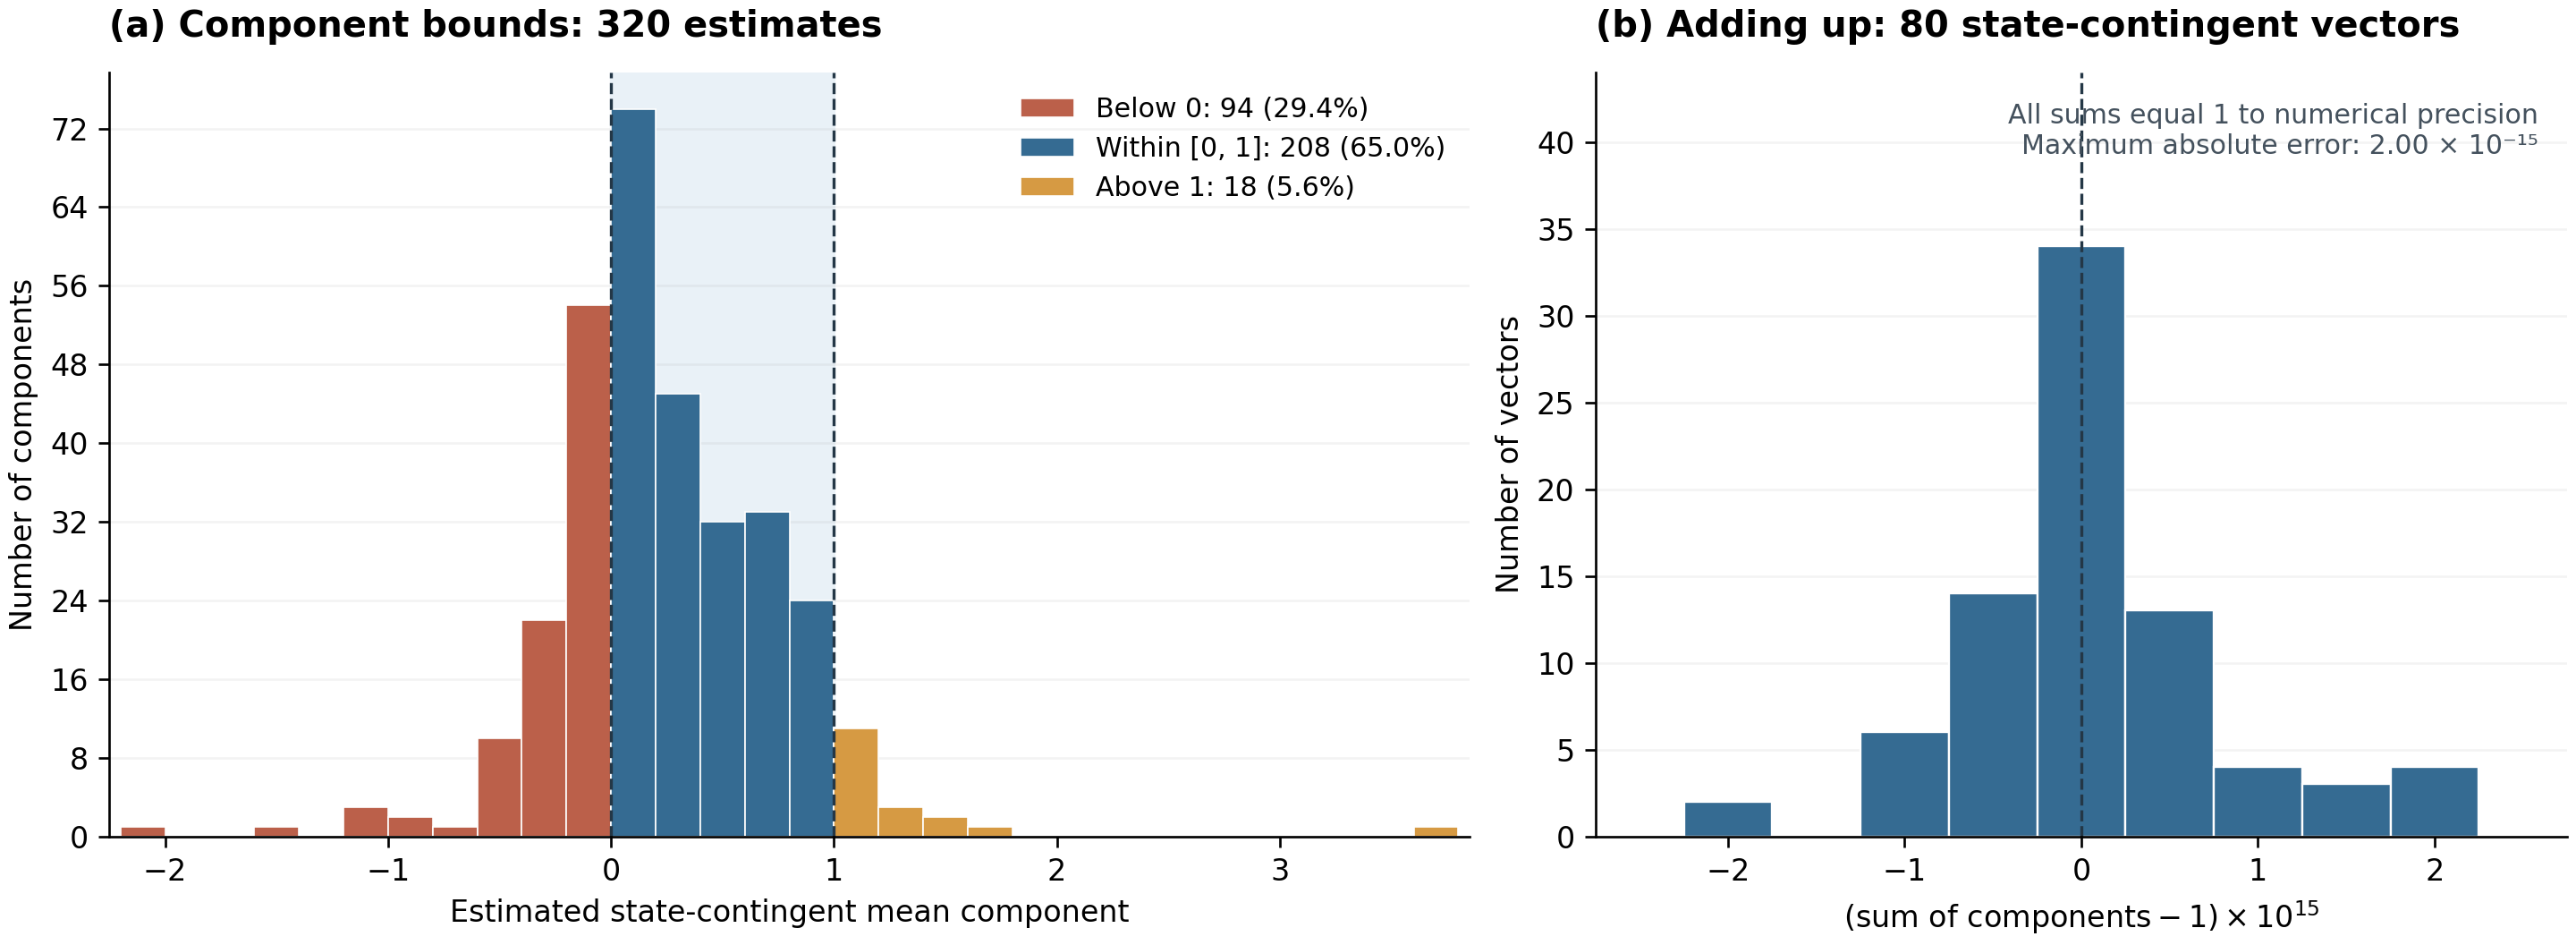
\includegraphics[width=1\linewidth]{State_contingent_Vec_dist.png}
    \caption{Distribution of Estimated State-contingent Means}
    \label{fig:state_mean_distribution}
\end{figure}

\begin{figure}[htbp]
    \centering
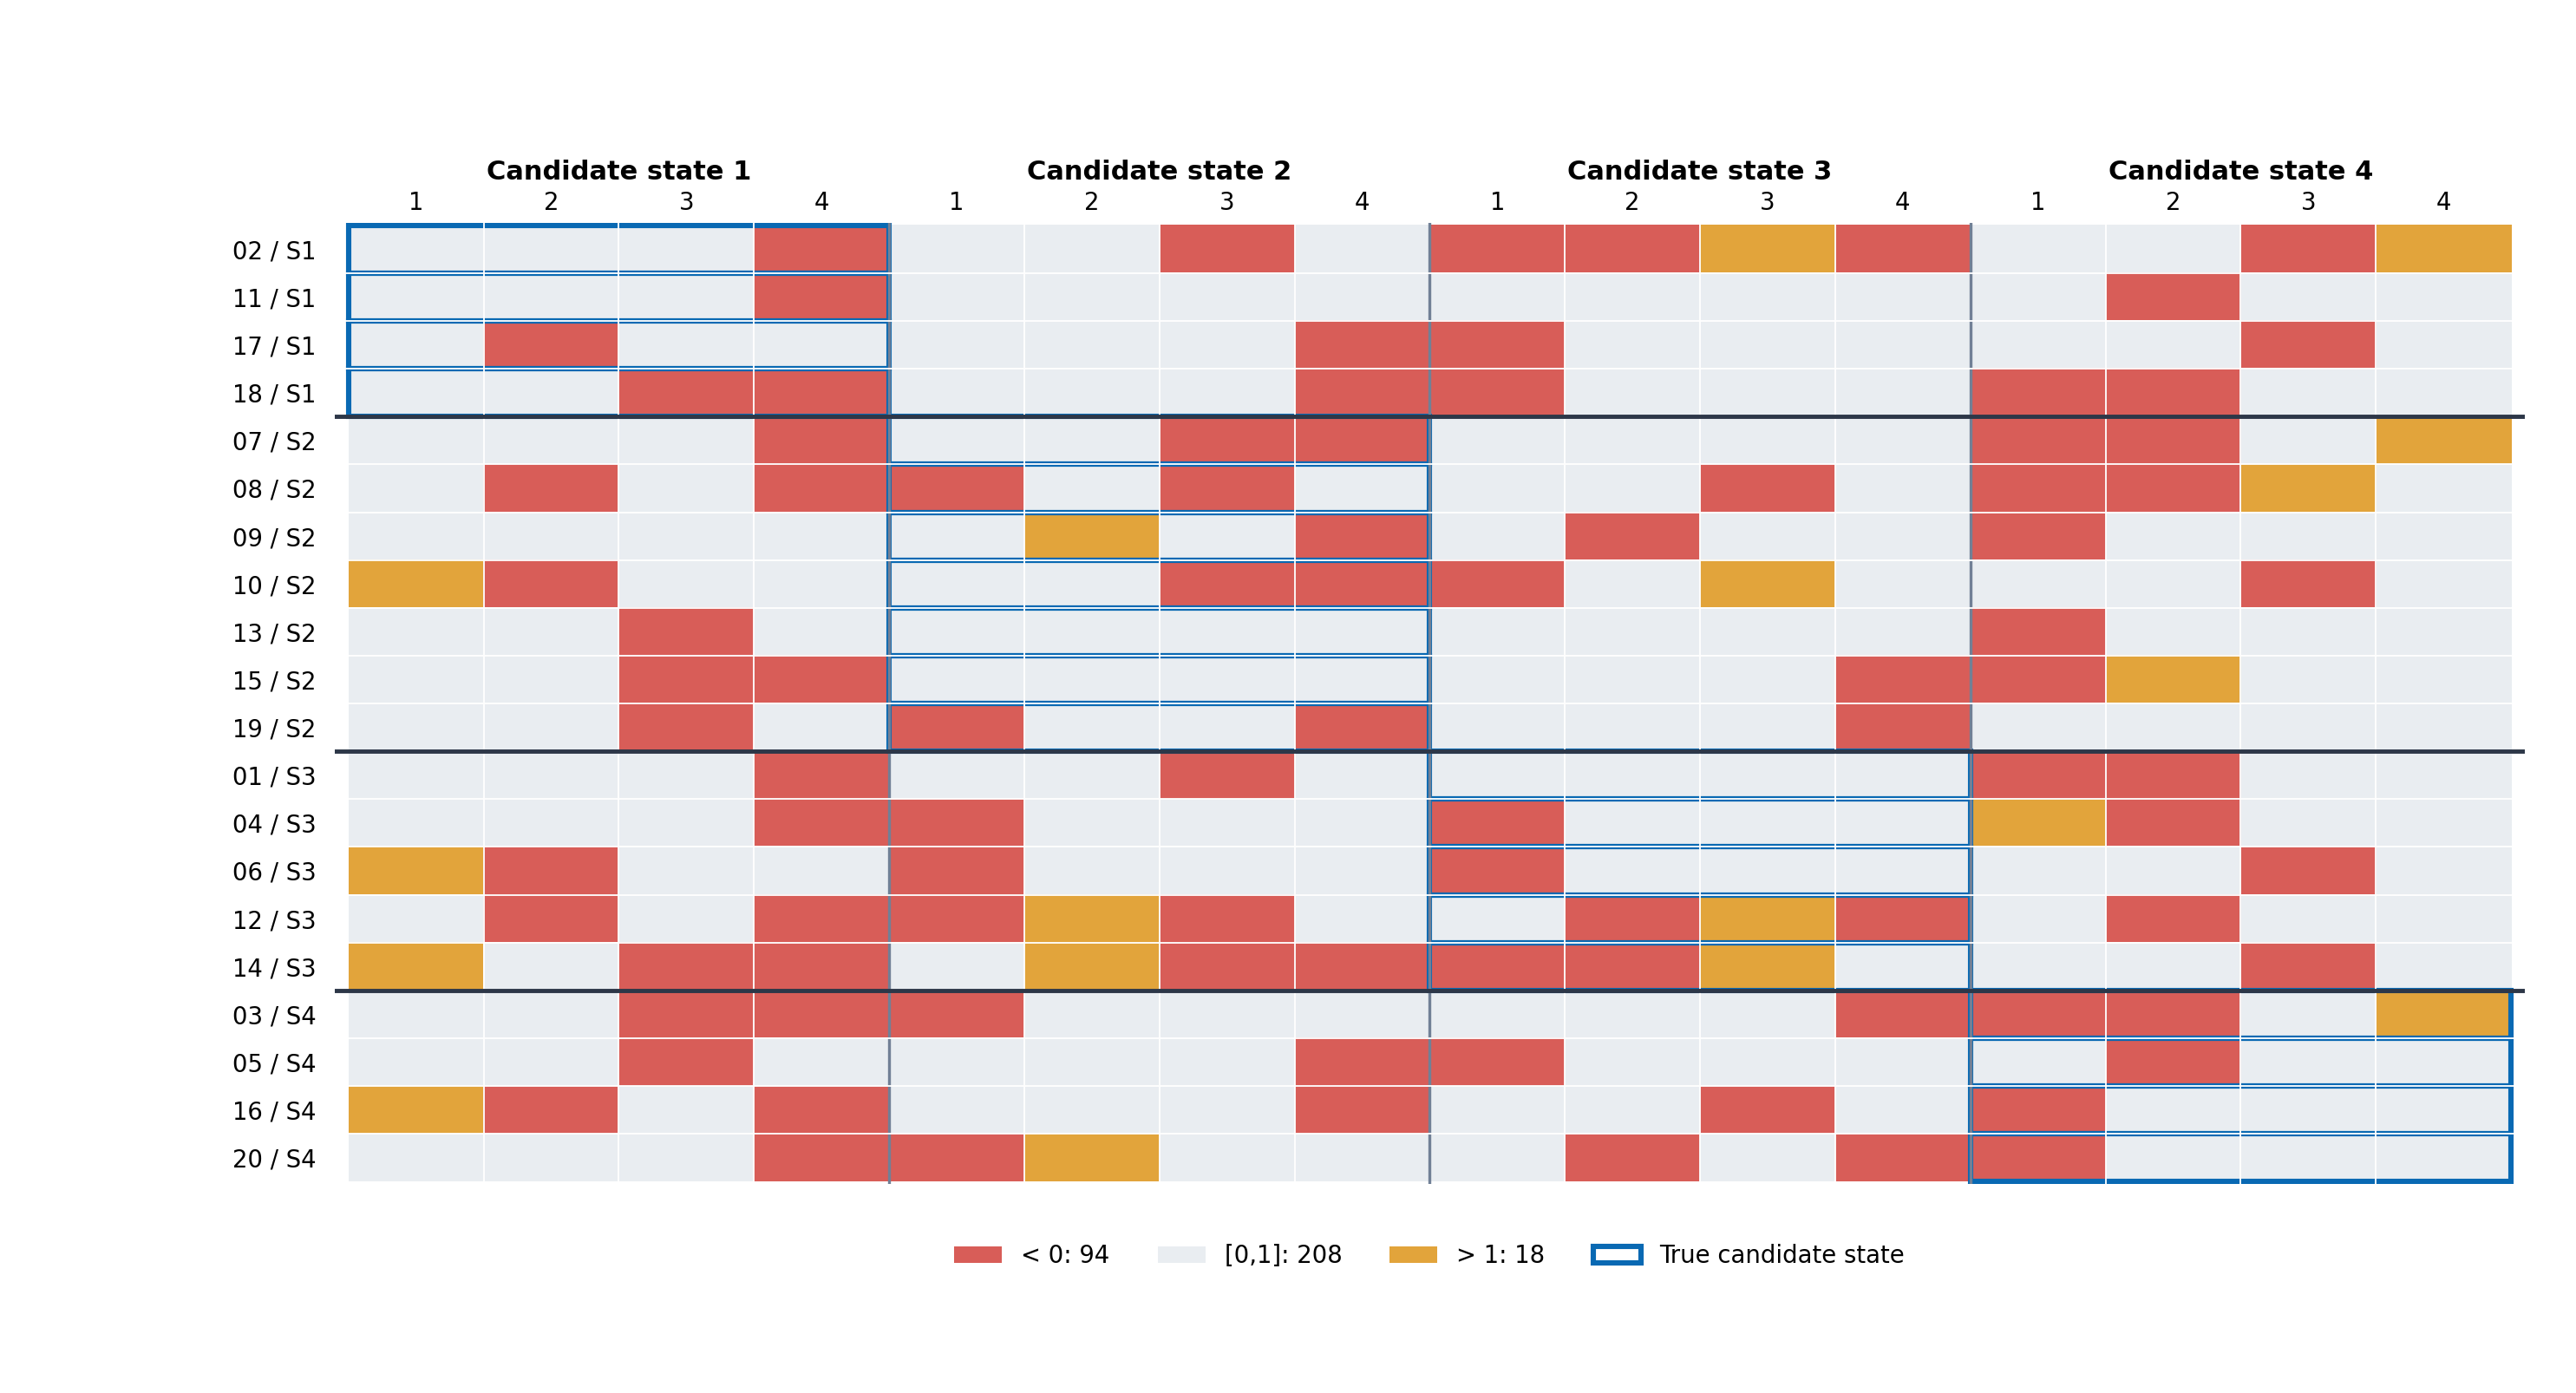
\includegraphics[width=0.99\textwidth,height=6.18in,keepaspectratio]{valid_grid.png}
\caption{Validity of Estimated State-contingent Means}
\label{validity}
\end{figure}

\begin{landscape}
\thispagestyle{plain}
\noindent
\begin{adjustbox}{max totalsize={\linewidth}{0.95\vsize},center}
\begin{minipage}{\linewidth}
\centering

\captionof{table}{NFT-Level Predictions and Accuracy across Alternative Matching Rules}
\label{alternative-matching}

\begingroup
\tiny
\renewcommand{\baselinestretch}{1}\selectfont
\setlength{\tabcolsep}{3pt}
\renewcommand{\arraystretch}{1.04}

\begin{tabular}{@{}cc*{11}{c}@{}}
\toprule
& &
\multicolumn{1}{c}{Four coordinates} &
\multicolumn{4}{c}{One coordinate} &
\multicolumn{3}{c}{Valid coordinates} &
\multicolumn{3}{c}{ Mean-belief rules and voting} \\
\cmidrule(lr){3-3}
\cmidrule(lr){4-7}
\cmidrule(lr){8-10}
\cmidrule(l){11-13}
NFT & True & Baseline OLS--IV
& $d=1$ & $d=2$ & $d=3$ & $d=4$
& Own $\geq1$ & Own $\geq2$ & Own $\geq3$
& Mean $\mu$ & Mean $\alpha$ & Vote \\
\midrule

2 & 1
& \textcolor{goodblue}{\bfseries 1}
& 4
& \textcolor{goodblue}{\bfseries 1}
& \textcolor{goodblue}{\bfseries 1}
& \textcolor{goodblue}{\bfseries 1}
& \textcolor{goodblue}{\bfseries 1}
& \textcolor{goodblue}{\bfseries 1}
& \textcolor{goodblue}{\bfseries 1}
& \textcolor{goodblue}{\bfseries 1}
& \textcolor{goodblue}{\bfseries 1}
& \textcolor{goodblue}{\bfseries 1} \\

11 & 1
& \textcolor{goodblue}{\bfseries 1}
& 2
& \textcolor{goodblue}{\bfseries 1}
& \textcolor{goodblue}{\bfseries 1}
& 2
& \textcolor{goodblue}{\bfseries 1}
& \textcolor{goodblue}{\bfseries 1}
& \textcolor{goodblue}{\bfseries 1}
& \textcolor{goodblue}{\bfseries 1}
& \textcolor{goodblue}{\bfseries 1}
& \textcolor{goodblue}{\bfseries 1} \\

17 & 1
& \textcolor{goodblue}{\bfseries 1}
& 4 & 3 & 2
& \textcolor{goodblue}{\bfseries 1}
& \textcolor{goodblue}{\bfseries 1}
& \textcolor{goodblue}{\bfseries 1}
& \textcolor{goodblue}{\bfseries 1}
& \textcolor{goodblue}{\bfseries 1}
& \textcolor{goodblue}{\bfseries 1}
& \textcolor{goodblue}{\bfseries 1} \\

18 & 1
& 2 & 4 & 3 & 4 & 3 & 2 & 2 & 2 & 3 & 3 & 3 \\

\addlinespace[2pt]

7 & 2
& 1 & \textcolor{goodblue}{\bfseries 2}
& 3 & 1 & 3 & 1 & 1 & 1 & 1 & 1 & 1 \\

8 & 2
& 3 & 3 & 1 & 1 & 3 & 4 & 1 & 3 & 1
& \textcolor{goodblue}{\bfseries 2}
& 1 \\

9 & 2
& 1 & 3 & 4
& \textcolor{goodblue}{\bfseries 2}
& 1
& \textcolor{goodblue}{\bfseries 2}
& \textcolor{goodblue}{\bfseries 2}
& 1 & 1 & 1 & 1 \\

10 & 2
& 4 & 4 & 3 & 1 & 1 & 1 & 1 & 4 & 1 & 1 & 1 \\

13 & 2
& \textcolor{goodblue}{\bfseries 2}
& \textcolor{goodblue}{\bfseries 2}
& 4 & 4 & 3 & \textcolor{goodblue}{\bfseries 2}
& \textcolor{goodblue}{\bfseries 2}
& \textcolor{goodblue}{\bfseries 2}
& 1 & 1 & 1 \\

15 & 2
& 1 & \textcolor{goodblue}{\bfseries 2}
& 1
& \textcolor{goodblue}{\bfseries 2}
& 1 & 1 & 1
& \textcolor{goodblue}{\bfseries 2}
& 1 & 1 & 1 \\

19 & 2
& 1 & 3 & 4 & 4 & 1 & 1 & 1 & 1 & 1 & 1 & 1 \\

\addlinespace[2pt]

1 & 3
& \textcolor{goodblue}{\bfseries 3}
& \textcolor{goodblue}{\bfseries 3}
& \textcolor{goodblue}{\bfseries 3}
& 1 & 2 & \textcolor{goodblue}{\bfseries 3}
& \textcolor{goodblue}{\bfseries 3}
& \textcolor{goodblue}{\bfseries 3}
& 1 & 1 & 1 \\

4 & 3
& 1 & 1 & 1 & 2
& \textcolor{goodblue}{\bfseries 3}
& 1 & 1 & 1 & 1 & 1 & 1 \\

6 & 3
& 4 & 4
& \textcolor{goodblue}{\bfseries 3}
& 2 & 2 & 1 & 1 & 4 & 1 & 1 & 1 \\

12 & 3
& 4 & 4 & 4 & 4 & 4 & \textcolor{goodblue}{\bfseries 3}
& 4 & 4 & 2
& \textcolor{goodblue}{\bfseries 3}
& 1 \\

14 & 3
& 1 & 2 & 1 & 1 & 2 & 1 & 4 & 4 & 1 & 1 & 1 \\

\addlinespace[2pt]

3 & 4
& 2 & 3 & 2
& \textcolor{goodblue}{\bfseries 4}
& 2 & \textcolor{goodblue}{\bfseries 4}
& 2 & 2 & 1 & 1 & 1 \\

5 & 4
& 1 & 2 & 3 & 2 & 1 & 1 & 1 & 1 & 1 & 1 & 1 \\

16 & 4
& 1 & 3 & 3 & 1 & 2 & 1
& \textcolor{goodblue}{\bfseries 4}
& \textcolor{goodblue}{\bfseries 4}
& 1 & 1 & 1 \\

20 & 4
& 1 & 3
& \textcolor{goodblue}{\bfseries 4}
& \textcolor{goodblue}{\bfseries 4}
& 2
& 2 & 2 & 1 & 1 & 1 & 1 \\

\midrule

State 1 & Correct
& 3/4 & 0/4 & 2/4 & 2/4 & 2/4 & 3/4 & 3/4 & 3/4 & 3/4 & 3/4 & 3/4 \\
& MAE
& 0.25 & 2.50 & 1.00 & 1.00 & 0.75 & 0.25 & 0.25 & 0.25 & 0.50 & 0.50 & 0.50 \\

\addlinespace[1pt]

State 2 & Correct
& 1/7 & 3/7 & 0/7 & 2/7 & 0/7 & 2/7 & 2/7 & 2/7 & 0/7 & 1/7 & 0/7 \\
& MAE
& 1.00 & 0.71 & 1.43 & 1.00 & 1.00 & 0.86 & 0.71 & 0.86 & 1.00 & 0.86 & 1.00 \\

\addlinespace[1pt]

State 3 & Correct
& 1/5 & 1/5 & 2/5 & 0/5 & 1/5 & 2/5 & 1/5 & 1/5 & 0/5 & 1/5 & 0/5 \\
& MAE
& 1.20 & 1.00 & 1.00 & 1.40 & 0.80 & 1.20 & 1.20 & 1.00 & 1.80 & 1.60 & 2.00 \\

\addlinespace[1pt]

State 4 & Correct
& 0/4 & 0/4 & 1/4 & 2/4 & 0/4 & 1/4 & 1/4 & 1/4 & 0/4 & 0/4 & 0/4 \\
& MAE
& 2.75 & 1.25 & 1.00 & 1.25 & 2.25 & 2.00 & 1.75 & 2.00 & 3.00 & 3.00 & 3.00 \\

\midrule

All NFTs & Correct
& 5/20 & 4/20 & 5/20 & 6/20 & 3/20 & 8/20 & 7/20 & 7/20 & 3/20 & 5/20 & 3/20 \\
& MAE
& 1.25 & 1.25 & 1.15 & 1.15 & 1.15 & 1.05 & 0.95 & 1.00 & 1.50 & 1.40 & 1.55 \\

\bottomrule
\end{tabular}
\par
\endgroup

\medskip
{\footnotesize
\renewcommand{\baselinestretch}{1}\selectfont
\raggedright
\textit{Notes:}
Blue color labels the correct predictions.
\textit{OLS--IV} matches the four estimated state-contingent means to mean
first-order beliefs by Euclidean distance.
A one-coordinate match uses coordinate $d$ alone, including
out-of-range estimates.
Own $\geq1$ is the candidate-specific valid-coordinate rule. For each candidate state, Own \(\geq1\) uses only coordinates whose estimates lie in \([0,1]\), and requires at least one such coordinate; Own $\geq2$ and $\geq3$
raise that minimum. Each candidate is scored by the root mean square of its
 valid-coordinate gaps.  Under Own $\geq 4$ some NFTs have no eligible candidate, so that column is omitted. Mean $\mu$ and Mean $\alpha$ choose the largest mean first-
and second-order belief; Vote uses plurality. These alternatives are exploratory.
\par}

\end{minipage}
\end{adjustbox}
\par
\end{landscape}

\clearpage
\subsection{Data and Code Availability}
The paper source files, the raw data used in the experiment, and the full open-source replication code for all reported empirical results are available at \url{https://github.com/malleshpai/robust-aggregation}. In particular, the repository includes the manuscript (\texttt{paper/}), raw data files (\texttt{Replication/data/raw/}), and the replication package with scripts, tests, and generated-table pipeline (\texttt{Replication/open/}).

\subsection{Consent and Ethical Approval}
The studies were all approved by the Department Ethics Review Committee (DERC) of NUS Department of Economics. For all studies, informed consent was obtained from the respondents using a consent form approved by DERC at the beginning of the online survey. Eligibility criteria required participants to be at least 18 years of age. Participants were informed of their rights to voluntary participation, confidentiality and anonymization of their responses, and minimal risks associated with participation.

\subsection{Detailed Survey Design}

\subsubsection{Knowledge Test}
Prior to eliciting participants' beliefs about NFT prices, we designed a brief knowledge assessment comprising six multiple-choice questions. The questions were selected according to two criteria: (1) they do not contain or imply any information about specific NFT prices or the price distribution in the NFT market, and (2) they only cover general concepts accessible to laypersons, avoiding any technical content that would require domain expertise. The full set of questions is provided below.

\textbf{Knowledge Assessment Questions:}

[1/6] What is ``minting'' an NFT?
\begin{enumerate}
    \item Save it to your phone
    \item \textit{Creating it and recording it on the blockchain}
    \item Uploading it to a gallery
    \item Selling it to the highest bidder
\end{enumerate}

[2/6] What is a common platform used for NFT trading and collecting?
\begin{enumerate}
    \item Google Photos
    \item Dropbox
    \item \textit{OpenSea}
    \item MetaMask
\end{enumerate}

[3/6] What are ``royalties'' in the NFT world?
\begin{enumerate}
    \item A reward for being an early buyer
    \item \textit{A way for artists to earn each time their NFT is resold}
    \item A fee paid to the blockchain network
    \item A code used to unlock NFTs
\end{enumerate}

[4/6] Which of the following best describes a ``utility NFT''?
\begin{enumerate}
    \item An NFT with no image or data
    \item An NFT used for mining cryptocurrency
    \item \textit{An NFT that provides additional functions, like access or benefits}
    \item An NFT that expires after 30 days
\end{enumerate}

[5/6] What is a ``PFP'' NFT often used for?
\begin{enumerate}
    \item \textit{Profile pictures and online identity}
    \item Online payments and banking
    \item Legal contracts
    \item Video streaming
\end{enumerate}

[6/6] Which of the following assets is fungible, unlike NFTs?
\begin{enumerate}
    \item A concert ticket
    \item A piece of digital art
    \item \textit{1 ETH (Ether)}
    \item A gaming skin with a unique serial number
\end{enumerate}

\subsubsection{Pedagogical Example}
Before participants begin evaluating NFTs, we present a brief pedagogical example to clarify the belief elicitation process. This is intended to mitigate potential ``learning'' effects. In the example, participants are guided through a simple scenario involving beliefs about ``\textit{Rain}'' versus ``\textit{No Rain}''. We then illustrate how the group average belief would be computed in the case where the population consists of two belief types. This example is intentionally designed to be unrelated to NFTs or price concepts, in order to avoid unintended priming effects or conceptual interference.

\begin{figure}[H]
\centering
\caption{Pedagogical Example on Self Belief}
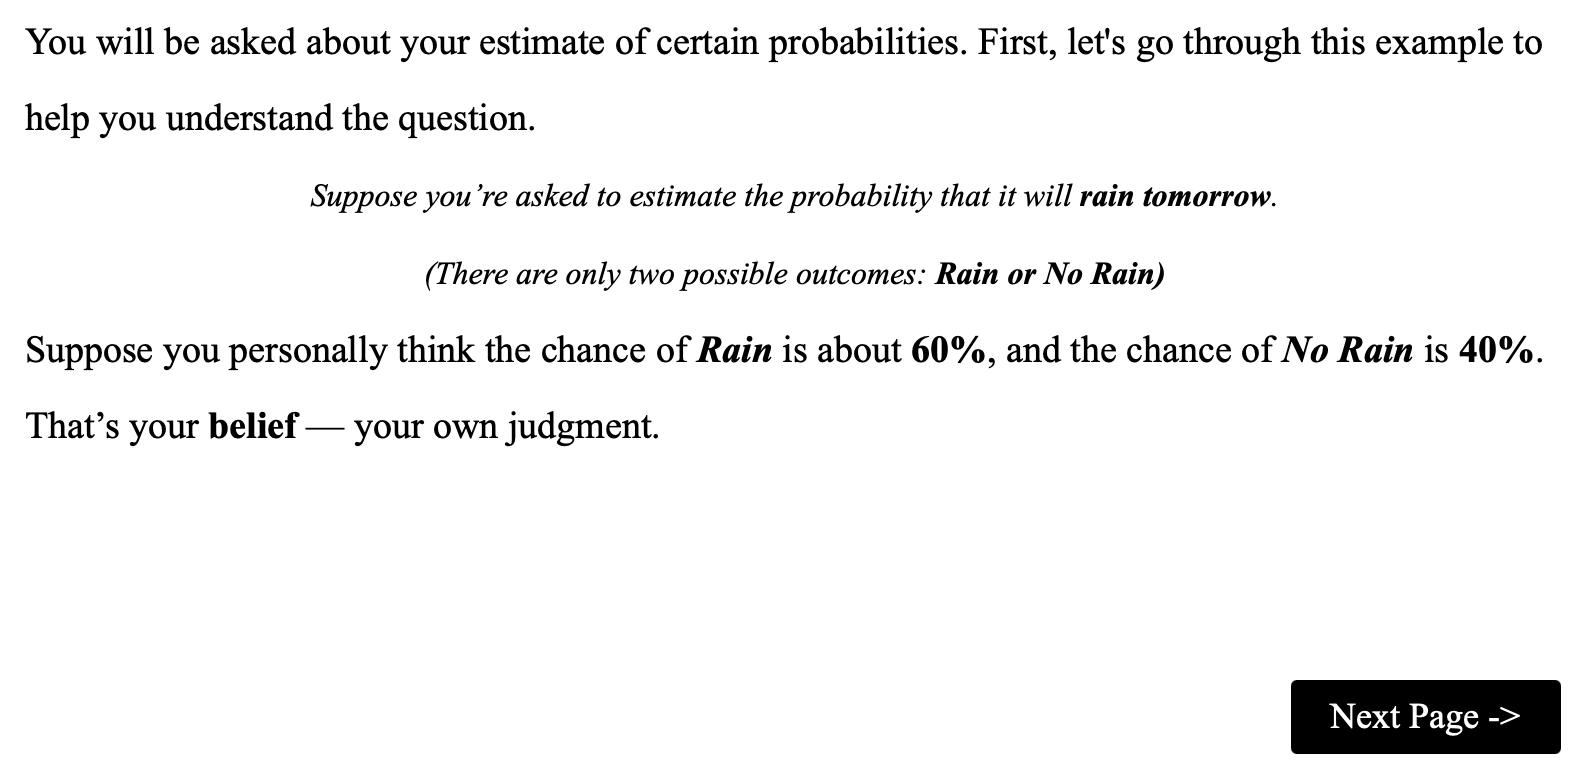
\includegraphics[width=0.9\linewidth]{images/peda1}
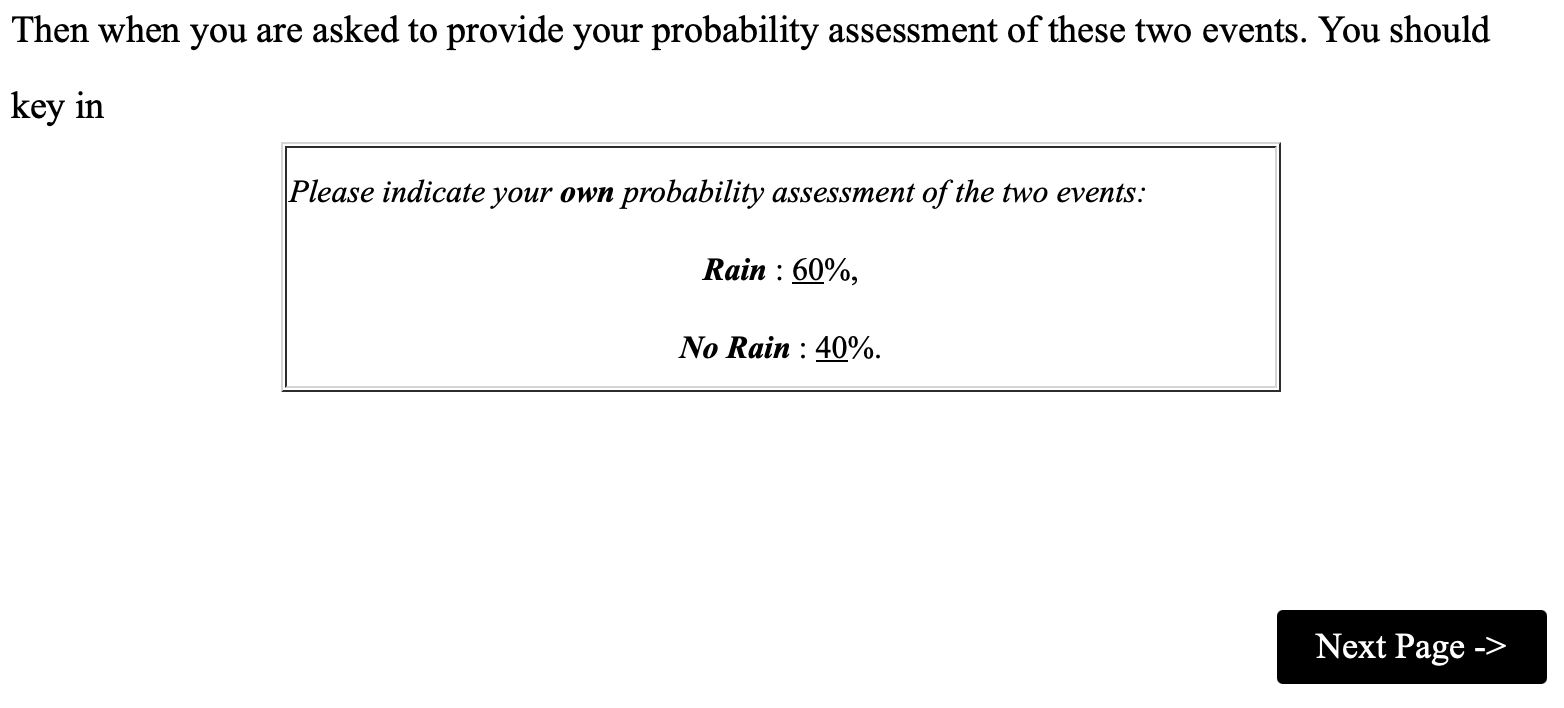
\includegraphics[width=0.9\linewidth]{images/peda2}
\end{figure}

\begin{figure}[H]
\centering
\caption{Pedagogical Example on Group Average Belief}

\vspace{0.5em}
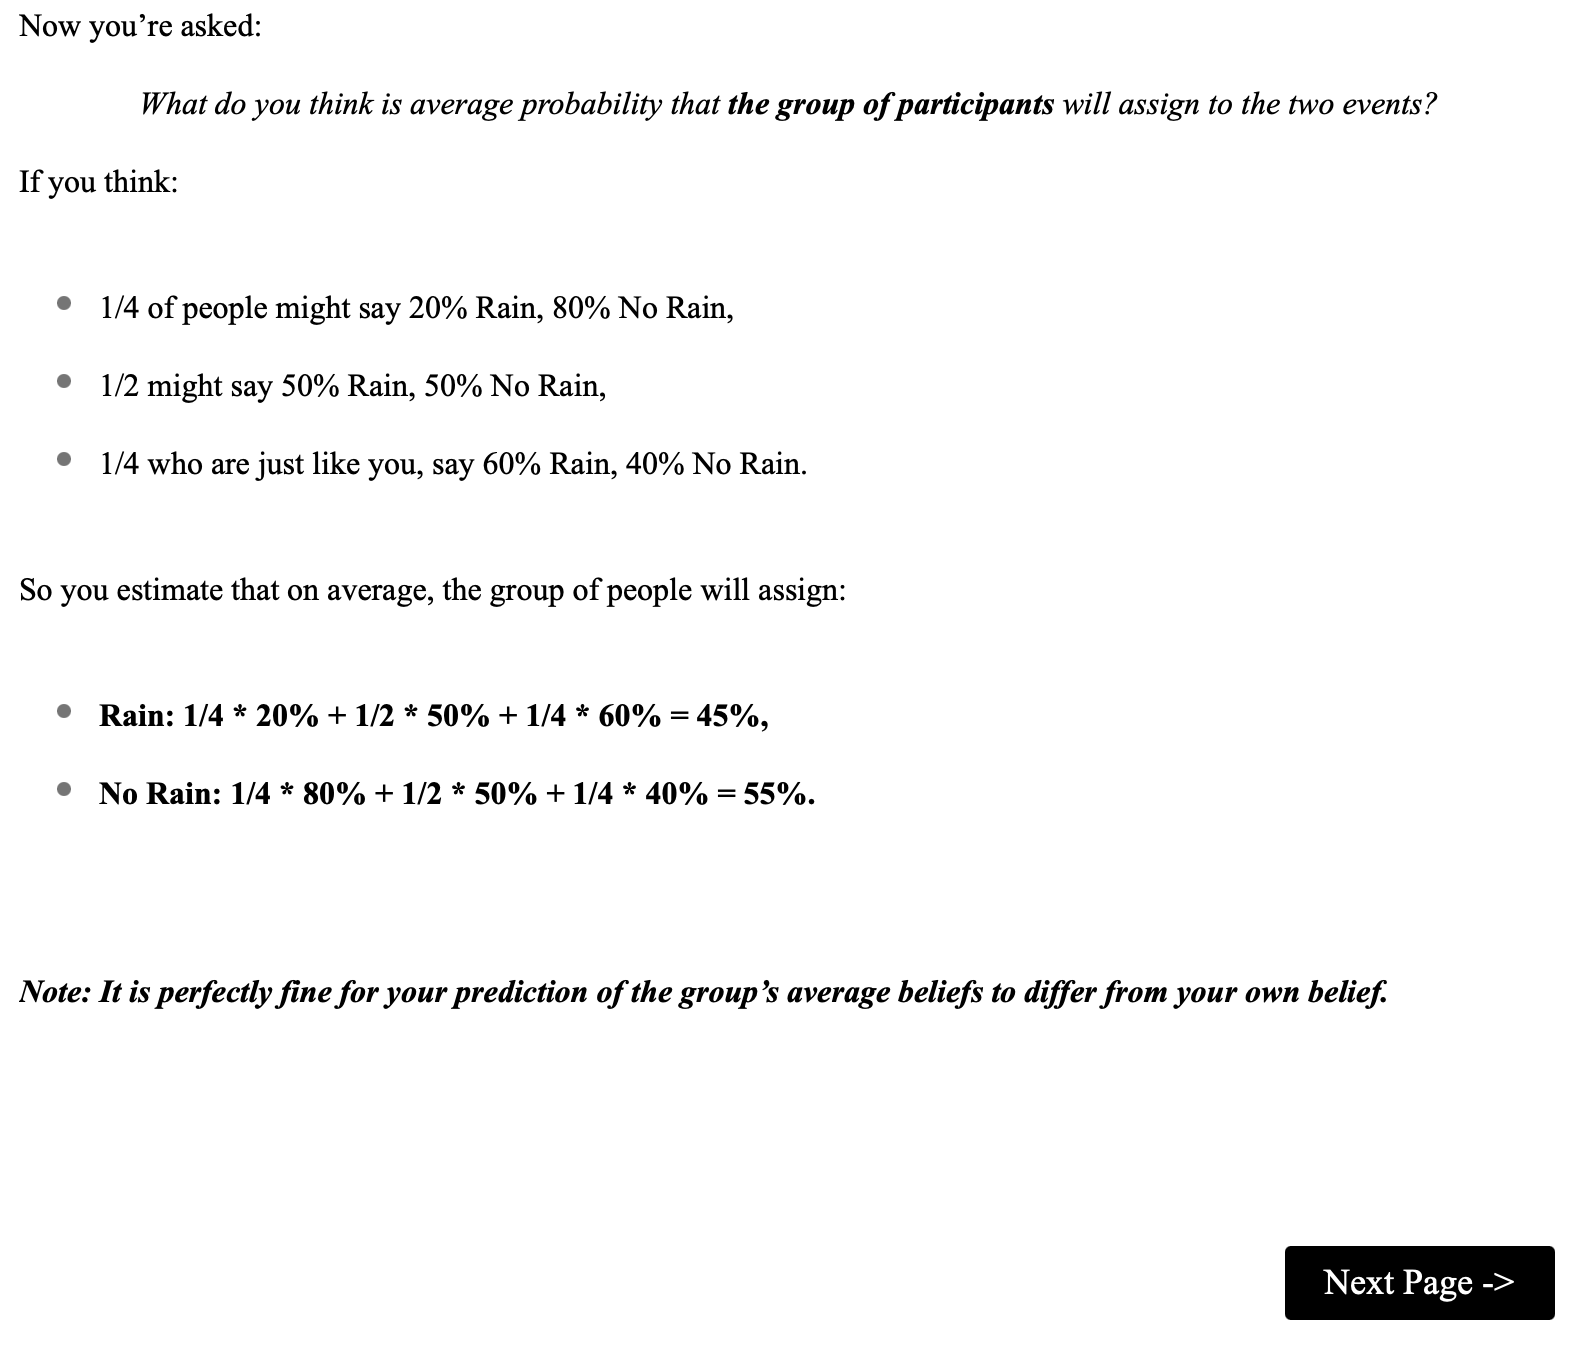
\includegraphics[width=0.9\linewidth]{images/peda3}
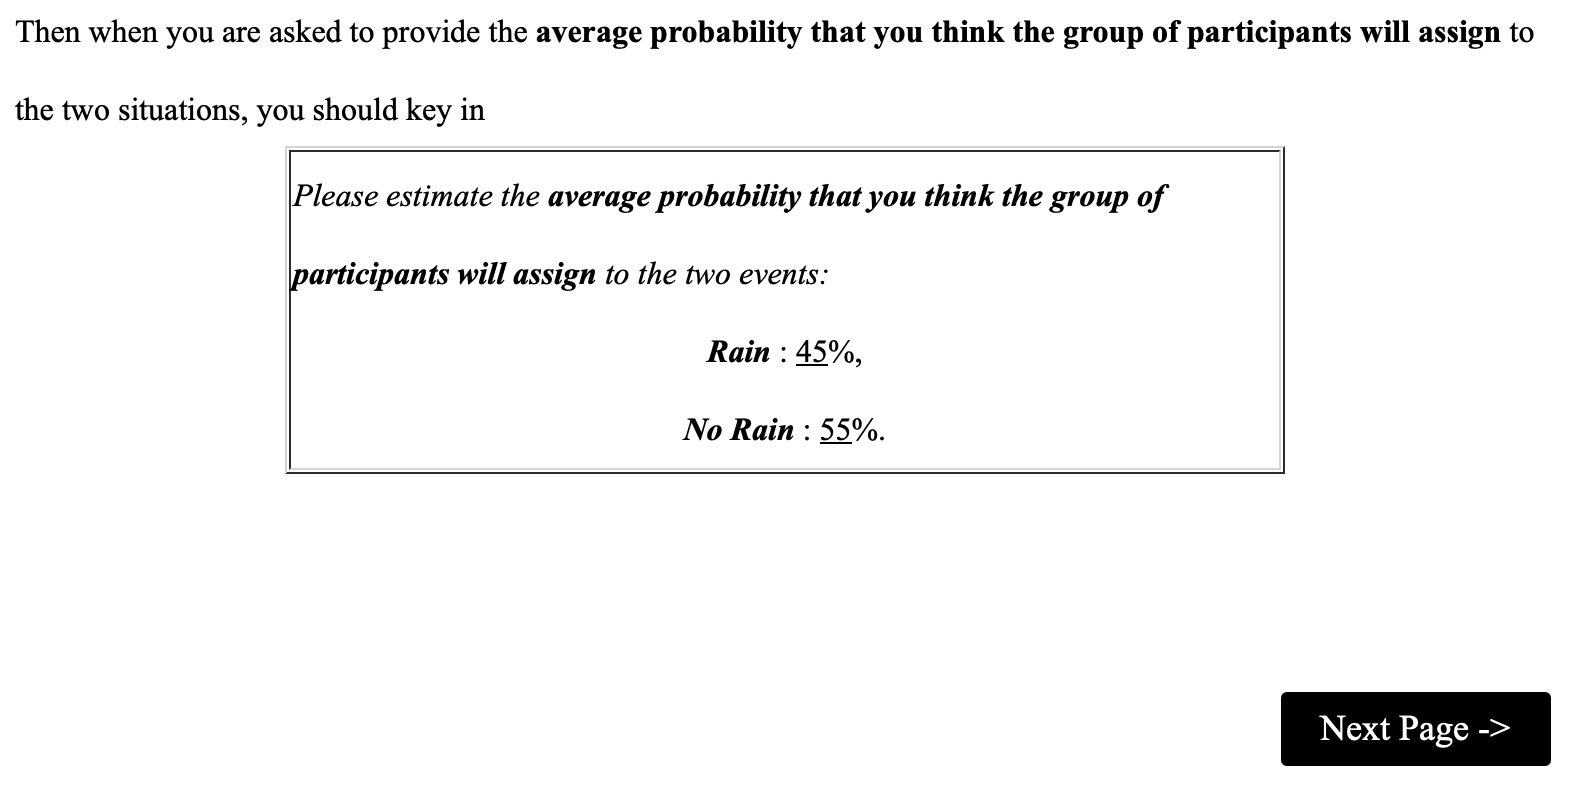
\includegraphics[width=0.9\linewidth]{images/peda4}
\end{figure}

\subsubsection{Belief Elicitation Interface}
In the main task, upon presentation of each NFT image, the belief elicitation interface first displays the self-belief question immediately below the image. Participants may freely enter numeric values into the four input fields corresponding to the predefined price ranges. The sum of these inputs is automatically computed and displayed in the ``Total'' row. When participants click the ``Next'' button to proceed to the subsequent question on group belief, the system verifies whether the inputs sum to exactly 100. If not, a warning message is triggered, and participants are required to revise their entries before continuing.

After participants successfully submit their self-belief responses, the NFT image remains on screen while the question below transitions to ask beliefs about the group average. To reduce the risk of inattention to this change, the group belief question is visually highlighted, and a brief explanation is provided to clarify that one's belief about the group may differ from one's own belief.

\begin{figure}[H]
\centering
\caption{Self Belief Elicitation Question}

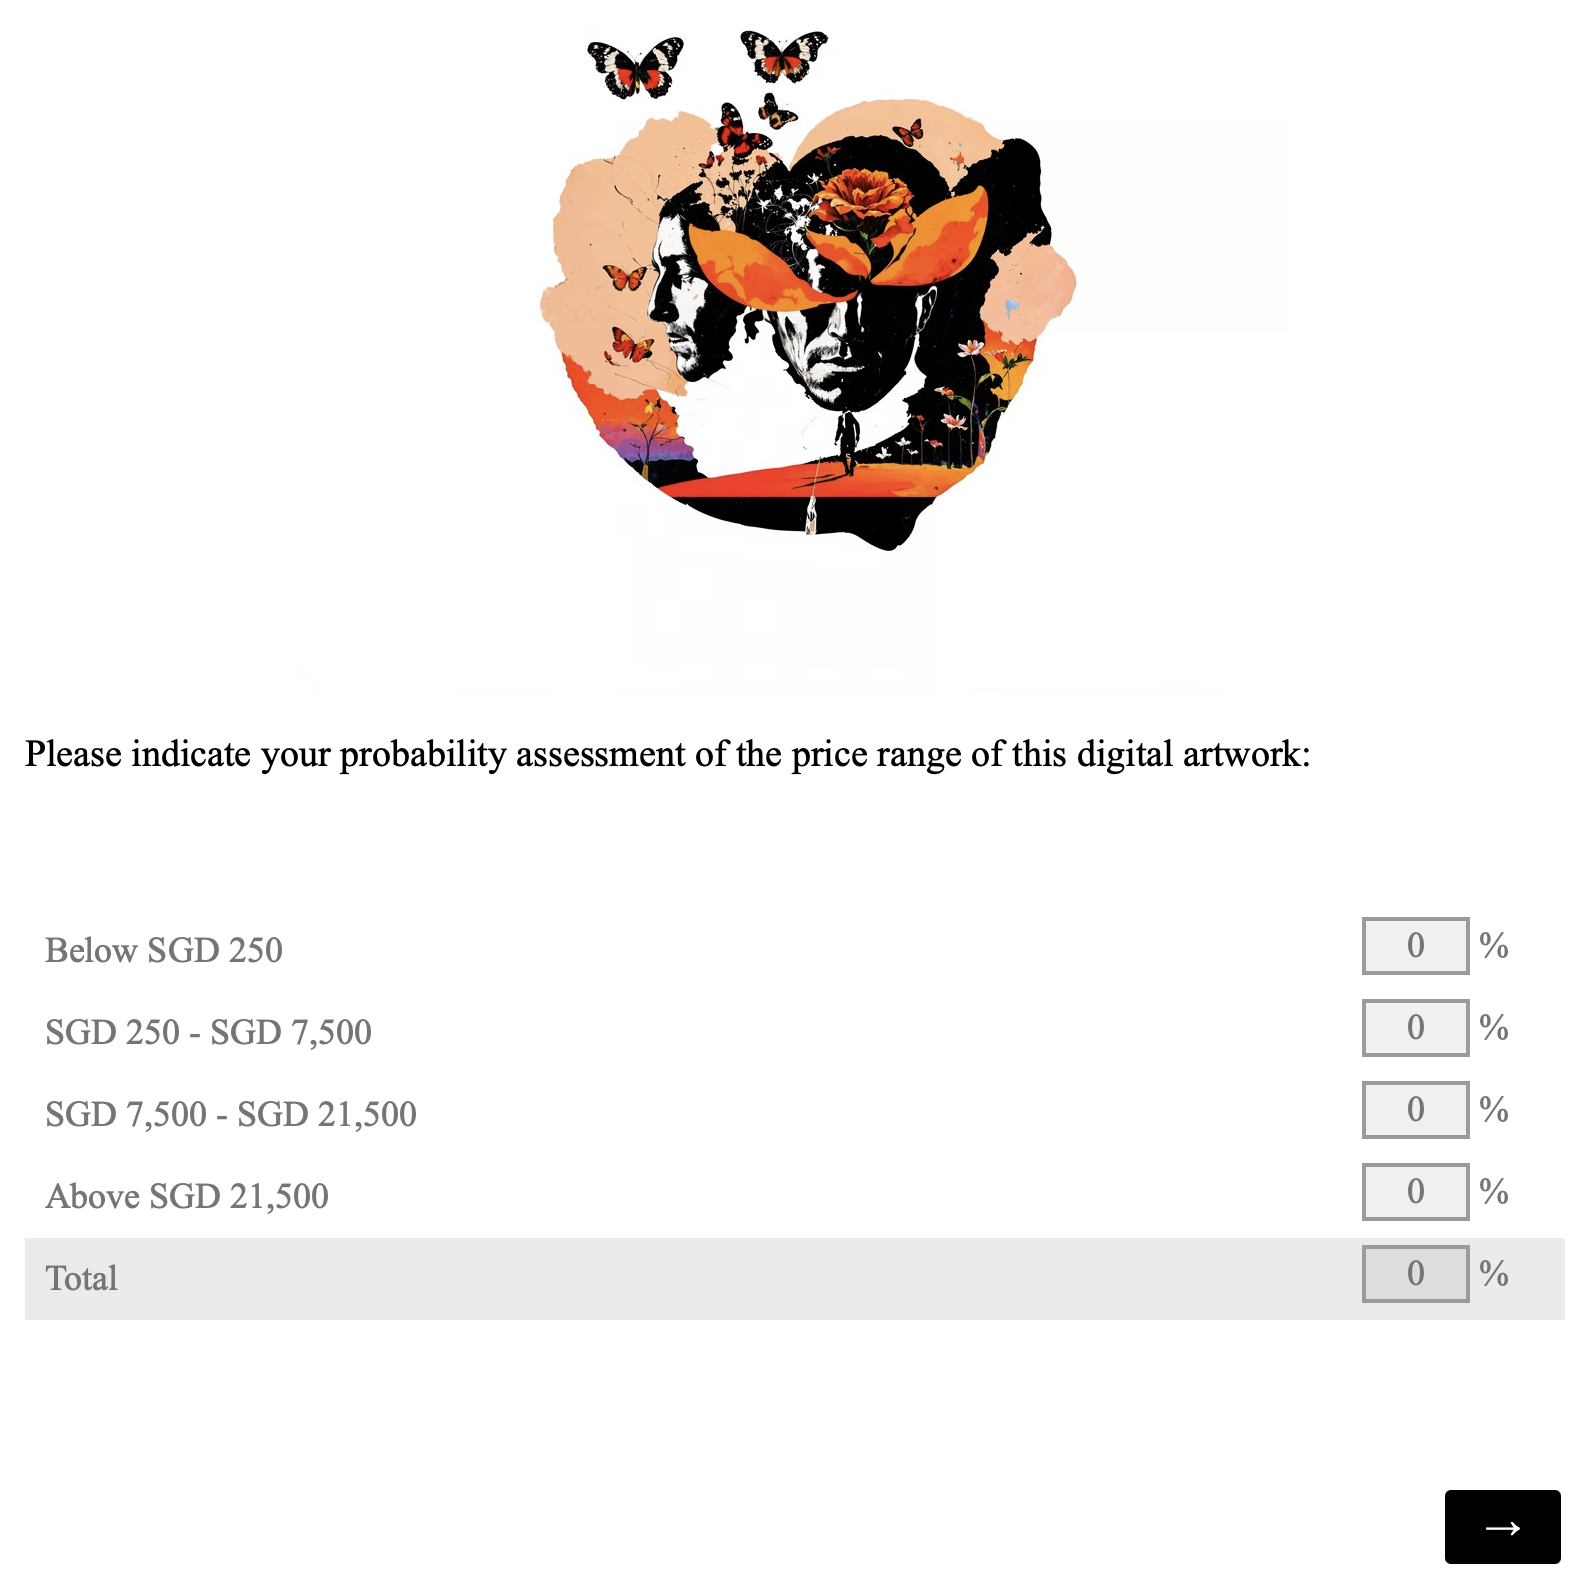
\includegraphics[width=0.9\linewidth]{images/FOB}
\end{figure}
\begin{figure}[H]
\centering
\caption{Group Belief Elicitation Question}

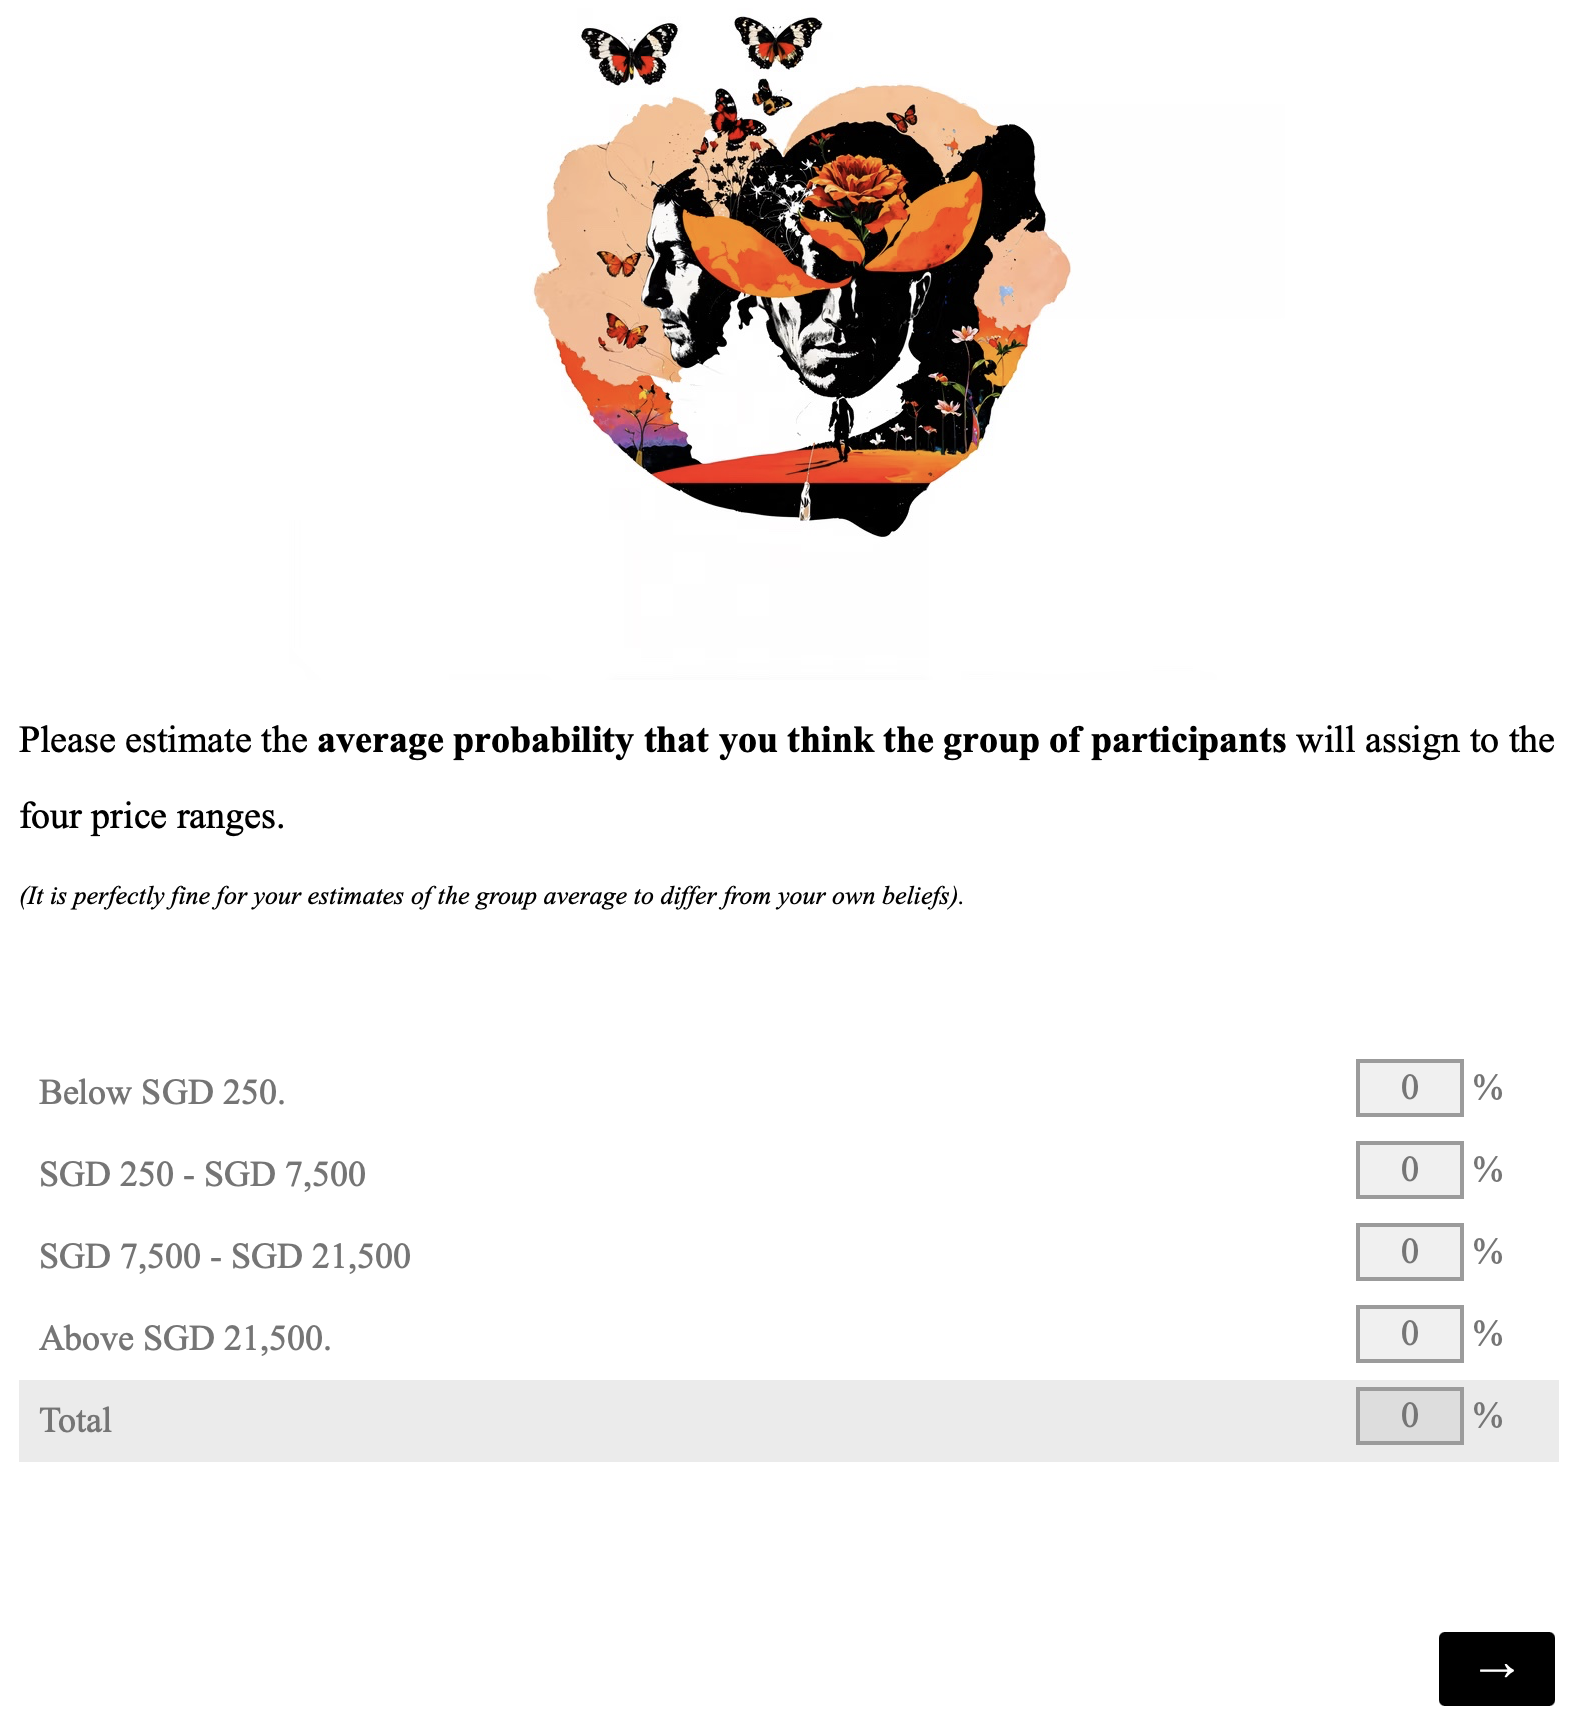
\includegraphics[width=0.9\linewidth]{images/SOB}
\end{figure}

\subsection{Robustness Checks}

 This subsection presents alternative specifications to verify the robustness of our main PMBA results. Table~\ref{tab:rob1} compares PMBA predictions across different implementation methods, including specifications with and without instrumental variables.

\subsubsection{Alternative Specifications}
Our baseline specification, reported in the main text, is estimated by OLS-IV with an intercept in both stages. As robustness checks, we vary (i) with/without intercept, (ii) unconstrained (OLS) vs.\ component-wise constrained (CLS), and (iii) IV vs.\ no-IV implementations. These exercises test whether the qualitative findings are sensitive to alternative structural assumptions.

The no-intercept specification with all four belief coordinates and the intercept specification with three coordinates are equivalent parameterizations in unconstrained OLS. Their identical predictions are therefore not an independent robustness result.

 To ensure structural interpretability of the coefficients as conditional probability beliefs,  we impose the restriction $\bar\mu_k^{(d)} \in [0,1]$. For the no-intercept version, this is written as
\[
\]
\[
\alpha_i^{(d)} = \sum_{k=1}^4 \bar\mu_k^{(d)} \tilde p_{ik} + \varepsilon_i^{(d)},
\quad \text{subject to} \quad \bar\mu_k^{(d)} \in [0,1].
\]

 Our implementation uses a logistic reparameterization rather than a general constrained least-squares solver. Specifically, we apply a logistic transformation,
\[
\qquad
\bar\mu_k^{(d)} = \frac{\exp(z_k^{(d)})}{1 + \exp(z_k^{(d)})},
\]
which maps unconstrained parameters  $z_k^{(d)} \in \mathbb{R}$ into the unit interval.\footnote{This reparameterization enforces component-wise bounds in $[0,1]$, but by itself it does not impose simplex summation.  In the with-intercept CLS column, the intercept and the three slopes are each constrained to lie in $[0,1]$. Since a nonbaseline mean is the intercept plus a slope, this column in effect requires every state mean to be at least the Range~4 mean, and allows means above one. In the no-intercept CLS column, we estimate four constrained coefficients directly as in the displayed equation above.}

\begin{table}[htbp]
\footnotesize
\centering
\tiny
\begin{threeparttable}
\caption{Robustness Check: PMBA Performance Across Different Implementation Methods}\label{tab:rob1}
\setlength{\tabcolsep}{4pt}\begin{tabular}{cccccccccc}
\toprule
\textbf{NFT} & \textbf{True State} & \multicolumn{2}{c}{Regression With Intercept} & \multicolumn{2}{c}{Regression Without Intercept} & \multicolumn{2}{c}{Regression Without IV} & Mean belief \\
\cmidrule(lr){3-4} \cmidrule(lr){5-6} \cmidrule(lr){7-8}
& & \textit{OLS} & \textit{CLS} & \textit{OLS} & \textit{CLS} & \textit{OLS} & \textit{CLS} & \\
\midrule
2  & 1 & 1 & 2 & 1 & 2 & 2 & 2 & 1 \\
11 & 1 & 1 & 1 & 1 & 1 & 1 & 4 & 1 \\
17 & 1 & 1 & 1 & 1 & 1 & 1 & 1 & 1 \\
18 & 1 & 2 & 2 & 2 & 2 & 3 & 4 & 3 \\
7  & 2 & 1 & 1 & 1 & 1 & 3 & 1 & 1 \\
8  & 2 & 3 & 2 & 3 & 2 & 3 & 1 & 1 \\
9  & 2 & 1 & 4 & 1 & 1 & 4 & 4 & 1 \\
10 & 2 & 4 & 4 & 4 & 4 & 2 & 2 & 1 \\
13 & 2 & 2 & 2 & 2 & 2 & 3 & 4 & 1 \\
15 & 2 & 1 & 1 & 1 & 1 & 1 & 1 & 1 \\
19 & 2 & 1 & 1 & 1 & 1 & 1 & 1 & 1 \\
1  & 3 & 3 & 4 & 3 & 3 & 2 & 4 & 1 \\
4  & 3 & 1 & 1 & 1 & 4 & 1 & 1 & 1 \\
6  & 3 & 4 & 4 & 4 & 4 & 2 & 2 & 1 \\
12 & 3 & 4 & 4 & 4 & 4 & 2 & 4 & 2 \\
14 & 3 & 1 & 1 & 1 & 1 & 1 & 1 & 1 \\
3  & 4 & 2 & 3 & 2 & 3 & 3 & 4 & 1 \\
5  & 4 & 1 & 1 & 1 & 1 & 1 & 1 & 1 \\
16 & 4 & 1 & 4 & 1 & 3 & 2 & 4 & 1 \\
20 & 4 & 1 & 4 & 1 & 1 & 2 & 2 & 1 \\
\midrule
\multicolumn{2}{r}{Average absolute error by range} & 0.25 & 0.50 & 0.25 & 0.50 & 0.75 & 1.75 & 0.50 \\
& & 1.00 & 1.00 & 1.00 & 0.86 & 1.00 & 1.14 & 1.00 \\
& & 1.20 & 1.40 & 1.20 & 1.00 & 1.40 & 1.40 & 1.80 \\
& & 2.75 & 1.00 & 2.75 & 2.00 & 2.00 & 1.25 & 3.00 \\
\midrule
Paired $t$-test & $p$-value:  & 0.0481 & 0.0331 & 0.0481 & 0.0176 & 0.0675 & 0.3123 & \\
\bottomrule
\end{tabular}

\begin{tablenotes}[flushleft]
\footnotesize
\item \textit{Notes:} The four rows under ``Average absolute error by range'' report the mean absolute error for each true price range (Ranges 1--4). The first four columns use IV-based implementations (with/without intercept, OLS/CLS); the next two columns report no-IV implementations. OLS-IV with intercept and OLS-IV without intercept produce identical state predictions in this sample.  The reported tests are one-sided item-level comparisons against the first-order mean-belief rule. They do not account for repeated respondents or establish instrument validity.
\end{tablenotes}
\end{threeparttable}
\end{table}

\subsubsection{First-stage fit}
Table~\ref{tab:firststage} reports, for each NFT, the number of participants, the number retained in the second stage, and the joint $F$ statistic of the six quiz indicators in the first-stage regression for each nonbaseline range. All 60 statistics are below 10.

\begin{table}[htbp]
\centering\small\caption{First-stage fit by NFT}\label{tab:firststage}
\begin{tabular}{rrrrrr}
\toprule
 & & & \multicolumn{3}{c}{First-stage $F$} \\
\cmidrule(lr){4-6}
NFT & $n$ & Retained & Range 1 & Range 2 & Range 3 \\
\midrule
1 & 102 & 102 & 1.77 & 2.67 & 1.55 \\
2 & 103 & 103 & 2.31 & 1.31 & 2.18 \\
3 & 101 & 101 & 0.68 & 1.81 & 1.16 \\
4 & 100 & 99 & 2.10 & 3.50 & 1.36 \\
5 & 101 & 101 & 0.87 & 1.45 & 0.29 \\
6 & 100 & 100 & 1.13 & 0.90 & 0.98 \\
7 & 97 & 97 & 1.25 & 1.36 & 0.81 \\
8 & 96 & 95 & 1.08 & 0.23 & 0.84 \\
9 & 93 & 93 & 1.74 & 1.09 & 1.62 \\
10 & 97 & 95 & 0.45 & 0.43 & 1.23 \\
11 & 99 & 98 & 3.96 & 0.89 & 1.93 \\
12 & 101 & 101 & 1.51 & 0.40 & 2.57 \\
13 & 102 & 102 & 1.23 & 1.14 & 0.89 \\
14 & 98 & 97 & 1.21 & 1.19 & 0.94 \\
15 & 100 & 100 & 3.52 & 1.09 & 2.95 \\
16 & 100 & 100 & 0.36 & 0.95 & 0.60 \\
17 & 94 & 94 & 0.84 & 1.39 & 0.66 \\
18 & 99 & 99 & 0.81 & 1.18 & 0.49 \\
19 & 104 & 104 & 0.50 & 0.72 & 0.54 \\
20 & 103 & 103 & 0.90 & 2.22 & 0.37 \\
\bottomrule
\end{tabular}
\begin{minipage}{.8\textwidth}\footnotesize
\emph{Notes:} Classical $F$ statistics for the joint significance of the six quiz indicators, with $(6,\,n-7)$ degrees of freedom. Retained participants have no negative fitted first-order probability.
\end{minipage}
\end{table}

\subsection{NFTs Used in the Experiment}

 This subsection provides the complete list of experimental materials. Table~\ref{tab:nft_list} displays all 20 NFTs used in the experiment, including their collection names, individual identifiers, actual market prices (in both ETH and SGD), and the price ranges they were assigned to for the belief elicitation task.

\begin{table}[htbp]
\centering
\caption{NFTs Used in the Experiment}\label{tab:nft_list}

\rotatebox{90}{%
\begin{minipage}{0.9\textheight} % swap width and height since rotated
\centering
\begin{tabular}{@{}rllrrr@{}}
\toprule
\textbf{ID} & \textbf{Collection} & \textbf{Number} & \textbf{Price (ETH)} & \textbf{Price (SGD)} & \textbf{Range} \\
\midrule
1 & Azuki & 2765 & 4 & 10102.96 & 3 \\
2 & BBKC & 5272 & 0.0003 & 0.76 & 1 \\
3 & Bored Ape & 4491 & 13 & 32834.62 & 4 \\
4 & Citizen & 3769 & 6 & 15154.44 & 3 \\
5 & CryptoPunk & 4297 & 39 & 98503.86 & 4 \\
6 & Doodle & 9355 & 3.4899 & 8814.58 & 3 \\
7 & Enchanter Arabella of the Villa & -- & 0.31 & 782.98 & 2 \\
8 & Human Unreadable & 73 & 1.65 & 4167.47 & 2 \\
9 & One Gravity & 1770 & 1.27 & 3207.69 & 2 \\
10 & Lil Pudgy & 20828 & 1.089 & 2750.53 & 2 \\
11 & Memory & 343 & 0.0758 & 191.45 & 1 \\
12 & Meridian & 942 & 3.5 & 8840.09 & 3 \\
13 & Mutant Ape & 7734 & 2.159 & 5453.07 & 2 \\
14 & Milady & 9026 & 4.49 & 11340.57 & 3 \\
15 & Predator, First Draft & 291 & 1.05 & 2652.03 & 2 \\
16 & Pudgy Penguin & 8693 & 9.88 & 24954.31 & 4 \\
17 & Supduck & 6639 & 0.017 & 42.94 & 1 \\
18 & The Forbidden Museum Hall & -- & 0.0455 & 114.92 & 1 \\
19 & Wealthy Hypio Babies & 5042 & 1.62 & 4091.70 & 2 \\
20 & GigaChad & 95 & 25 & 63143.50 & 4 \\
\bottomrule
\end{tabular}

\vspace{1em}
\noindent\textit{Note:} This table shows all 20 NFTs used in our experiment. Prices are listed in both ETH (Ethereum cryptocurrency) and SGD (Singapore Dollars). The \textbf{Range} column shows which of our four price categories each NFT falls into: 1 (SGD 0--250), 2 (SGD 250--7,500), 3 (SGD 7,500--21,500), or 4 (SGD 21,500+). We verified that all NFTs stayed in their assigned ranges during the experiment.
\end{minipage}
} % end rotatebox

\end{table}

\subsection{Replication of Surprisingly Popular Procedure}

 This subsection replicates the Surprisingly Popular (SP) procedure using our experimental data. Table~\ref{tab:sp_replication} shows the SP predictions for each NFT, comparing the average first-order beliefs with the average second-order beliefs to determine which states are ``surprisingly popular'' and providing statistical tests for the significance of these differences.

\begin{table}[htbp]\centering
\scriptsize
\begin{threeparttable}
\caption{Replication of Surprisingly Popular (SP) Procedure Results}\label{tab:sp_replication}
\sisetup{table-format=2.2, table-number-alignment=center}
\setlength{\tabcolsep}{4pt}
\renewcommand{\arraystretch}{0.95}
\begin{tabular}{ccccc}
\toprule
\textbf{NFT} & \textbf{True State (Range)} & $\hat{\mu}_{(1\&2)}$ & \textbf{Mean of }$\alpha_{(1\&2)}$ & \textbf{SP Prediction}\\
\midrule
2 & 1\&2 (1) & 68.73\% & 69.93\% & 3\&4 \\
   \textit{(N=103)} & & & (0.3139) & \\

11 & 1\&2 (1) & 63.32\% & 62.52\% & 1\&2 \\
    \textit{(N=99)} & & & (0.3973) & \\

17 & 1\&2 (1) & 80.10\% & 77.34\% & 1\&2 \\
   \textit{(N=94)} & & & (0.1251) & \\

18 & 1\&2 (1) & 48.74\% & 45.84\% & 1\&2 \\
   \textit{(N=99)} & & & (0.1577) & \\
\midrule
7 & 1\&2 (2) & 77.27\% & 78.16\% & 3\&4 \\
  \textit{(N=97)} & & & (0.3506) & \\

8 & 1\&2 (2) & 65.39\% & 66.99\% & 3\&4 \\
   \textit{(N=96)} & & & (0.2805) & \\

9 & 1\&2 (2) & 65.03\% & 60.72\% & 1\&2 \\
   \textit{(N=93)} & & & (0.0864) & \\

10 & 1\&2 (2) & 75.25\% & 75.73\% & 3\&4 \\
    \textit{(N=97)} & & & (0.4268) & \\

13 & 1\&2 (2) & 59.95\% & 61.73\% & 3\&4 \\
    \textit{(N=102)} & & & (0.2943) & \\

15 & 1\&2 (2) & 75.48\% & 70.10\% & 1\&2 \\
    \textit{(N=100)} & & & (0.0254) & \\

19 & 1\&2 (2) & 77.39\% & 73.41\% & 1\&2 \\
    \textit{(N=104)} & & & (0.0713) & \\
\midrule
1 & 3\&4 (3) & 65.93\% & 64.62\% & 1\&2 \\
   \textit{(N=102)} & & & (0.3261) & \\

4 & 3\&4 (3) & 73.74\% & 75.15\% & 3\&4 \\
   \textit{(N=100)} & & & (0.2875) & \\

6 & 3\&4 (3) & 72.64\% & 72.36\% & 1\&2 \\
   \textit{(N=100)} & & & (0.4562) & \\

12 & 3\&4 (3) & 56.52\% & 51.82\% & 1\&2 \\
    \textit{(N=101)} & & & (0.0586) & \\

14 & 3\&4 (3) & 80.86\% & 80.41\% & 1\&2 \\
   \textit{(N=98)} & & & (0.4291) & \\
\midrule
3 & 3\&4 (4) & 54.24\% & 57.20\% & 3\&4 \\
  \textit{(N=101)} & & & (0.1874) & \\

5 & 3\&4 (4) & 77.07\% & 77.17\% & 3\&4 \\
  \textit{(N=101)} & & & (0.4839) & \\

16 & 3\&4 (4) & 72.01\% & 74.99\% & 3\&4 \\
   \textit{(N=100)} & & & (0.1236) & \\

20 & 3\&4 (4) & 64.76\% & 62.74\% & 1\&2 \\
    \textit{(N=103)} & & & (0.2470) & \\

\bottomrule
\end{tabular}

\begin{tablenotes}[flushleft]\footnotesize
\item \textit{Notes:} This table shows the belief-based binary SP comparison. We group the four price ranges into two: ``low prices'' (Ranges 1 \& 2) and ``high prices'' (Ranges 3 \& 4). For each NFT, the number in parentheses is the one-sided $p$-value for testing whether $\hat{\mu}_{(1\&2)}-\text{Mean}(\alpha_{(1\&2)})=0$. These tests compare reported means within each item. They are not tests of classification accuracy.
\end{tablenotes}
\end{threeparttable}
\end{table}

\end{document}
